\documentclass[a4paper,11pt]{ltjsarticle}
\usepackage[top=18mm,bottom=18mm,left=20mm,right=20mm]{geometry}
\usepackage{luatexja-fontspec}
\setmainjfont{Noto Serif CJK JP}[BoldFont=Noto Sans CJK JP Bold]
\setsansjfont{Noto Sans CJK JP}[BoldFont=Noto Sans CJK JP Bold]
\usepackage{amsmath,amssymb}
\usepackage{enumitem}
\usepackage{fancyhdr}
\usepackage{needspace}
\usepackage{multicol}
\usepackage[most]{tcolorbox}

\newtcolorbox{kai}{enhanced,breakable,colback=white,colframe=black,boxrule=0pt,
  borderline west={0.8pt}{0pt}{black},arc=0pt,left=8pt,right=0pt,top=2pt,bottom=2pt,
  before skip=3pt,after skip=8pt}

\pagestyle{fancy}
\fancyhf{}
\fancyhead[L]{\small\sffamily 数学Ⅱ・B・C 類題集}
\fancyhead[R]{\small\sffamily\leftmark}
\fancyfoot[C]{\small\thepage}
\renewcommand{\headrulewidth}{0.4pt}
\setlength{\parindent}{0pt}
\setlength{\parskip}{0.25em}
\setlist[enumerate,1]{label={(\arabic*)},leftmargin=2.2em,itemsep=2pt,topsep=2pt}

% 問題
\newcommand{\mon}[2]{\Needspace{7\baselineskip}\vspace{10pt}%
  {\sffamily\bfseries 類題 #1\quad #2\par}\vspace{2pt}\hrule\vspace{4pt}}
% 解答
\newcommand{\ans}[2]{\Needspace{5\baselineskip}\vspace{6pt}%
  {\sffamily\bfseries 類題 #1\quad #2}\par}
\newcommand{\point}[1]{\textsf{\bfseries ▶ #1}}
\newcommand{\rpt}[1]{0.\dot{#1}}

\usepackage{tikz}
\usetikzlibrary{calc,intersections}
\newcommand{\ax}[4]{\draw[->] (#1,0)--(#2,0) node[right]{\scriptsize $x$};
  \draw[->] (0,#3)--(0,#4) node[above]{\scriptsize $y$};
  \node[below left] at (0,0){\scriptsize O};}
\newcommand{\shou}[2]{\clearpage\markboth{#1\quad #2}{}%
  {\sffamily\bfseries\LARGE #1\quad #2\par}\vspace{2pt}\hrule height 1.2pt\vspace{4pt}}
\newcommand{\shouans}[2]{\Needspace{8\baselineskip}\vspace{10pt}\markboth{解答\quad #1\quad #2}{}%
  {\sffamily\bfseries\Large #1\quad #2\par}\vspace{2pt}\hrule height 0.8pt\vspace{2pt}}

\begin{document}
\thispagestyle{empty}
\begin{center}
\vspace*{50mm}
{\sffamily\bfseries\Huge 数学Ⅱ・B・C 類題集\par}
\vspace{8mm}
{\sffamily\Large 基礎問 類題1〜183\par}
\vspace{15mm}
\begin{minipage}{0.75\linewidth}\small
類題の番号は基礎問の番号に対応している．基礎問を学習したあと，同じテーマの問題が解けるかを確かめるのに使う．解答は後半にまとめてある．
\end{minipage}
\end{center}
\clearpage
\setcounter{page}{1}
\shou{第1章}{式と証明}
\mon{1}{3次式の展開}
次の式を展開せよ．
\[\text{(1)}\ (2x-y)^3\qquad\text{(2)}\ (a+2)(a^2-2a+4)\qquad\text{(3)}\ (x-1)(x^2+x+1)(x^3+1)\]

\mon{2}{3次式の因数分解}
次の式を因数分解せよ．
\[\text{(1)}\ 27x^3-8\qquad\text{(2)}\ x^3+6x^2y+12xy^2+8y^3\qquad\text{(3)}\ x^6-64\]

\mon{3}{パスカルの三角形}
パスカルの三角形を5段目までかき，それを利用して $(a+b)^5$ を展開せよ．

\mon{4}{2項定理・多項定理}
\begin{enumerate}
\item $(2x-1)^6$ の展開式における $x^4$ の係数を求めよ．
\item $\left(x^2-\dfrac2x\right)^6$ の展開式における定数項を求めよ．
\item $(x+y+2z)^5$ の展開式における $x^2yz^2$ の係数を求めよ．
\end{enumerate}

\mon{5}{整式のわり算}
\begin{enumerate}
\item $2x^3-3x^2+4x-5$ を $x^2-x+2$ でわったときの商と余りを求めよ．
\item 整式 $A$ を $x+2$ でわると，商が $x^2-3$，余りが $5$ であった．$A$ を求めよ．
\end{enumerate}

\mon{6}{分数式の計算}
次の式を計算せよ．
\[\text{(1)}\ \ \frac1{x-1}-\frac1{x+1}-\frac2{x^2+1}\qquad\qquad\text{(2)}\ \ \frac{x^2-x-6}{x^2-4}\times\frac{x^2+3x+2}{x^2-9}\]

\mon{7}{繁分数式の計算}
次の式を簡単にせよ．
\[\text{(1)}\ \ \frac{1}{1-\dfrac{1}{1-\dfrac1x}}\qquad\qquad\text{(2)}\ \ \frac{\dfrac1x-\dfrac1y}{\dfrac1{x^2}-\dfrac1{y^2}}\]

\mon{8}{式の値}
$x+\dfrac1x=4$ のとき，次の式の値を求めよ．
\[\text{(1)}\ x^2+\frac1{x^2}\qquad\text{(2)}\ x^3+\frac1{x^3}\qquad\text{(3)}\ \left(x-\frac1x\right)^2\]

\mon{9}{比例式（Ⅰ）}
$\dfrac x2=\dfrac y3=\dfrac z4\ (\neq0)$ のとき，次の式の値を求めよ．
\[\text{(1)}\ \ \frac{x+y+z}{x-y+z}\qquad\qquad\text{(2)}\ \ \frac{xy+yz+zx}{x^2+y^2+z^2}\]

\mon{10}{比例式（Ⅱ）}
$\dfrac{b+c}{a}=\dfrac{c+a}{b}=\dfrac{a+b}{c}=k$ のとき，$k$ の値を求めよ．

\mon{11}{恒等式}
\begin{enumerate}
\item 等式 $a(x+1)^2+b(x+1)+c=2x^2-x+3$ が $x$ についての恒等式となるように，定数 $a,\ b,\ c$ の値を定めよ．
\item 等式 $\dfrac{1}{(x+1)(x+3)}=\dfrac{a}{x+1}+\dfrac{b}{x+3}$ が恒等式となるように，定数 $a,\ b$ の値を定めよ．
\end{enumerate}

\mon{12}{等式の証明}
\begin{enumerate}
\item $a+b+c=0$ のとき，$a^3+b^3+c^3=3abc$ であることを示せ．
\item $\dfrac ab=\dfrac cd$ のとき，$\dfrac{a+c}{b+d}=\dfrac{a-2c}{b-2d}$ であることを示せ．ただし，分母は0でないとする．
\end{enumerate}

\mon{13}{不等式の証明}
\begin{enumerate}
\item 実数 $x,\ y$ について，$x^2+y^2\geqq2(x+y)-2$ を示せ．また，等号が成りたつのはどのようなときか．
\item $x>0$ のとき，$x+\dfrac9x\geqq6$ を示せ．また，等号が成りたつ $x$ の値を求めよ．
\item $a>0$，$b>0$ のとき，$\sqrt a+\sqrt b>\sqrt{a+b}$ を示せ．
\end{enumerate}

\shou{第2章}{複素数と方程式}
\mon{14}{2次方程式の解}
次の2次方程式を複素数の範囲で解け．
\[\text{(1)}\ \ x^2+4=0\qquad\qquad\text{(2)}\ \ 3x^2-2x+1=0\]

\mon{15}{複素数の計算（Ⅰ）}
次の式を計算し，$a+bi$（$a,\ b$ は実数）の形で表せ．
\[\text{(1)}\ (2+3i)(1-2i)\qquad\text{(2)}\ (3-i)^2\qquad\text{(3)}\ \frac{1+i}{1-i}\]

\mon{16}{複素数の計算（Ⅱ）}
\begin{enumerate}
\item $(1+i)^8$ を計算せよ．
\item $(x+yi)(2-i)=5+5i$ をみたす実数 $x,\ y$ を求めよ．
\end{enumerate}

\mon{17}{解の判別（Ⅰ）}
$k$ を実数の定数とする．2次方程式 $x^2+(k-1)x+k+2=0$ の解を判別せよ．

\mon{18}{解の判別（Ⅱ）}
$a$ を実数の定数とする．2つの2次方程式
\[x^2+2ax+4=0\quad\cdots\cdots\text{①}\qquad\qquad x^2-2x+a=0\quad\cdots\cdots\text{②}\]
について，次の条件をみたす $a$ の値の範囲を求めよ．
\begin{enumerate}
\item ①，②の少なくとも一方が虚数解をもつ．
\item ①，②の一方だけが虚数解をもつ．
\end{enumerate}

\mon{19}{$i$ を含んだ方程式（Ⅰ）}
等式 $(2+i)x+(1-3i)y=5-i$ をみたす実数 $x,\ y$ を求めよ．

\mon{20}{$i$ を含んだ方程式（Ⅱ）}
$x$ の2次方程式 $x^2-(2+i)x+1+ai=0$ が実数解をもつように，実数 $a$ の値を定めよ．また，そのときの実数解を求めよ．

\mon{21}{解と係数の関係（Ⅰ）}
2次方程式 $x^2-3x+5=0$ の2つの解を $\alpha,\ \beta$ とするとき，次の値を求めよ．
\[\text{(1)}\ \alpha^2+\beta^2\qquad\text{(2)}\ \alpha^3+\beta^3\qquad\text{(3)}\ \frac1\alpha+\frac1\beta\qquad\text{(4)}\ (\alpha-1)(\beta-1)\]

\mon{22}{解と係数の関係（Ⅱ）}
2次方程式 $x^2-3x+5=0$ の2つの解を $\alpha,\ \beta$ とするとき，次の2数を解とする2次方程式を1つ求めよ．
\[\text{(1)}\ \alpha+1,\ \beta+1\qquad\qquad\text{(2)}\ \alpha^2,\ \beta^2\]

\mon{23}{虚数解}
実数 $a,\ b$ に対して，2次方程式 $x^2+ax+b=0$ の1つの解が $2+3i$ であるとき，$a,\ b$ の値と他の解を求めよ．

\mon{24}{剰余の定理（Ⅰ）}
整式 $P(x)=x^3-2x^2+ax+3$ を $x-2$ でわった余りが5であるとき，定数 $a$ の値を求めよ．

\mon{25}{剰余の定理（Ⅱ）}
整式 $P(x)$ を $x-1$ でわると余りが3，$x+2$ でわると余りが $-6$ である．$P(x)$ を $(x-1)(x+2)$ でわった余りを求めよ．

\mon{26}{剰余の定理（Ⅲ）}
整式 $P(x)$ を $(x-1)^2$ でわると余りが $2x+1$，$x+1$ でわると余りが3である．$P(x)$ を $(x-1)^2(x+1)$ でわった余りを求めよ．

\mon{27}{因数定理}
次の式を因数分解せよ．
\[\text{(1)}\ \ x^3-4x^2+x+6\qquad\qquad\text{(2)}\ \ 2x^3-3x^2-11x+6\]

\mon{28}{虚数 $\omega$}
$x^3=1$ の虚数解の1つを $\omega$ とするとき，次の値を求めよ．
\[\text{(1)}\ \omega^2+\omega+1\qquad\text{(2)}\ \omega^{10}+\omega^5+1\qquad\text{(3)}\ (1+\omega)^6\]

\mon{29}{共通解}
2つの2次方程式 $x^2+ax+2=0$，$x^2+2x+a=0$ が共通な実数解をもつように，定数 $a$ の値を定め，そのときの共通解を求めよ．

\mon{30}{高次方程式}
\begin{enumerate}
\item 方程式 $x^3=8$ を解け．\qquad (2)\ 方程式 $x^4+x^2-12=0$ を解け．
\item[(3)] 実数 $a,\ b$ に対して，3次方程式 $x^3+ax^2+bx+10=0$ が $1+2i$ を解にもつとき，$a,\ b$ の値と他の解を求めよ．
\end{enumerate}

\shou{第3章}{図形と式}
\mon{31}{分点の座標}
3点 $\mathrm A(1,\ 2)$，$\mathrm B(7,\ -4)$，$\mathrm C(4,\ 5)$ がある．
\begin{enumerate}
\item 線分 AB を $2:1$ に内分する点，外分する点の座標を求めよ．
\item $\triangle\mathrm{ABC}$ の重心の座標を求めよ．
\end{enumerate}

\mon{32}{直線の方程式}
次の直線の方程式を求めよ．
\begin{enumerate}
\item 点 $(2,\ -1)$ を通り，傾きが3の直線
\item 2点 $(1,\ 3)$，$(4,\ -3)$ を通る直線
\item $x$ 切片が3，$y$ 切片が $-2$ の直線
\end{enumerate}

\mon{33}{2点間の距離}
2点 $\mathrm A(-1,\ 2)$，$\mathrm B(3,\ 5)$ について，
\begin{enumerate}
\item 線分 AB の長さを求めよ．
\item $x$ 軸上にあって，A，B から等距離にある点 P の座標を求めよ．
\end{enumerate}

\mon{34}{点と直線の距離}
\begin{enumerate}
\item 点 $(2,\ 3)$ と直線 $3x+4y-8=0$ の距離を求めよ．
\item 3点 $\mathrm A(1,\ 1)$，$\mathrm B(4,\ 5)$，$\mathrm C(6,\ 2)$ を頂点とする $\triangle\mathrm{ABC}$ の面積を，AB の長さと，点 C と直線 AB の距離を用いて求めよ．
\end{enumerate}

\mon{35}{線対称}
直線 $\ell:\ y=2x$ と2点 $\mathrm A(3,\ 1)$，$\mathrm C(6,\ 2)$ がある．
\begin{enumerate}
\item $\ell$ に関して A と対称な点 B の座標を求めよ．
\item 点 P が $\ell$ 上を動くとき，$\mathrm{AP}+\mathrm{PC}$ の最小値と，そのときの P の座標を求めよ．
\end{enumerate}

\mon{36}{平行条件・垂直条件}
\begin{enumerate}
\item 点 $(1,\ 2)$ を通り，直線 $2x-3y+1=0$ に平行な直線，垂直な直線の方程式をそれぞれ求めよ．
\item 2直線 $ax+2y=1$，$x+(a+1)y=3$ が平行になる $a$ の値，垂直になる $a$ の値を求めよ．
\end{enumerate}

\mon{37}{定点を通る直線}
直線 $(2k+1)x+(k-1)y-(4k-1)=0$ は，定数 $k$ の値にかかわらず定点を通る．その定点の座標を求めよ．

\mon{38}{交点を通る直線}
2直線 $2x+y-4=0$，$x-y+1=0$ の交点と，点 $(3,\ 0)$ を通る直線の方程式を求めよ．

\mon{39}{円の方程式}
\begin{enumerate}
\item 中心が $(2,\ -1)$ で，点 $(5,\ 3)$ を通る円の方程式を求めよ．
\item 3点 $(0,\ 0)$，$(4,\ 0)$，$(0,\ 2)$ を通る円の方程式を求め，中心と半径を答えよ．
\item 方程式 $x^2+y^2-6x+4y+k=0$ が円を表すような定数 $k$ の値の範囲を求めよ．
\end{enumerate}

\mon{40}{円と直線の位置関係}
円 $x^2+y^2=5$ と直線 $y=2x+k$ について，
\begin{enumerate}
\item 共有点の個数を，定数 $k$ の値によって分類せよ．
\item $k=\sqrt5$ のとき，円が直線から切り取る線分（弦）の長さを求めよ．
\end{enumerate}

\mon{41}{円と接線}
\begin{enumerate}
\item 円 $x^2+y^2=5$ 上の点 $(1,\ 2)$ における接線の方程式を求めよ．
\item 点 $(5,\ 0)$ から円 $x^2+y^2=5$ にひいた接線の方程式と，接点の座標を求めよ．
\end{enumerate}

\mon{42}{2円の交点を通る円}
2つの円 $x^2+y^2=9$，$x^2+y^2-4x-2y-1=0$ について，
\begin{enumerate}
\item 2つの円の交点を通る直線の方程式を求めよ．
\item 2つの円の交点と原点を通る円の方程式を求めよ．
\end{enumerate}

\mon{43}{軌跡（Ⅰ）}
2点 $\mathrm A(0,\ 0)$，$\mathrm B(3,\ 0)$ からの距離の比が $\mathrm{AP}:\mathrm{BP}=2:1$ である点 P の軌跡を求めよ．

\mon{44}{軌跡（Ⅱ）}
点 Q が円 $x^2+y^2=4$ 上を動くとき，点 $\mathrm A(4,\ 0)$ と Q を結ぶ線分 AQ の中点 M の軌跡を求めよ．

\mon{45}{軌跡（Ⅲ）}
$t$ が実数全体を動くとき，放物線 $y=x^2-2tx+3t$ の頂点の軌跡を求めよ．

\mon{46}{軌跡（Ⅳ）}
$m$ が実数全体を動くとき，2直線 $y=mx$，$x+my=2$ の交点の軌跡を求めよ．

\mon{47}{軌跡（Ⅴ）}
点 $(3,\ 0)$ を通る傾き $m$ の直線が，放物線 $y=x^2$ と異なる2点で交わるとき，その2点を結ぶ線分の中点の軌跡を求めよ．

\mon{48}{一般の曲線の移動}
曲線 $C:\ y=x^2-2x$ について，次の曲線の方程式を求めよ．
\begin{enumerate}
\item $C$ を $x$ 軸方向に3，$y$ 軸方向に $-1$ だけ平行移動した曲線
\item $C$ を点 $(1,\ 1)$ に関して対称移動した曲線
\end{enumerate}

\mon{49}{不等式の表す領域（Ⅰ）}
連立不等式 $\begin{cases}y\geqq x^2-2\\ y\leqq x\end{cases}$ の表す領域を図示せよ．

\mon{50}{不等式の表す領域（Ⅱ）}
不等式 $(x-y)(x+y-2)>0$ の表す領域を図示せよ．

\mon{51}{領域内の点に対する最大・最小}
$x,\ y$ が4つの不等式 $x\geqq0$，$y\geqq0$，$x+2y\leqq8$，$3x+y\leqq9$ をみたすとき，
\begin{enumerate}
\item $x+y$ の最大値と，そのときの $x,\ y$ の値を求めよ．
\item $x^2+y^2$ の最大値と最小値を求めよ．
\end{enumerate}

\shou{第4章}{三角関数}
\mon{52}{一般角}
次の角の動径は第何象限にあるか．また，それぞれ $\alpha+360^\circ\times n$（$0^\circ\leqq\alpha<360^\circ$，$n$ は整数）の形で表せ．
\[\text{(1)}\ 400^\circ\qquad\text{(2)}\ -300^\circ\qquad\text{(3)}\ 1000^\circ\]

\mon{53}{弧度法}
\begin{enumerate}
\item $150^\circ$，$225^\circ$ を弧度法で，$\dfrac{5}{6}\pi$，$\dfrac{7}{4}\pi$ を度数法で表せ．
\item 半径6，中心角 $\dfrac23\pi$ の扇形の弧の長さと面積を求めよ．
\end{enumerate}

\mon{54}{三角関数の加法定理}
\begin{enumerate}
\item $\sin75^\circ$，$\tan105^\circ$ の値を求めよ．
\item $\alpha$，$\beta$ は鋭角で，$\sin\alpha=\dfrac35$，$\cos\beta=\dfrac5{13}$ のとき，$\cos(\alpha+\beta)$ の値を求めよ．
\end{enumerate}

\mon{55}{2倍角・半角の公式}
$\dfrac\pi2<\theta<\pi$，$\sin\theta=\dfrac35$ のとき，次の値を求めよ．
\[\text{(1)}\ \sin2\theta\qquad\text{(2)}\ \cos2\theta\qquad\text{(3)}\ \cos\frac\theta2\]

\mon{56}{3倍角の公式}
\begin{enumerate}
\item 加法定理と2倍角の公式を用いて，$\sin3\theta=3\sin\theta-4\sin^3\theta$ を示せ．
\item $\sin\theta=\dfrac13$ のとき，$\sin3\theta$ の値を求めよ．
\end{enumerate}

\mon{57}{和積・積和の公式}
次の値を求めよ．
\[\text{(1)}\ \ \sin75^\circ\cos15^\circ\qquad\qquad\text{(2)}\ \ \cos75^\circ+\cos15^\circ\]

\mon{58}{直線の傾きと tangent}
\begin{enumerate}
\item 2直線 $y=3x$，$y=\dfrac12x$ のなす鋭角 $\theta$ を求めよ．
\item 原点を通り，直線 $y=2x$ と $45^\circ$ の角をなす直線の方程式を求めよ．
\end{enumerate}

\mon{59}{三角関数の合成（Ⅰ）}
次の式を $r\sin(\theta+\alpha)$（$r>0$，$-\pi<\alpha\leqq\pi$）の形に表せ．
\[\text{(1)}\ \ \sqrt3\sin\theta+\cos\theta\qquad\qquad\text{(2)}\ \ \sin\theta-\cos\theta\]

\mon{60}{三角関数の合成（Ⅱ）}
$0\leqq\theta\leqq\pi$ のとき，$y=\sin\theta+\sqrt3\cos\theta$ の最大値と最小値，およびそのときの $\theta$ の値を求めよ．

\mon{61}{三角関数の合成（Ⅲ）}
$y=\sin^2\theta+2\sin\theta\cos\theta+3\cos^2\theta\ \left(0\leqq\theta\leqq\dfrac\pi2\right)$ について，
\begin{enumerate}
\item $y$ を $\sin2\theta$，$\cos2\theta$ で表せ．
\item $y$ の最大値と最小値，およびそのときの $\theta$ の値を求めよ．
\end{enumerate}

\mon{62}{三角関数のグラフ}
関数 $y=2\sin\left(2\theta-\dfrac\pi3\right)$ について，
\begin{enumerate}
\item 周期と，最大値・最小値を求めよ．
\item このグラフは，$y=2\sin2\theta$ のグラフをどのように平行移動したものか．
\item $0\leqq\theta<\pi$ において，$y=0$ となる $\theta$ の値を求めよ．
\end{enumerate}

\mon{63}{三角方程式}
$0\leqq\theta<2\pi$ のとき，次の方程式・不等式を解け．
\[\text{(1)}\ \ 2\cos^2\theta+3\sin\theta-3=0\qquad\qquad\text{(2)}\ \ \sin\theta>\cos\theta\]

\shou{第5章}{指数関数と対数関数}
\mon{64}{指数の計算}
\begin{enumerate}
\item 次の値を求めよ．\quad (i)\ $8^{\frac23}$\qquad (ii)\ $27^{-\frac13}$\qquad (iii)\ $\sqrt[3]{4}\times\sqrt[3]{16}$
\item $a>0$ のとき，$\sqrt a\times\sqrt[4]{a^3}\div\sqrt[4]a$ を簡単にせよ．
\item $x^{\frac12}+x^{-\frac12}=3$ のとき，$x+x^{-1}$，$x^{\frac32}+x^{-\frac32}$ の値を求めよ．
\end{enumerate}

\mon{65}{指数関数のグラフ}
\begin{enumerate}
\item $y=2^{x-1}+3$ のグラフは，$y=2^x$ のグラフをどのように移動したものか．また，その漸近線を答えよ．
\item 3つの数 $\sqrt[3]2,\ \sqrt[4]4,\ \sqrt[5]8$ を小さい順に並べよ．
\end{enumerate}

\mon{66}{指数方程式（Ⅰ）}
次の方程式を解け．
\[\text{(1)}\ \ 2^{x+1}=8^{x-1}\qquad\qquad\text{(2)}\ \ 9^x=\frac{1}{27}\]

\mon{67}{指数方程式（Ⅱ）}
次の方程式を解け．
\[\text{(1)}\ \ 4^x-3\cdot2^x-4=0\qquad\qquad\text{(2)}\ \ 9^x+3^{x+1}-18=0\]

\mon{68}{指数不等式}
次の不等式を解け．
\[\text{(1)}\ \ \left(\frac12\right)^x>8\qquad\qquad\text{(2)}\ \ 4^x-6\cdot2^x+8<0\]

\mon{69}{対数の計算（Ⅰ）}
次の式を計算せよ．
\[\text{(1)}\ \log_248-\log_23\qquad\text{(2)}\ \log_3\sqrt{27}\qquad\text{(3)}\ 2\log_{10}5+\log_{10}4\]

\mon{70}{対数の計算（Ⅱ）}
次の式を計算せよ．
\[\text{(1)}\ \ \log_48\qquad\qquad\text{(2)}\ \ \log_29\cdot\log_38\qquad\qquad\text{(3)}\ \ 3^{\log_35}\]

\mon{71}{対数関数のグラフ}
\begin{enumerate}
\item $y=\log_2(x-1)+2$ のグラフは，$y=\log_2x$ のグラフをどのように移動したものか．
\item 3つの数 $2,\ \log_25,\ \log_430$ を小さい順に並べよ．
\end{enumerate}

\mon{72}{対数方程式（Ⅰ）}
方程式 $\log_2(x+1)+\log_2(x-1)=3$ を解け．

\mon{73}{対数方程式（Ⅱ）}
方程式 $(\log_2x)^2-\log_2x^3+2=0$ を解け．

\mon{74}{対数不等式}
次の不等式を解け．
\[\text{(1)}\ \ \log_{\frac12}(x-1)>-2\qquad\qquad\text{(2)}\ \ \log_2x+\log_2(x-2)\leqq3\]

\mon{75}{対数の応用（Ⅰ）}
$\log_{10}2=0.3010$，$\log_{10}3=0.4771$ とする．
\begin{enumerate}
\item $2^{50}$ は何桁の整数か．
\item $2^{50}$ の最高位の数字を求めよ．
\end{enumerate}

\mon{76}{対数の応用（Ⅱ）}
$\log_{10}3=0.4771$ とする．$\left(\dfrac13\right)^n<10^{-10}$ をみたす最小の自然数 $n$ を求めよ．

\mon{77}{指数・対数関数の最大・最小}
\begin{enumerate}
\item $0\leqq x\leqq2$ のとき，$y=4^x-2^{x+2}+5$ の最大値と最小値を求めよ．
\item $1\leqq x\leqq8$ のとき，$y=(\log_2x)^2-\log_2x^2$ の最大値と最小値を求めよ．
\end{enumerate}

\mon{78}{大小比較（Ⅰ）}
3つの数 $\sqrt2,\ \sqrt[3]3,\ \sqrt[6]6$ を小さい順に並べよ．

\mon{79}{大小比較（Ⅱ）}
3つの数 $\log_23,\ \log_34,\ \dfrac32$ を小さい順に並べよ．

\mon{80}{常用対数の値の評価}
$2^{10}=1024$，$2^3=8$ であることを用いて，$0.3<\log_{10}2<\dfrac13$ を示せ．

\shou{第6章}{微分法と積分法}
\mon{81}{極限（Ⅰ）}
次の極限値を求めよ．
\[\text{(1)}\ \ \lim_{x\to2}\frac{x^2-4}{x-2}\qquad\qquad\text{(2)}\ \ \lim_{x\to1}\frac{x^3-1}{x^2-1}\]

\mon{82}{極限（Ⅱ）}
$\displaystyle\lim_{x\to1}\frac{x^2+ax+b}{x-1}=3$ が成りたつように，定数 $a,\ b$ の値を定めよ．

\mon{83}{導関数}
\begin{enumerate}
\item 導関数の定義にしたがって，$f(x)=x^3$ の導関数を求めよ．
\item $y=(2x-1)(x^2+3)$ を微分せよ．
\end{enumerate}

\mon{84}{微分係数}
$f(x)=x^3-2x$ について，$x=2$ における微分係数 $f'(2)$ を，定義にしたがって求めよ．

\mon{85}{平均変化率と微分係数}
$f(x)=x^2+x$ について，
\begin{enumerate}
\item $x$ が1から $1+h$ まで変化するときの平均変化率を求めよ．また，それを用いて $f'(1)$ を求めよ．
\item $x$ が0から2まで変化するときの平均変化率と，$f'(c)$ が等しくなるような $c$ の値を求めよ．
\end{enumerate}

\mon{86}{接線（Ⅰ）}
曲線 $y=x^3-3x$ 上の点 $(2,\ 2)$ における接線と法線の方程式を求めよ．

\mon{87}{接線（Ⅱ）}
点 $(1,\ -3)$ から放物線 $y=x^2$ にひいた接線の方程式を求めよ．

\mon{88}{関数決定（Ⅰ）}
2次関数 $f(x)=ax^2+bx+c$ が，$f(1)=2$，$f'(1)=1$，$f'(0)=-3$ をみたすとき，$f(x)$ を求めよ．

\mon{89}{3次関数のグラフ}
関数 $y=x^3-3x^2-9x+5$ の増減を調べ，極値を求めよ．また，グラフの概形をかけ．

\mon{90}{共通接線}
2つの放物線 $y=x^2$，$y=-x^2+4x-4$ の両方に接する直線の方程式を求めよ．

\mon{91}{関数決定（Ⅱ）}
3次関数 $f(x)=x^3+ax^2+bx+c$ が，$x=-1$ で極大値5をとり，$x=1$ で極小値をとる．$a,\ b,\ c$ の値と極小値を求めよ．

\mon{92}{極値をもつための条件}
関数 $f(x)=x^3+ax^2+3x$ が極値をもつような定数 $a$ の値の範囲を求めよ．

\mon{93}{最大・最小}
$0\leqq x\leqq4$ のとき，関数 $f(x)=x^3-6x^2+9x$ の最大値と最小値を求めよ．

\mon{94}{最大値・最小値の図形への応用}
1辺12\,cm の正方形の厚紙の四隅から，1辺 $x$\,cm の正方形を切り取り，残りを折り曲げてふたのない箱をつくる．箱の容積 $V$ の最大値と，そのときの $x$ の値を求めよ．

\mon{95}{微分法の方程式への応用}
3次方程式 $x^3-3x-a=0$ の異なる実数解の個数を，定数 $a$ の値によって調べよ．

\mon{96}{接線の本数}
点 $(2,\ b)$ から曲線 $y=x^3-3x$ に3本の接線がひけるような定数 $b$ の値の範囲を求めよ．

\mon{97}{微分法の不等式への応用（Ⅰ）}
$x\geqq0$ のとき，不等式 $x^3+4\geqq3x^2$ が成りたつことを示せ．

\mon{98}{微分法の不等式への応用（Ⅱ）}
$x\geqq0$ をみたすすべての $x$ について $x^3-3x+a\geqq0$ が成りたつような定数 $a$ の値の範囲を求めよ．

\mon{99}{不定積分（Ⅰ）}
次の不定積分を求めよ．
\[\text{(1)}\ \ \int(3x^2-4x+1)\,dx\qquad\qquad\text{(2)}\ \ \int(2x+1)(x-3)\,dx\]

\mon{100}{不定積分（Ⅱ）}
\begin{enumerate}
\item $F'(x)=6x^2-2x$，$F(1)=3$ をみたす関数 $F(x)$ を求めよ．
\item 不定積分 $\displaystyle\int(2x+3)^3\,dx$ を求めよ．
\end{enumerate}

\mon{101}{定積分}
次の定積分を求めよ．
\[\text{(1)}\ \ \int_0^3(x^2-2x+3)\,dx\qquad\qquad\text{(2)}\ \ \int_{-2}^{2}(x^3+3x^2-x+1)\,dx\]

\mon{102}{絶対値記号のついた関数の定積分}
次の定積分を求めよ．
\[\text{(1)}\ \ \int_0^3|x-1|\,dx\qquad\qquad\text{(2)}\ \ \int_0^3|x^2-x-2|\,dx\]

\mon{103}{定積分で表された関数（Ⅰ）}
等式 $f(x)=x^2+2\displaystyle\int_0^1f(t)\,dt$ をみたす関数 $f(x)$ を求めよ．

\mon{104}{定積分で表された関数（Ⅱ）}
等式 $\displaystyle\int_a^xf(t)\,dt=x^2-3x+2$ をみたす関数 $f(x)$ と定数 $a$ の値を求めよ．

\mon{105}{面積（Ⅰ）}
放物線 $y=x^2-2x$ と $x$ 軸で囲まれた部分の面積を求めよ．

\mon{106}{面積（Ⅱ）}
放物線 $y=x^2$ と直線 $y=x+2$ で囲まれた部分の面積を求めよ．

\mon{107}{面積（Ⅲ）}
2つの放物線 $y=x^2$，$y=-x^2+4x$ で囲まれた部分の面積を求めよ．

\mon{108}{面積（Ⅳ）}
放物線 $y=x^2$ 上の点 $(-1,\ 1)$，$(2,\ 4)$ における接線をそれぞれ $\ell_1$，$\ell_2$ とする．放物線と $\ell_1$，$\ell_2$ で囲まれた部分の面積を求めよ．

\mon{109}{面積（Ⅴ）}
曲線 $y=x^3-3x$ 上の点 $(1,\ -2)$ における接線と，この曲線で囲まれた部分の面積を求めよ．

\mon{110}{面積（Ⅵ）}
放物線 $y=2x-x^2$ と $x$ 軸で囲まれた部分の面積を，原点を通る直線 $y=mx$ が2等分するとき，定数 $m$ の値を求めよ．

\shou{第7章}{数列}
\mon{111}{等差数列（Ⅰ）}
第5項が11，第12項が32である等差数列 $\{a_n\}$ の初項，公差，一般項を求めよ．

\mon{112}{等差数列（Ⅱ）}
\begin{enumerate}
\item 初項2，公差3の等差数列の初項から第20項までの和を求めよ．
\item 3桁の自然数のうち，7の倍数の個数とその総和を求めよ．
\end{enumerate}

\mon{113}{等差数列（Ⅲ）}
初項47，公差 $-3$ の等差数列 $\{a_n\}$ について，
\begin{enumerate}
\item 初めて負になるのは第何項か．
\item 初項から第 $n$ 項までの和 $S_n$ が最大となる $n$ と，そのときの $S_n$ を求めよ．
\end{enumerate}

\mon{114}{等差数列（Ⅳ）}
等差数列をなす3つの数があり，その和は15，積は80である．この3つの数を求めよ．

\mon{115}{等比数列（Ⅰ）}
第2項が6，第5項が162である等比数列 $\{a_n\}$ の一般項を求めよ．ただし，公比は実数とする．

\mon{116}{等比数列（Ⅱ）}
初項3，公比2の等比数列について，
\begin{enumerate}
\item 初項から第10項までの和を求めよ．
\item 初項から第 $n$ 項までの和が初めて1000を超えるのは，$n$ がいくつのときか．
\end{enumerate}

\mon{117}{等差中項・等比中項}
3つの数 $a,\ 4,\ b$ はこの順に等差数列をなし，3つの数 $4,\ b,\ a$ はこの順に等比数列をなす．$a,\ b$ の値を求めよ．

\mon{118}{$\Sigma$ 記号を用いた和の計算（Ⅰ）}
次の和を求めよ．
\[\text{(1)}\ \ \sum_{k=1}^n(2k-1)\qquad\qquad\text{(2)}\ \ \sum_{k=1}^nk(k+1)\]

\mon{119}{$\Sigma$ 記号を用いた和の計算（Ⅱ）}
次の和を求めよ．
\[\text{(1)}\ \ \sum_{k=1}^n3^k\qquad\qquad\text{(2)}\ \ \sum_{k=1}^n(k^2+2^k)\]

\mon{120}{$\Sigma$ 記号を用いた和の計算（Ⅲ）}
次の和を求めよ．
\[\text{(1)}\ \ \sum_{k=1}^n\frac1{k(k+1)}\qquad\qquad\text{(2)}\ \ \sum_{k=1}^n\frac1{(2k-1)(2k+1)}\]

\mon{121}{$\Sigma$ 記号を用いた和の計算（Ⅳ）}
$S_n=1\cdot2+2\cdot2^2+3\cdot2^3+\cdots+n\cdot2^n$ を求めよ．

\mon{122}{階差数列}
数列 $1,\ 2,\ 5,\ 10,\ 17,\ 26,\ \cdots$ の一般項 $a_n$ を求めよ．

\mon{123}{2項間の漸化式（Ⅰ）}
$a_1=3$，$a_{n+1}=a_n+4n$ で定められる数列 $\{a_n\}$ の一般項を求めよ．

\mon{124}{2項間の漸化式（Ⅱ）}
$a_1=1$，$a_{n+1}=3a_n+2$ で定められる数列 $\{a_n\}$ の一般項を求めよ．

\mon{125}{2項間の漸化式（Ⅲ）}
$a_1=1$，$a_{n+1}=2a_n+3^n$ で定められる数列 $\{a_n\}$ について，$b_n=\dfrac{a_n}{3^n}$ とおくことにより，一般項 $a_n$ を求めよ．

\mon{126}{2項間の漸化式（Ⅳ）}
$a_1=1$，$a_{n+1}=\dfrac{a_n}{2a_n+1}$ で定められる数列 $\{a_n\}$ の一般項を求めよ．

\mon{127}{2項間の漸化式（Ⅴ）}
$a_1=1$，$a_{n+1}=2a_n+n$ で定められる数列 $\{a_n\}$ について，
\begin{enumerate}
\item $a_{n+1}+\alpha(n+1)+\beta=2(a_n+\alpha n+\beta)$ をみたす定数 $\alpha,\ \beta$ を求めよ．
\item 一般項 $a_n$ を求めよ．
\end{enumerate}

\mon{128}{和と一般項}
初項から第 $n$ 項までの和 $S_n$ が $S_n=n^2+2n+1$ で表される数列 $\{a_n\}$ の一般項を求めよ．

\mon{129}{3項間の漸化式}
$a_1=1$，$a_2=3$，$a_{n+2}=4a_{n+1}-3a_n$ で定められる数列 $\{a_n\}$ の一般項を求めよ．

\mon{130}{連立型漸化式}
$a_1=1$，$b_1=2$，$a_{n+1}=a_n+2b_n$，$b_{n+1}=2a_n+b_n$ で定められる数列 $\{a_n\}$，$\{b_n\}$ の一般項を求めよ．

\mon{131}{群数列（Ⅰ）}
自然数を次のように群に分ける．
\[1\ |\ 2,\ 3\ |\ 4,\ 5,\ 6\ |\ 7,\ 8,\ 9,\ 10\ |\ 11,\ \cdots\]
\begin{enumerate}
\item 第 $n$ 群の最初の数を $n$ で表せ．
\item 100 は第何群の何番目の数か．
\end{enumerate}

\mon{132}{群数列（Ⅱ）}
数列 $\dfrac11,\ \dfrac12,\ \dfrac22,\ \dfrac13,\ \dfrac23,\ \dfrac33,\ \dfrac14,\ \cdots$ について，
\begin{enumerate}
\item 第50項を求めよ．\qquad (2)\ 初項から第50項までの和を求めよ．
\end{enumerate}

\mon{133}{格子点の個数}
$n$ を自然数とする．連立不等式 $x\geqq0$，$y\geqq0$，$x+2y\leqq2n$ の表す領域に含まれる格子点（$x$ 座標，$y$ 座標がともに整数である点）の個数を求めよ．

\mon{134}{漸化式の応用}
平面上に $n$ 本の直線があり，どの2本も平行でなく，どの3本も1点で交わらない．これらの直線によって平面が $a_n$ 個の部分に分けられるとき，
\begin{enumerate}
\item $a_{n+1}$ を $a_n$ を用いて表せ．\qquad (2)\ $a_n$ を求めよ．
\end{enumerate}

\mon{135}{場合の数と漸化式}
縦1，横 $n$ の長方形のすきまを，縦1横1のタイルと縦1横2のタイルで埋める方法の数を $a_n$ とする．
\begin{enumerate}
\item $a_1,\ a_2$ を求め，$a_{n+2}$ を $a_{n+1},\ a_n$ で表せ．
\item $a_8$ を求めよ．
\end{enumerate}

\mon{136}{確率と漸化式}
1個のサイコロを $n$ 回投げるとき，1の目が出る回数が偶数回（0回を含む）である確率を $p_n$ とする．
\begin{enumerate}
\item $p_{n+1}$ を $p_n$ で表せ．\qquad (2)\ $p_n$ を求めよ．
\end{enumerate}

\mon{137}{数学的帰納法（Ⅰ）}
すべての自然数 $n$ について，次の等式が成りたつことを数学的帰納法で示せ．
\[1\cdot2+2\cdot3+3\cdot4+\cdots+n(n+1)=\frac{n(n+1)(n+2)}3\]

\mon{138}{数学的帰納法（Ⅱ）}
$n\geqq5$ をみたすすべての自然数 $n$ について，$2^n>n^2$ が成りたつことを数学的帰納法で示せ．

\shou{第8章}{ベクトル}
\mon{139}{$m\vec a+n\vec b$}
$\vec a=(2,\ 1)$，$\vec b=(-1,\ 3)$ のとき，$\vec c=(7,\ 0)$ を $m\vec a+n\vec b$ の形で表せ．

\mon{140}{分点の位置ベクトル}
2点 A，B の位置ベクトルを $\vec a$，$\vec b$ とする．線分 AB を $2:3$ に内分する点 P，外分する点 Q の位置ベクトルを $\vec a,\ \vec b$ で表せ．

\mon{141}{3点が一直線上にある条件}
3点 $\mathrm A(1,\ 2)$，$\mathrm B(3,\ 5)$，$\mathrm C(x,\ 11)$ が一直線上にあるように，$x$ の値を定めよ．

\mon{142}{三角形の重心の位置ベクトル}
$\triangle\mathrm{ABC}$ の重心を G とする．A，B，C，G の位置ベクトルを $\vec a,\ \vec b,\ \vec c,\ \vec g$ とするとき，$\vec g=\dfrac{\vec a+\vec b+\vec c}3$ であることを用いて，$\overrightarrow{\mathrm{GA}}+\overrightarrow{\mathrm{GB}}+\overrightarrow{\mathrm{GC}}=\vec0$ を示せ．

\mon{143}{ベクトルの成分}
$\vec a=(3,\ -4)$，$\vec b=(1,\ 2)$ のとき，
\begin{enumerate}
\item $|\vec a|$ と，$\vec a$ と同じ向きの単位ベクトルを求めよ．
\item $2\vec a-3\vec b$ の成分を求めよ．
\end{enumerate}

\mon{144}{平行条件}
$\vec a=(2,\ x)$，$\vec b=(x+1,\ 3)$ が平行になるように，$x$ の値を定めよ．

\mon{145}{ベクトルの大きさ（Ⅰ）}
$|\vec a|=2$，$|\vec b|=3$，$\vec a\cdot\vec b=-2$ のとき，$|\vec a+2\vec b|$ を求めよ．

\mon{146}{ベクトルの大きさ（Ⅱ）}
$\vec a=(3,\ 1)$，$\vec b=(1,\ 1)$ とする．実数 $t$ が変化するとき，$|\vec a+t\vec b|$ の最小値と，そのときの $t$ の値を求めよ．

\mon{147}{角の2等分ベクトルの扱い（Ⅰ）}
$\triangle\mathrm{OAB}$ において，$\overrightarrow{\mathrm{OA}}=\vec a$，$\overrightarrow{\mathrm{OB}}=\vec b$，$|\vec a|=2$，$|\vec b|=3$ とする．$\angle\mathrm{AOB}$ の2等分線と辺 AB の交点を D とするとき，$\overrightarrow{\mathrm{OD}}$ を $\vec a,\ \vec b$ で表せ．

\mon{148}{角の2等分ベクトルの扱い（Ⅱ）}
$\angle\mathrm{AOB}=90^\circ$，$\mathrm{OA}=3$，$\mathrm{OB}=4$ の直角三角形 OAB の内心を I とする．$\overrightarrow{\mathrm{OA}}=\vec a$，$\overrightarrow{\mathrm{OB}}=\vec b$ とするとき，$\overrightarrow{\mathrm{OI}}$ を $\vec a,\ \vec b$ で表せ．

\mon{149}{$l\overrightarrow{\mathrm{PA}}+m\overrightarrow{\mathrm{PB}}+n\overrightarrow{\mathrm{PC}}=\vec0$}
$\triangle\mathrm{ABC}$ と点 P が $2\overrightarrow{\mathrm{PA}}+3\overrightarrow{\mathrm{PB}}+4\overrightarrow{\mathrm{PC}}=\vec0$ をみたしている．
\begin{enumerate}
\item $\overrightarrow{\mathrm{AP}}$ を $\overrightarrow{\mathrm{AB}},\ \overrightarrow{\mathrm{AC}}$ で表し，点 P の位置を説明せよ．
\item $\triangle\mathrm{PBC}:\triangle\mathrm{PCA}:\triangle\mathrm{PAB}$ を求めよ．
\end{enumerate}

\mon{150}{内積（Ⅰ）}
\begin{enumerate}
\item $|\vec a|=2$，$|\vec b|=3$ で，$\vec a$ と $\vec b$ のなす角が $60^\circ$ のとき，内積 $\vec a\cdot\vec b$ を求めよ．
\item $\vec a=(1,\ \sqrt3)$，$\vec b=(\sqrt3,\ 1)$ のなす角 $\theta$ を求めよ．
\end{enumerate}

\mon{151}{内積（Ⅱ）}
\begin{enumerate}
\item $\vec a=(2,\ 3)$，$\vec b=(x,\ -4)$ が垂直になるように，$x$ の値を定めよ．
\item $\vec c=(3,\ 4)$ に垂直な単位ベクトルを求めよ．
\end{enumerate}

\mon{152}{内積（Ⅲ）}
$\overrightarrow{\mathrm{OA}}=(3,\ 1)$，$\overrightarrow{\mathrm{OB}}=(1,\ 2)$ のとき，$\triangle\mathrm{OAB}$ の面積を，内積を用いた公式 $S=\dfrac12\sqrt{|\vec a|^2|\vec b|^2-(\vec a\cdot\vec b)^2}$ で求めよ．

\mon{153}{内積（Ⅳ）}
$|\vec a|=1$，$|\vec b|=2$，$|\vec a-\vec b|=\sqrt3$ のとき，$\vec a\cdot\vec b$ と，$\vec a,\ \vec b$ のなす角を求めよ．

\mon{154}{正射影ベクトル}
$\vec a=(4,\ 2)$ の $\vec b=(3,\ 1)$ 上への正射影ベクトル（$\vec a$ の終点から $\vec b$ を含む直線に下ろした垂線の足を終点とするベクトル）を求めよ．

\mon{155}{ベクトル方程式（Ⅰ）}
\begin{enumerate}
\item 点 $\mathrm A(1,\ 2)$ を通り，$\vec u=(3,\ -1)$ に平行な直線を媒介変数 $t$ で表し，$t$ を消去した方程式を求めよ．
\item 点 $(2,\ -1)$ を通り，$\vec n=(2,\ 3)$ に垂直な直線の方程式を求めよ．
\end{enumerate}

\mon{156}{ベクトル方程式（Ⅱ）}
2点 $\mathrm A(1,\ 0)$，$\mathrm B(3,\ 4)$ に対し，$(\vec p-\vec a)\cdot(\vec p-\vec b)=0$ をみたす点 $\mathrm P(\vec p)$ の全体はどのような図形か．中心と半径を答えよ．

\mon{157}{軌跡（Ⅰ）}
$\triangle\mathrm{OAB}$ において，$\overrightarrow{\mathrm{OP}}=s\overrightarrow{\mathrm{OA}}+t\overrightarrow{\mathrm{OB}}$ とする．$s,\ t$ が次の条件をみたして動くとき，点 P の存在範囲を答えよ．
\[\text{(1)}\ \ s+t=1,\ s\geqq0,\ t\geqq0\qquad\qquad\text{(2)}\ \ s+t=2,\ s\geqq0,\ t\geqq0\]

\mon{158}{軌跡（Ⅱ）}
面積が3の $\triangle\mathrm{OAB}$ において，$\overrightarrow{\mathrm{OP}}=s\overrightarrow{\mathrm{OA}}+t\overrightarrow{\mathrm{OB}}$，$s\geqq0$，$t\geqq0$，$1\leqq s+t\leqq2$ のとき，点 P の存在範囲の面積を求めよ．

\mon{159}{ベクトルと図形}
平行四辺形 OACB において，$\overrightarrow{\mathrm{OA}}=\vec a$，$\overrightarrow{\mathrm{OB}}=\vec b$ とする．対角線 OC と AB が垂直であるための必要十分条件は $|\vec a|=|\vec b|$ であることを示せ．

\mon{160}{空間座標}
2点 $\mathrm A(1,\ 2,\ 3)$，$\mathrm B(4,\ -2,\ 3)$ について，
\begin{enumerate}
\item 線分 AB の長さと中点の座標を求めよ．
\item $y$ 軸上にあって，A，B から等距離にある点の座標を求めよ．
\end{enumerate}

\mon{161}{空間ベクトル}
$\vec a=(1,\ 2,\ -2)$，$\vec b=(2,\ 0,\ 1)$ について，
\begin{enumerate}
\item $|\vec a|$ と $\vec a\cdot\vec b$ を求めよ．
\item $\vec a$，$\vec b$ の両方に垂直で，大きさが3のベクトルを求めよ．
\end{enumerate}

\mon{162}{三角形の面積}
3点 $\mathrm A(1,\ 0,\ 0)$，$\mathrm B(0,\ 2,\ 0)$，$\mathrm C(0,\ 0,\ 2)$ を頂点とする $\triangle\mathrm{ABC}$ の面積を求めよ．

\mon{163}{直方体}
直方体 ABCD-EFGH において，$\mathrm{AB}=2$，$\mathrm{AD}=1$，$\mathrm{AE}=1$ とする．A を原点，$\overrightarrow{\mathrm{AB}}$，$\overrightarrow{\mathrm{AD}}$，$\overrightarrow{\mathrm{AE}}$ の向きをそれぞれ $x$ 軸，$y$ 軸，$z$ 軸の正の向きとして座標を定める．対角線 AG と BH のなす角を $\theta$ とするとき，$\cos\theta$ を求めよ．

\mon{164}{四面体（Ⅰ）}
四面体 OABC において，$\overrightarrow{\mathrm{OA}}=\vec a$，$\overrightarrow{\mathrm{OB}}=\vec b$，$\overrightarrow{\mathrm{OC}}=\vec c$ とする．$\triangle\mathrm{ABC}$ の重心を G，$\triangle\mathrm{OBC}$ の重心を Q とし，線分 OG を $3:1$ に内分する点を P とする．
\begin{enumerate}
\item $\overrightarrow{\mathrm{OP}}$ を $\vec a,\ \vec b,\ \vec c$ で表せ．
\item 3点 A，P，Q は一直線上にあることを示し，$\mathrm{AP}:\mathrm{PQ}$ を求めよ．
\end{enumerate}

\mon{165}{四面体（Ⅱ）}
四面体 OABC において，$\overrightarrow{\mathrm{OA}}=\vec a$，$\overrightarrow{\mathrm{OB}}=\vec b$，$\overrightarrow{\mathrm{OC}}=\vec c$ とし，$\overrightarrow{\mathrm{OD}}=\dfrac12\vec a+\dfrac13\vec b+\vec c$ で定まる点 D をとる．直線 OD と平面 ABC の交点を X とするとき，$\overrightarrow{\mathrm{OX}}$ を $\vec a,\ \vec b,\ \vec c$ で表せ．

\mon{166}{垂線の足のベクトル}
3点 $\mathrm A(2,\ 0,\ 0)$，$\mathrm B(0,\ 2,\ 0)$，$\mathrm C(0,\ 0,\ 1)$ を通る平面を $\alpha$ とする．原点 O から $\alpha$ に下ろした垂線の足 H の座標と，OH の長さを求めよ．

\mon{167}{空間ベクトルにおける幾何の活用}
正四面体 OABC において，$\overrightarrow{\mathrm{OA}}=\vec a$，$\overrightarrow{\mathrm{OB}}=\vec b$，$\overrightarrow{\mathrm{OC}}=\vec c$ とする．内積を用いて，$\mathrm{OA}\perp\mathrm{BC}$ であることを示せ．

\mon{168}{球と直線}
球面 $S:\ (x-1)^2+(y+2)^2+(z-2)^2=9$ について，
\begin{enumerate}
\item $S$ が $xy$ 平面と交わってできる円の中心と半径を求めよ．
\item $S$ と $x$ 軸の交点の座標を求めよ．
\end{enumerate}

\shou{第9章}{統計的な推測}
{\small 第9章の必要な箇所では，標準正規分布 $Z$ について次の値を用いてよい．\\
$P(0\leqq Z\leqq1)=0.3413$，\ $P(0\leqq Z\leqq1.5)=0.4332$，\ $P(0\leqq Z\leqq1.96)=0.4750$，\ $P(0\leqq Z\leqq2)=0.4772$\par}

\mon{169}{確率変数と確率分布}
1，2，3，3 の数字が書かれた4枚のカードから同時に2枚を取り出し，その数字の和を $X$ とする．$X$ の確率分布を求めよ．

\mon{170}{確率変数の期待値}
類題169の確率変数 $X$ の期待値 $E(X)$ を求めよ．

\mon{171}{確率変数の変換後の期待値}
類題169の $X$ に対して $Y=2X-3$ とする．$E(Y)$ を求めよ．

\mon{172}{確率変数の分散・標準偏差}
類題169の $X$ の分散 $V(X)$ と標準偏差 $\sigma(X)$ を求めよ．

\mon{173}{確率変数の変換後の分散・標準偏差}
類題169の $X$ に対して $Y=2X-3$ とする．$V(Y)$ と $\sigma(Y)$ を求めよ．

\mon{174}{2つの確率変数が独立であるときの積の期待値}
1個のサイコロと1枚の硬貨を同時に投げる．サイコロの目を $X$，硬貨が表なら $Y=1$，裏なら $Y=0$ とする．$E(X+Y)$ と $E(XY)$ を求めよ．

\mon{175}{2つの確率変数が独立であるときの分散}
類題174の $X,\ Y$ について，$V(X)$，$V(Y)$，$V(X+Y)$ を求めよ．

\mon{176}{二項分布の期待値・分散・標準偏差}
1個のサイコロを180回投げるとき，1の目が出る回数を $X$ とする．$X$ の期待値，分散，標準偏差を求めよ．

\mon{177}{確率密度関数}
確率変数 $X$ のとる値の範囲が $0\leqq X\leqq2$ で，確率密度関数が $f(x)=ax$ であるとする．
\begin{enumerate}
\item 定数 $a$ の値を求めよ．\qquad (2)\ $P(1\leqq X\leqq2)$ を求めよ．\qquad (3)\ $E(X)$ を求めよ．
\end{enumerate}

\mon{178}{正規分布}
確率変数 $X$ が正規分布 $N(50,\ 10^2)$ にしたがうとき，次の確率を求めよ．
\[\text{(1)}\ \ P(X\geqq65)\qquad\qquad\text{(2)}\ \ P(40\leqq X\leqq70)\]

\mon{179}{二項分布の正規近似}
1枚の硬貨を400回投げるとき，表が220回以上出る確率を，正規分布で近似して求めよ．

\mon{180}{標本平均と正規分布}
母平均60，母標準偏差12の母集団から大きさ36の無作為標本を抽出する．標本平均 $\overline X$ について，
\begin{enumerate}
\item $\overline X$ の期待値と標準偏差を求めよ．
\item $P(\overline X\geqq63)$ を正規分布で近似して求めよ．
\end{enumerate}

\mon{181}{母平均の推定}
ある工場で作る製品から100個を無作為に抽出して重さを測ったところ，平均値が 52.0\,g であった．母標準偏差を 10\,g として，製品の重さの母平均に対する信頼度95\,\% の信頼区間を求めよ．

\mon{182}{母比率の推定}
ある地域の有権者から400人を無作為に抽出して調査したところ，240人がある政策に賛成であった．この地域の賛成者の母比率 $p$ に対する信頼度95\,\% の信頼区間を求めよ．ただし，$\sqrt6=2.449$ とし，小数第3位まで求めよ．

\mon{183}{仮説検定}
1枚の硬貨を400回投げたところ，表が220回出た．この硬貨は表と裏の出やすさが等しいといえるか．有意水準5\,\% で両側検定せよ．

\clearpage
{\sffamily\bfseries\Huge 解答\par}\vspace{4pt}\hrule height 1.5pt
\shouans{第1章}{式と証明}
\ans{1}{3次式の展開}
\begin{kai}
\textbf{方針}\quad 3次の展開公式 \point{$(a\pm b)^3=a^3\pm3a^2b+3ab^2\pm b^3$，\ $(a\pm b)(a^2\mp ab+b^2)=a^3\pm b^3$} を使う．組み合わせの順序を工夫する．\\[2pt]
(1)\ $a=2x$，$b=y$ として $(a-b)^3$ の公式を使う．\\
\hspace*{1.5em}$(2x-y)^3=(2x)^3-3(2x)^2y+3(2x)y^2-y^3=8x^3-12x^2y+6xy^2-y^3$\\[2pt]
(2)\ \point{$(a+b)(a^2-ab+b^2)=a^3+b^3$}．$a^2-2a+4=a^2-a\cdot2+2^2$ だから\\
\hspace*{1.5em}$(a+2)(a^2-2a+4)=a^3+2^3=a^3+8$\\[2pt]
(3)\ 前の2つを先に掛ける．$(x-1)(x^2+x+1)=x^3-1$ だから\\
\hspace*{1.5em}$(x-1)(x^2+x+1)(x^3+1)=(x^3-1)(x^3+1)=(x^3)^2-1=x^6-1$
\end{kai}

\ans{2}{3次式の因数分解}
\begin{kai}
\textbf{方針}\quad \point{$a^3\pm b^3=(a\pm b)(a^2\mp ab+b^2)$，\ $a^3\pm3a^2b+3ab^2\pm b^3=(a\pm b)^3$}．6乗は $(\ )^2$ と $(\ )^3$ のどちらとも見られる．\\[2pt]
(1)\ $27x^3=(3x)^3$，$8=2^3$ だから\\
\hspace*{1.5em}$27x^3-8=(3x)^3-2^3=(3x-2)\{(3x)^2+3x\cdot2+2^2\}=(3x-2)(9x^2+6x+4)$\\[2pt]
(2)\ $x^3+3x^2(2y)+3x(2y)^2+(2y)^3$ の形なので\quad $(x+2y)^3$\\[2pt]
(3)\ \point{まず2乗の差と見る}．$x^6-64=(x^3)^2-8^2=(x^3-8)(x^3+8)$\\
\hspace*{1.5em}$=(x-2)(x^2+2x+4)(x+2)(x^2-2x+4)$\\
\hspace*{1.5em}\point{先に3乗の差 $(x^2)^3-4^3$ と見ると，$x^4+4x^2+16$ の因数分解が残り面倒になる}
\end{kai}

\ans{3}{パスカルの三角形}
\begin{kai}
\textbf{方針}\quad パスカルの三角形は\point{両端が1，それ以外は左上と右上の数の和}．$n$ 段目の数が $(a+b)^n$ の係数（${}_n\mathrm C_0,\ {}_n\mathrm C_1,\ \cdots,\ {}_n\mathrm C_n$）になる．\\[2pt]
\hspace*{1.5em}1段目：1\quad 1\\
\hspace*{1.5em}2段目：1\quad 2\quad 1\\
\hspace*{1.5em}3段目：1\quad 3\quad 3\quad 1\\
\hspace*{1.5em}4段目：1\quad 4\quad 6\quad 4\quad 1\\
\hspace*{1.5em}5段目：1\quad 5\quad 10\quad 10\quad 5\quad 1\quad （例：$10=4+6$，$5=1+4$）\\[2pt]
5段目の数を係数として，$a$ の次数を5から1ずつ下げ，$b$ の次数を0から1ずつ上げて並べると\\
\hspace*{1.5em}$(a+b)^5=a^5+5a^4b+10a^3b^2+10a^2b^3+5ab^4+b^5$
\end{kai}

\ans{4}{2項定理・多項定理}
\begin{kai}
\textbf{方針}\quad \point{一般項を書いて，$x$ の指数から $r$ を決める}．2項定理の一般項は ${}_n\mathrm C_ra^{n-r}b^r$．3項なら多項定理 $\dfrac{n!}{p!\,q!\,r!}a^pb^qc^r$．\\[2pt]
(1)\ 一般項は\quad ${}_6\mathrm C_r(2x)^{6-r}(-1)^r={}_6\mathrm C_r\cdot2^{6-r}\cdot(-1)^r\cdot x^{6-r}$\\
\hspace*{1.5em}$x^4$ の項は $6-r=4$ より $r=2$．係数は\quad ${}_6\mathrm C_2\cdot2^4\cdot(-1)^2=15\cdot16=240$\\[2pt]
(2)\ 一般項は\quad ${}_6\mathrm C_r(x^2)^{6-r}\left(-\dfrac2x\right)^r={}_6\mathrm C_r(-2)^r\cdot\dfrac{x^{12-2r}}{x^r}={}_6\mathrm C_r(-2)^rx^{12-3r}$\\
\hspace*{1.5em}定数項は $12-3r=0$ より $r=4$．\quad ${}_6\mathrm C_4(-2)^4=15\cdot16=240$\\[2pt]
(3)\ $(x+y+2z)^5$ の一般項は\quad $\dfrac{5!}{p!\,q!\,r!}x^py^q(2z)^r$\quad （$p+q+r=5$）\\
\hspace*{1.5em}$x^2yz^2$ の項は $p=2$，$q=1$，$r=2$．係数は\quad $\dfrac{5!}{2!\,1!\,2!}\cdot2^2=30\cdot4=120$\\
\hspace*{1.5em}\point{$(2z)^2$ の $2^2$ を掛け忘れない}
\end{kai}

\ans{5}{整式のわり算}
\begin{kai}
\textbf{方針}\quad 整式の割り算は\point{次数の高い項から順に消していく}筆算で行う．\point{$A=(\text{わる式})\times(\text{商})+(\text{余り})$，余りの次数 $<$ わる式の次数}．\\[2pt]
(1)\ 筆算の手順：\\
\hspace*{1.5em}$2x^3\div x^2=2x$．\quad $2x(x^2-x+2)=2x^3-2x^2+4x$ を引くと\quad $-x^2+0x-5$\\
\hspace*{1.5em}$-x^2\div x^2=-1$．\quad $-1\cdot(x^2-x+2)=-x^2+x-2$ を引くと\quad $-x-3$\\
\hspace*{1.5em}$-x-3$ は1次で，わる式（2次）より次数が低いので終わり．\\
\hspace*{1.5em}商 $2x-1$，\quad 余り $-x-3$\\
\hspace*{1.5em}（検算：$(x^2-x+2)(2x-1)+(-x-3)=2x^3-3x^2+5x-2-x-3=2x^3-3x^2+4x-5$）\\[2pt]
(2)\ \point{$A=(\text{わる式})\times(\text{商})+(\text{余り})$}\\
\hspace*{1.5em}$A=(x+2)(x^2-3)+5=x^3+2x^2-3x-6+5=x^3+2x^2-3x-1$
\end{kai}

\ans{6}{分数式の計算}
\begin{kai}
\textbf{方針}\quad 分数式の加減は\point{前から順に通分する}と，和と差の積で分母がまとまりやすい．乗除は\point{先に因数分解して約分}する．\\[2pt]
(1)\ $\dfrac1{x-1}-\dfrac1{x+1}=\dfrac{(x+1)-(x-1)}{(x-1)(x+1)}=\dfrac{2}{x^2-1}$\\[2pt]
\hspace*{1.5em}$\dfrac2{x^2-1}-\dfrac2{x^2+1}=\dfrac{2(x^2+1)-2(x^2-1)}{(x^2-1)(x^2+1)}=\dfrac{4}{x^4-1}$\\[2pt]
\hspace*{1.5em}\point{3つまとめて通分すると分子の計算が大変．和と差の積がつくれる組から通分する}\\[2pt]
(2)\ それぞれ因数分解すると\\
\hspace*{1.5em}$x^2-x-6=(x-3)(x+2)$，\ $x^2-4=(x+2)(x-2)$，\ $x^2+3x+2=(x+1)(x+2)$，\ $x^2-9=(x+3)(x-3)$\\[2pt]
\hspace*{1.5em}与式 $=\dfrac{(x-3)(x+2)}{(x+2)(x-2)}\times\dfrac{(x+1)(x+2)}{(x+3)(x-3)}=\dfrac{(x+1)(x+2)}{(x-2)(x+3)}$\\
\hspace*{1.5em}（$x-3$ と1つの $x+2$ が約分される）
\end{kai}

\ans{7}{繁分数式の計算}
\begin{kai}
\textbf{方針}\quad 繁分数式は，(1)のように\point{内側から順に計算する}か，(2)のように\point{分母・分子に同じ式を掛けて分母を払う}．\\[2pt]
(1)\ \point{内側から計算する}\\
\hspace*{1.5em}$1-\dfrac1x=\dfrac{x-1}x$\quad より\quad $\dfrac1{1-\frac1x}=\dfrac{x}{x-1}$\\[2pt]
\hspace*{1.5em}$1-\dfrac x{x-1}=\dfrac{(x-1)-x}{x-1}=\dfrac{-1}{x-1}$\\[2pt]
\hspace*{1.5em}与式 $=\dfrac1{\frac{-1}{x-1}}=-(x-1)=1-x$\\[2pt]
(2)\ 分母・分子に $x^2y^2$ を掛けて\\
\hspace*{1.5em}与式 $=\dfrac{xy^2-x^2y}{y^2-x^2}=\dfrac{xy(y-x)}{(y-x)(y+x)}=\dfrac{xy}{x+y}$
\end{kai}

\ans{8}{式の値}
\begin{kai}
\textbf{方針}\quad $x\cdot\dfrac1x=1$ なので，$x+\dfrac1x$ を「和」，1を「積」とみて，\point{対称式の変形}を使う．\\[2pt]
(1)\ $\left(x+\dfrac1x\right)^2=x^2+2+\dfrac1{x^2}$ より\\
\hspace*{1.5em}$x^2+\dfrac1{x^2}=\left(x+\dfrac1x\right)^2-2=16-2=14$\\[2pt]
(2)\ $\left(x+\dfrac1x\right)^3=x^3+3x+\dfrac3x+\dfrac1{x^3}=x^3+\dfrac1{x^3}+3\left(x+\dfrac1x\right)$ より\\
\hspace*{1.5em}$x^3+\dfrac1{x^3}=\left(x+\dfrac1x\right)^3-3\left(x+\dfrac1x\right)=64-12=52$\\[2pt]
(3)\ $\left(x-\dfrac1x\right)^2=x^2-2+\dfrac1{x^2}=\left(x^2+\dfrac1{x^2}\right)-2=14-2=12$\\
\hspace*{1.5em}（$\left(x+\dfrac1x\right)^2-4=16-4=12$ としてもよい）
\end{kai}

\ans{9}{比例式（Ⅰ）}
\begin{kai}
\textbf{方針}\quad \point{比例式は $=k$ とおき，すべての文字を $k$ で表す}．分母・分子の $k$ は約分で消える．\\[2pt]
$\dfrac x2=\dfrac y3=\dfrac z4=k$ とおくと\quad $x=2k$，$y=3k$，$z=4k$\quad （$k\neq0$）\\[2pt]
(1)\ $\dfrac{x+y+z}{x-y+z}=\dfrac{2k+3k+4k}{2k-3k+4k}=\dfrac{9k}{3k}=3$\\[2pt]
(2)\ $xy=6k^2$，$yz=12k^2$，$zx=8k^2$，\quad $x^2+y^2+z^2=4k^2+9k^2+16k^2=29k^2$ だから\\
\hspace*{1.5em}$\dfrac{xy+yz+zx}{x^2+y^2+z^2}=\dfrac{(6+12+8)k^2}{29k^2}=\dfrac{26}{29}$
\end{kai}

\ans{10}{比例式（Ⅱ）}
\begin{kai}
\textbf{方針}\quad 分母を払って3式を辺々加える．\point{両辺を $a+b+c$ で割るときは，$a+b+c=0$ の場合を別に考える}．\\[2pt]
分母を払うと\quad $b+c=ak$ ……①，\quad $c+a=bk$ ……②，\quad $a+b=ck$ ……③\\
（分母が0にならないので $a,\ b,\ c\neq0$．）\\
①＋②＋③より\quad $2(a+b+c)=k(a+b+c)$，\quad $(k-2)(a+b+c)=0$\\[2pt]
(i)\ $a+b+c\neq0$ のとき\quad $k=2$\\
(ii)\ $a+b+c=0$ のとき\quad $b+c=-a$ だから\quad $k=\dfrac{b+c}{a}=\dfrac{-a}{a}=-1$\\[2pt]
よって\quad $k=2,\ -1$\\
（例：$a=b=c=1$ のとき $k=2$，$a=1,\ b=1,\ c=-2$ のとき $k=-1$ となり，どちらも実際に起こる．）
\end{kai}

\ans{11}{恒等式}
\begin{kai}
\textbf{方針}\quad 恒等式は\point{両辺の同じ次数の項の係数を比較する}（係数比較法）．または，\point{都合のよい値を代入して}必要条件を求め，恒等式になることを確かめる（数値代入法）．\\[2pt]
(1)\ 左辺を展開して $x$ について整理すると\\
\hspace*{1.5em}$a(x^2+2x+1)+b(x+1)+c=ax^2+(2a+b)x+(a+b+c)$\\
\hspace*{1.5em}右辺 $2x^2-x+3$ と係数を比較して\quad $a=2$，\quad $2a+b=-1$，\quad $a+b+c=3$\\
\hspace*{1.5em}これを解いて\quad $a=2$，$b=-5$，$c=6$\\
\hspace*{1.5em}（数値代入法：$x=-1$ を代入すると $c=2+1+3=6$．以下同様．）\\[2pt]
(2)\ 右辺を通分すると\quad $\dfrac{a(x+3)+b(x+1)}{(x+1)(x+3)}=\dfrac{(a+b)x+(3a+b)}{(x+1)(x+3)}$\\
\hspace*{1.5em}分子が1と恒等的に等しいので，係数を比較して\quad $a+b=0$，\quad $3a+b=1$\\
\hspace*{1.5em}これを解いて\quad $a=\dfrac12$，$b=-\dfrac12$\\
\hspace*{1.5em}（$\dfrac{1}{(x+1)(x+3)}=\dfrac12\left(\dfrac1{x+1}-\dfrac1{x+3}\right)$ という部分分数分解になる．）
\end{kai}

\ans{12}{等式の証明}
\begin{kai}
\textbf{方針}\quad 条件つきの等式は，(1)\point{条件式で1文字を消去する}，(2)\point{比例式は $=k$ とおく}．左辺と右辺をそれぞれ計算して一致を示す．\\[2pt]
(1)\ $a+b+c=0$ より $c=-(a+b)$．これを代入する．\\
\hspace*{1.5em}左辺 $=a^3+b^3-(a+b)^3=a^3+b^3-(a^3+3a^2b+3ab^2+b^3)=-3a^2b-3ab^2=-3ab(a+b)$\\
\hspace*{1.5em}右辺 $=3ab\cdot\{-(a+b)\}=-3ab(a+b)$\\
\hspace*{1.5em}よって\quad $a^3+b^3+c^3=3abc$\\
\hspace*{1.5em}（別解：$a^3+b^3+c^3-3abc=(a+b+c)(a^2+b^2+c^2-ab-bc-ca)=0$）\\[2pt]
(2)\ $\dfrac ab=\dfrac cd=k$ とおくと\quad $a=bk$，$c=dk$\\
\hspace*{1.5em}左辺 $=\dfrac{bk+dk}{b+d}=\dfrac{k(b+d)}{b+d}=k$\\
\hspace*{1.5em}右辺 $=\dfrac{bk-2dk}{b-2d}=\dfrac{k(b-2d)}{b-2d}=k$\\
\hspace*{1.5em}よって\quad $\dfrac{a+c}{b+d}=\dfrac{a-2c}{b-2d}$
\end{kai}

\ans{13}{不等式の証明}
\begin{kai}
\textbf{方針}\quad 不等式 $A\geqq B$ の証明は\point{$A-B\geqq0$ を示す}のが基本．平方の和，相加平均と相乗平均の関係，2乗して比べる，のどれが使えるかを考える．\\[2pt]
(1)\ \point{(左辺)$-$(右辺) を平方の和にする}\\
\hspace*{1.5em}$x^2+y^2-\{2(x+y)-2\}=x^2-2x+1+y^2-2y+1=(x-1)^2+(y-1)^2\geqq0$\\
\hspace*{1.5em}よって $x^2+y^2\geqq2(x+y)-2$．等号は $x-1=0$ かつ $y-1=0$，すなわち $x=1,\ y=1$ のとき．\\[2pt]
(2)\ \point{相加平均と相乗平均の関係：$a>0,\ b>0$ のとき $a+b\geqq2\sqrt{ab}$}\\
\hspace*{1.5em}$x>0$，$\dfrac9x>0$ だから\quad $x+\dfrac9x\geqq2\sqrt{x\cdot\dfrac9x}=2\sqrt9=6$\\
\hspace*{1.5em}等号は $x=\dfrac9x$，すなわち $x^2=9$，$x>0$ より $x=3$ のとき．\\[2pt]
(3)\ \point{両辺が正なので2乗して比べる}\\
\hspace*{1.5em}$(\sqrt a+\sqrt b)^2-(\sqrt{a+b})^2=(a+2\sqrt{ab}+b)-(a+b)=2\sqrt{ab}>0$\\
\hspace*{1.5em}よって $(\sqrt a+\sqrt b)^2>(\sqrt{a+b})^2$．$\sqrt a+\sqrt b>0$，$\sqrt{a+b}>0$ だから\quad $\sqrt a+\sqrt b>\sqrt{a+b}$\\
\hspace*{1.5em}\point{2乗して比べてよいのは，両辺が正（0以上）のときだけ}
\end{kai}

\shouans{第2章}{複素数と方程式}
\ans{14}{2次方程式の解}
\begin{kai}
\textbf{方針}\quad 複素数の範囲では\point{$\sqrt{-a}=\sqrt a\,i\ (a>0)$} として，負の数の平方根も考える．解の公式はそのまま使える．\\[2pt]
(1)\ $x^2=-4$ より\quad $x=\pm\sqrt{-4}=\pm2i$\\[2pt]
(2)\ $x$ の係数が $-2=2\cdot(-1)$ なので，$b'=-1$ の解の公式を使って\\
\hspace*{1.5em}$x=\dfrac{-(-1)\pm\sqrt{(-1)^2-3\cdot1}}{3}=\dfrac{1\pm\sqrt{-2}}{3}=\dfrac{1\pm\sqrt2\,i}{3}$
\end{kai}

\ans{15}{複素数の計算（Ⅰ）}
\begin{kai}
\textbf{方針}\quad \point{$i^2=-1$ として文字式と同様に計算}し，実部と虚部に分ける．分母に $i$ があるときは\point{分母の共役複素数を分母・分子に掛ける}．\\[2pt]
(1)\ $(2+3i)(1-2i)=2-4i+3i-6i^2=2-i-6\cdot(-1)=8-i$\\[2pt]
(2)\ $(3-i)^2=9-6i+i^2=9-6i-1=8-6i$\\[2pt]
(3)\ 分母 $1-i$ の共役複素数 $1+i$ を分母・分子に掛けて\\
\hspace*{1.5em}$\dfrac{1+i}{1-i}=\dfrac{(1+i)^2}{(1-i)(1+i)}=\dfrac{1+2i+i^2}{1-i^2}=\dfrac{2i}{2}=i$\quad （$=0+1\cdot i$）
\end{kai}

\ans{16}{複素数の計算（Ⅱ）}
\begin{kai}
\textbf{方針}\quad (1)は\point{低い次数の累乗から順に計算する}（$(1+i)^2$ が簡単になる）．(2)は $x+yi$ について解くか，展開して\point{実部・虚部を比較}する．\\[2pt]
(1)\ $(1+i)^2=1+2i+i^2=2i$\\
\hspace*{1.5em}$(1+i)^8=\{(1+i)^2\}^4=(2i)^4=2^4\cdot i^4=16\cdot1=16$\quad （$i^4=(i^2)^2=1$）\\[2pt]
(2)\ $x+yi=\dfrac{5+5i}{2-i}=\dfrac{(5+5i)(2+i)}{(2-i)(2+i)}=\dfrac{10+5i+10i+5i^2}{4+1}=\dfrac{5+15i}{5}=1+3i$\\[2pt]
\hspace*{1.5em}$x,\ y$ は実数だから，実部と虚部を比べて\quad $x=1$，$y=3$\\
\hspace*{1.5em}（別解：左辺を展開すると $(2x+y)+(-x+2y)i=5+5i$．$2x+y=5$，$-x+2y=5$ を解いても同じ．）
\end{kai}

\ans{17}{解の判別（Ⅰ）}
\begin{kai}
\textbf{方針}\quad 判別式 $D=b^2-4ac$ の符号で判別する．\point{$D>0$：異なる2つの実数解，$D=0$：重解，$D<0$：異なる2つの虚数解}．$D$ を $k$ の2次不等式として解く．\\[2pt]
$D=(k-1)^2-4\cdot1\cdot(k+2)=k^2-2k+1-4k-8=k^2-6k-7=(k+1)(k-7)$\\[2pt]
$D>0$，すなわち $k<-1,\ 7<k$ のとき\quad 異なる2つの実数解\\
$D=0$，すなわち $k=-1,\ 7$ のとき\quad 重解\\
$D<0$，すなわち $-1<k<7$ のとき\quad 異なる2つの虚数解
\end{kai}

\ans{18}{解の判別（Ⅱ）}
\begin{kai}
\textbf{方針}\quad まず①，②それぞれが虚数解をもつ $a$ の範囲を求める．\point{「少なくとも一方」は和集合，「一方だけ」は和集合から共通部分を除いたもの}．数直線で考える．\\[2pt]
①が虚数解をもつ条件：$\dfrac{D_1}4=a^2-4<0$ より\quad $-2<a<2$\\
②が虚数解をもつ条件：$\dfrac{D_2}4=(-1)^2-a=1-a<0$ より\quad $a>1$\\[2pt]
(1)\ \point{少なくとも一方 → 和集合}．$-2<a<2$ と $a>1$ を合わせると\quad $-2<a$\\[2pt]
(2)\ 両方が虚数解をもつのは，共通部分の $1<a<2$．\\
\hspace*{1.5em}\point{一方だけ → 和集合 $-2<a$ から共通部分 $1<a<2$ を除く}\\
\hspace*{1.5em}よって\quad $-2<a\leqq1,\ 2\leqq a$\\
\hspace*{1.5em}（$a=1$ のとき①だけ，$a=2$ のとき②だけが虚数解をもつので，端を含む．）
\end{kai}

\ans{19}{$i$ を含んだ方程式（Ⅰ）}
\begin{kai}
\textbf{方針}\quad \point{複素数の相等：$a,\ b,\ c,\ d$ が実数のとき，$a+bi=c+di\iff a=c$ かつ $b=d$}．左辺を実部と虚部に整理する．\\[2pt]
左辺を展開して整理すると\\
\hspace*{1.5em}$(2+i)x+(1-3i)y=2x+xi+y-3yi=(2x+y)+(x-3y)i$\\
これが $5-i$ に等しい．$x,\ y$ は実数なので $2x+y$，$x-3y$ も実数．実部と虚部を比べて\\
\hspace*{1.5em}$2x+y=5$ ……①，\quad $x-3y=-1$ ……②\\
②より $x=3y-1$．①に代入して $2(3y-1)+y=5$，$7y=7$，$y=1$．よって $x=2$．\\
\hspace*{1.5em}$x=2$，\quad $y=1$\\
\point{「$x,\ y$ は実数」という条件がないと，実部・虚部の比較はできない}
\end{kai}

\ans{20}{$i$ を含んだ方程式（Ⅱ）}
\begin{kai}
\textbf{方針}\quad 実数解を $x$ として代入し，\point{実部と虚部に分けてそれぞれ0とおく}（$x,\ a$ が実数だから使える）．\\[2pt]
実数解を $x$ とすると\quad $x^2-(2+i)x+1+ai=0$\\
実部と虚部に分けて整理すると\quad $(x^2-2x+1)+(a-x)i=0$\\
$x,\ a$ は実数なので $x^2-2x+1$，$a-x$ も実数．よって\\
\hspace*{1.5em}$x^2-2x+1=0$ ……①，\quad $a-x=0$ ……②\\
①より $(x-1)^2=0$，$x=1$．②より $a=x=1$．\\[2pt]
よって\quad $a=1$，実数解は $x=1$\\
\point{判別式は係数が実数のときにしか使えない．この方程式は係数に $i$ を含むので使えない}
\end{kai}

\ans{21}{解と係数の関係（Ⅰ）}
\begin{kai}
\textbf{方針}\quad \point{解と係数の関係：$ax^2+bx+c=0$ の2解 $\alpha,\ \beta$ について $\alpha+\beta=-\dfrac ba$，$\alpha\beta=\dfrac ca$}．求める式を $\alpha+\beta$ と $\alpha\beta$ で表す（解そのものは虚数で計算が大変）．\\[2pt]
解と係数の関係より\quad $\alpha+\beta=3$，\quad $\alpha\beta=5$\\[2pt]
(1)\ $\alpha^2+\beta^2=(\alpha+\beta)^2-2\alpha\beta=9-10=-1$\\
\hspace*{1.5em}（$\alpha,\ \beta$ は虚数なので，2乗の和が負になってもおかしくない）\\[2pt]
(2)\ $\alpha^3+\beta^3=(\alpha+\beta)^3-3\alpha\beta(\alpha+\beta)=27-45=-18$\\[2pt]
(3)\ $\dfrac1\alpha+\dfrac1\beta=\dfrac{\alpha+\beta}{\alpha\beta}=\dfrac35$\\[2pt]
(4)\ $(\alpha-1)(\beta-1)=\alpha\beta-(\alpha+\beta)+1=5-3+1=3$
\end{kai}

\ans{22}{解と係数の関係（Ⅱ）}
\begin{kai}
\textbf{方針}\quad \point{2数 $p,\ q$ を解とする2次方程式の1つは $x^2-(p+q)x+pq=0$}．新しい2数の和と積を $\alpha+\beta=3$，$\alpha\beta=5$ で表す．\\[2pt]
解と係数の関係より\quad $\alpha+\beta=3$，\quad $\alpha\beta=5$\\[2pt]
(1)\ 和：$(\alpha+1)+(\beta+1)=(\alpha+\beta)+2=5$\\
\hspace*{1.5em}積：$(\alpha+1)(\beta+1)=\alpha\beta+(\alpha+\beta)+1=5+3+1=9$\\
\hspace*{1.5em}よって\quad $x^2-5x+9=0$\\[2pt]
(2)\ 和：$\alpha^2+\beta^2=(\alpha+\beta)^2-2\alpha\beta=9-10=-1$\\
\hspace*{1.5em}積：$\alpha^2\beta^2=(\alpha\beta)^2=25$\\
\hspace*{1.5em}よって\quad $x^2-(-1)x+25=0$，すなわち\quad $x^2+x+25=0$\\
\hspace*{1.5em}（「1つ求めよ」とあるのは，両辺を定数倍した方程式も同じ解をもつため．）
\end{kai}

\ans{23}{虚数解}
\begin{kai}
\textbf{方針}\quad \point{実数係数の方程式が虚数解 $p+qi$ をもてば，共役な複素数 $p-qi$ も解}．2解がわかれば解と係数の関係で係数が決まる．\\[2pt]
$a,\ b$ は実数だから，$2+3i$ と共役な $2-3i$ も解である．よって他の解は\quad $2-3i$\\[2pt]
解と係数の関係より\\
\hspace*{1.5em}和：$(2+3i)+(2-3i)=4=-a$ より\quad $a=-4$\\
\hspace*{1.5em}積：$(2+3i)(2-3i)=4-9i^2=4+9=13=b$ より\quad $b=13$\\[2pt]
よって\quad $a=-4$，\quad $b=13$，\quad 他の解 $2-3i$\\
（別解：$x=2+3i$ を代入して実部・虚部を比較してもよい．）
\end{kai}

\ans{24}{剰余の定理（Ⅰ）}
\begin{kai}
\textbf{方針}\quad \point{剰余の定理：整式 $P(x)$ を $x-a$ で割った余りは $P(a)$}．実際に割り算をしなくてよい．\\[2pt]
$P(x)$ を $x-2$ で割った余りは $P(2)$ だから\\
\hspace*{1.5em}$P(2)=2^3-2\cdot2^2+2a+3=8-8+2a+3=2a+3$\\
これが5に等しいので\quad $2a+3=5$，\quad $a=1$\\
（理由：$P(x)=(x-2)Q(x)+R$ に $x=2$ を代入すると $P(2)=R$．）
\end{kai}

\ans{25}{剰余の定理（Ⅱ）}
\begin{kai}
\textbf{方針}\quad \point{2次式で割った余りは1次以下}なので $ax+b$ とおく．割り算の等式に，わる式が0になる $x$ を代入する．\\[2pt]
$P(x)$ を $(x-1)(x+2)$ で割った商を $Q(x)$，余りを $ax+b$ とすると\\
\hspace*{1.5em}$P(x)=(x-1)(x+2)Q(x)+ax+b$\\[2pt]
剰余の定理より $P(1)=3$，$P(-2)=-6$．上の式に $x=1,\ -2$ を代入すると\\
\hspace*{1.5em}$P(1)=a+b=3$ ……①，\quad $P(-2)=-2a+b=-6$ ……②\\
①$-$②より $3a=9$，$a=3$．①より $b=0$．\\[2pt]
よって余りは\quad $3x$
\end{kai}

\ans{26}{剰余の定理（Ⅲ）}
\begin{kai}
\textbf{方針}\quad 3次式で割った余りは2次以下．\point{$(x-1)^2$ で割った余りがわかっているので，余りを $c(x-1)^2+2x+1$ の形におく}と，未知数が1つで済む．\\[2pt]
$P(x)$ を $(x-1)^2(x+1)$ で割った商を $Q(x)$，余りを $R(x)$（2次以下）とすると\\
\hspace*{1.5em}$P(x)=(x-1)^2(x+1)Q(x)+R(x)$\\
右辺の第1項は $(x-1)^2$ で割り切れるので，$P(x)$ を $(x-1)^2$ で割った余りは $R(x)$ を $(x-1)^2$ で割った余りと等しく，$2x+1$．\\
$R(x)$ は2次以下だから\quad $R(x)=c(x-1)^2+2x+1$ とおける．\\[2pt]
$P(x)=(x-1)^2(x+1)Q(x)+c(x-1)^2+2x+1$\\
$x+1$ で割った余りが3だから $P(-1)=3$．$x=-1$ を代入して\\
\hspace*{1.5em}$P(-1)=c\cdot4+2\cdot(-1)+1=4c-1=3$，\quad $c=1$\\[2pt]
余りは\quad $(x-1)^2+2x+1=x^2-2x+1+2x+1=x^2+2$
\end{kai}

\ans{27}{因数定理}
\begin{kai}
\textbf{方針}\quad \point{因数定理：$P(a)=0$ なら $P(x)$ は $x-a$ を因数にもつ}．$a$ の候補は $\pm\dfrac{\text{定数項の約数}}{\text{最高次の係数の約数}}$．見つけたら割り算（組立除法）で残りを求める．\\[2pt]
(1)\ $P(x)=x^3-4x^2+x+6$ とする．定数項6の約数 $\pm1,\ \pm2,\ \pm3,\ \pm6$ を試す．\\
\hspace*{1.5em}$P(-1)=-1-4-1+6=0$ より，$P(x)$ は $x+1$ を因数にもつ．\\
\hspace*{1.5em}$P(x)$ を $x+1$ で割ると商は $x^2-5x+6$．\\
\hspace*{1.5em}$P(x)=(x+1)(x^2-5x+6)=(x+1)(x-2)(x-3)$\\[2pt]
(2)\ $P(x)=2x^3-3x^2-11x+6$ とする．候補は $\pm1,\ \pm2,\ \pm3,\ \pm6,\ \pm\dfrac12,\ \pm\dfrac32$．\\
\hspace*{1.5em}$P(3)=54-27-33+6=0$ より，$P(x)$ は $x-3$ を因数にもつ．\\
\hspace*{1.5em}$P(x)$ を $x-3$ で割ると商は $2x^2+3x-2$．\\
\hspace*{1.5em}$P(x)=(x-3)(2x^2+3x-2)=(x-3)(x+2)(2x-1)$
\end{kai}

\ans{28}{虚数 $\omega$}
\begin{kai}
\textbf{方針}\quad $\omega$ のみたす2つの式 \point{$\omega^3=1$ と $\omega^2+\omega+1=0$} を使う．累乗は $\omega^3=1$ で次数を下げる．\\[2pt]
$x^3=1$ より $x^3-1=(x-1)(x^2+x+1)=0$．$\omega$ は虚数なので $\omega\neq1$ で，$\omega$ は $x^2+x+1=0$ の解．\\[2pt]
(1)\ $\omega$ は $x^2+x+1=0$ の解だから\quad $\omega^2+\omega+1=0$\\[2pt]
(2)\ \point{$\omega^3=1$ で次数を下げる}\\
\hspace*{1.5em}$\omega^{10}=(\omega^3)^3\cdot\omega=\omega$，\quad $\omega^5=\omega^3\cdot\omega^2=\omega^2$ だから\\
\hspace*{1.5em}$\omega^{10}+\omega^5+1=\omega+\omega^2+1=0$\\[2pt]
(3)\ $\omega^2+\omega+1=0$ より $1+\omega=-\omega^2$．よって\\
\hspace*{1.5em}$(1+\omega)^6=(-\omega^2)^6=\omega^{12}=(\omega^3)^4=1$
\end{kai}

\ans{29}{共通解}
\begin{kai}
\textbf{方針}\quad 共通解を $\alpha$ とおいて2式に代入し，\point{2式の差をとって2次の項を消す}．因数分解して場合分けし，最後に条件（実数解）を確かめる．\\[2pt]
共通解を $x=\alpha$ とすると\quad $\alpha^2+a\alpha+2=0$ ……①，\quad $\alpha^2+2\alpha+a=0$ ……②\\
①$-$②より\quad $(a-2)\alpha+(2-a)=0$，\quad $(a-2)(\alpha-1)=0$\\
よって $a=2$ または $\alpha=1$．\\[2pt]
(i)\ $a=2$ のとき，2つの方程式はともに $x^2+2x+2=0$ となる．\\
\hspace*{1.5em}判別式 $\dfrac D4=1-2<0$ より実数解をもたないので不適．\\
(ii)\ $\alpha=1$ のとき，①に代入して $1+a+2=0$，$a=-3$．\\
\hspace*{1.5em}このとき2つの方程式は $x^2-3x+2=0$，$x^2+2x-3=0$ で，それぞれ $(x-1)(x-2)=0$，$(x-1)(x+3)=0$．\\
\hspace*{1.5em}確かに共通解 $x=1$ をもつ．\\[2pt]
よって\quad $a=-3$，\quad 共通解 $x=1$
\end{kai}

\ans{30}{高次方程式}
\begin{kai}
\textbf{方針}\quad 高次方程式は\point{因数分解して1次・2次方程式に帰着}させる．(3)は\point{実数係数なら共役な複素数も解}になることと，3次方程式の解と係数の関係を使う．\\[2pt]
(1)\ $x^3-8=0$ より $(x-2)(x^2+2x+4)=0$\\
\hspace*{1.5em}$x=2$，または $x^2+2x+4=0$ より $x=-1\pm\sqrt{1-4}=-1\pm\sqrt3\,i$\\
\hspace*{1.5em}よって\quad $x=2,\ -1\pm\sqrt3\,i$\\[2pt]
(2)\ $x^2=X$ とおくと $X^2+X-12=0$，$(X-3)(X+4)=0$．\\
\hspace*{1.5em}$(x^2-3)(x^2+4)=0$ より $x^2=3$ または $x^2=-4$．\quad $x=\pm\sqrt3,\ \pm2i$\\[2pt]
(3)\ 係数が実数だから，$1+2i$ と共役な $1-2i$ も解．残りの解を $r$ とすると，3次方程式の解は3つなので $r$ は実数．\\
\hspace*{1.5em}3次方程式 $x^3+ax^2+bx+c=0$ の解 $\alpha,\ \beta,\ \gamma$ について\\
\hspace*{1.5em}$\alpha+\beta+\gamma=-a$，\quad $\alpha\beta+\beta\gamma+\gamma\alpha=b$，\quad $\alpha\beta\gamma=-c$\\
\hspace*{1.5em}$(1+2i)+(1-2i)=2$，\quad $(1+2i)(1-2i)=5$ を使って\\
\hspace*{1.5em}積：$5r=-10$ より\quad $r=-2$\\
\hspace*{1.5em}和：$2+r=-a$ より\quad $a=0$\\
\hspace*{1.5em}2つずつの積の和：$5+2r=b$ より\quad $b=1$\\
\hspace*{1.5em}$a=0$，$b=1$，他の解は $1-2i,\ -2$\quad（$x^3+x+10=(x+2)(x^2-2x+5)$ で確認できる）
\end{kai}

\shouans{第3章}{図形と式}
\ans{31}{分点の座標}
\begin{kai}
\textbf{方針}\quad \point{$m:n$ に内分する点は $\left(\dfrac{nx_1+mx_2}{m+n},\ \dfrac{ny_1+my_2}{m+n}\right)$，外分は $n$ を $-n$ にする}．重心は3頂点の座標の平均．\\[2pt]
\begin{center}
\begin{tikzpicture}[x=3.2mm,y=3.2mm]
\ax{-1}{14}{-11}{6.5}
\fill (1,2) circle (1.6pt);
\node[left] at (1,2){\scriptsize A};
\fill (7,-4) circle (1.6pt);
\node[right] at (7,-4){\scriptsize B};
\fill (4,5) circle (1.6pt);
\node[above] at (4,5){\scriptsize C};
\fill (5,-2) circle (1.6pt);
\node[right] at (5,-2){\scriptsize 内分点};
\fill (13,-10) circle (1.6pt);
\node[left] at (13,-10){\scriptsize 外分点};
\fill (4,1) circle (1.6pt);
\node[right] at (4,1){\scriptsize G};
\draw (1,2)--(13,-10); \draw[thin,gray] (1,2)--(7,-4)--(4,5)--cycle;
\end{tikzpicture}
\end{center}
(1)\ 内分点：$m=2$，$n=1$ として\\
\hspace*{1.5em}$\left(\dfrac{1\cdot1+2\cdot7}{2+1},\ \dfrac{1\cdot2+2\cdot(-4)}{2+1}\right)=\left(\dfrac{15}3,\ \dfrac{-6}3\right)=(5,\ -2)$\\[2pt]
\hspace*{1.5em}外分点：$n$ を $-1$ にして\\
\hspace*{1.5em}$\left(\dfrac{-1\cdot1+2\cdot7}{2-1},\ \dfrac{-1\cdot2+2\cdot(-4)}{2-1}\right)=(13,\ -10)$\\
\hspace*{1.5em}（$2:1$ の外分点は AB の B 側の延長上にあり，B は A と外分点の中点になる．）\\[2pt]
(2)\ 重心は\quad $\left(\dfrac{1+7+4}3,\ \dfrac{2+(-4)+5}3\right)=(4,\ 1)$
\end{kai}

\ans{32}{直線の方程式}
\begin{kai}
\textbf{方針}\quad \point{点 $(x_1,\ y_1)$ を通り傾き $m$ の直線は $y-y_1=m(x-x_1)$}．2点を通るときは先に傾きを求める．切片がわかれば $\dfrac xa+\dfrac yb=1$．\\[2pt]
(1)\ $y-(-1)=3(x-2)$ より\quad $y=3x-7$\\[2pt]
(2)\ 傾きは\quad $\dfrac{-3-3}{4-1}=\dfrac{-6}3=-2$\\
\hspace*{1.5em}点 $(1,\ 3)$ を通るので $y-3=-2(x-1)$ より\quad $y=-2x+5$\\
\hspace*{1.5em}（確認：$x=4$ のとき $y=-3$）\\[2pt]
(3)\ 2点 $(3,\ 0)$，$(0,\ -2)$ を通る直線．\point{$x$ 切片 $a$，$y$ 切片 $b$ の直線は $\dfrac xa+\dfrac yb=1$}\\
\hspace*{1.5em}$\dfrac x3+\dfrac y{-2}=1$．両辺に6を掛けて\quad $2x-3y=6$
\end{kai}

\ans{33}{2点間の距離}
\begin{kai}
\textbf{方針}\quad \point{2点間の距離は $\sqrt{(x_2-x_1)^2+(y_2-y_1)^2}$}．等距離の条件は，\point{距離の2乗どうしを等しくおく}と根号が消える．\\[2pt]
\begin{center}
\begin{tikzpicture}[x=6mm,y=6mm]
\ax{-2}{5}{-0.8}{6}
\fill (-1,2) circle (1.6pt);
\node[left] at (-1,2){\scriptsize A};
\fill (3,5) circle (1.6pt);
\node[left] at (3,5){\scriptsize B};
\fill (3.625,0) circle (1.6pt);
\node[below] at (3.625,0){\scriptsize P};
\draw[dashed] (-1,2)--(3.625,0)--(3,5);
\end{tikzpicture}
\end{center}
(1)\ $\mathrm{AB}=\sqrt{(3-(-1))^2+(5-2)^2}=\sqrt{16+9}=5$\\[2pt]
(2)\ P は $x$ 軸上にあるので $\mathrm P(x,\ 0)$ とおく．$\mathrm{AP}=\mathrm{BP}$ より $\mathrm{AP}^2=\mathrm{BP}^2$．\\
\hspace*{1.5em}$(x+1)^2+(0-2)^2=(x-3)^2+(0-5)^2$\\
\hspace*{1.5em}$x^2+2x+1+4=x^2-6x+9+25$，\quad $8x=29$，\quad $x=\dfrac{29}8$\\
\hspace*{1.5em}よって\quad $\mathrm P\left(\dfrac{29}{8},\ 0\right)$
\end{kai}

\ans{34}{点と直線の距離}
\begin{kai}
\textbf{方針}\quad \point{点 $(x_1,\ y_1)$ と直線 $ax+by+c=0$ の距離は $\dfrac{|ax_1+by_1+c|}{\sqrt{a^2+b^2}}$}．直線の式は「$=0$」の形にしてから使う．(2)は AB を底辺，C からの距離を高さとみる．\\[2pt]
\begin{center}
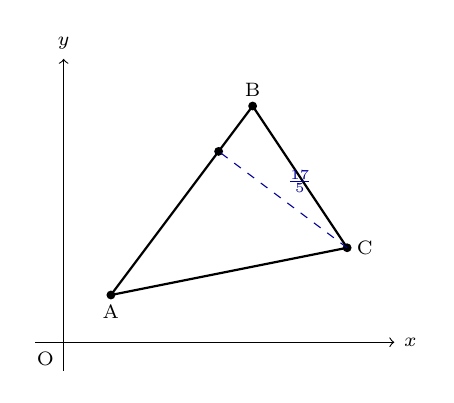
\begin{tikzpicture}[x=6mm,y=6mm]
\ax{-0.6}{7}{-0.6}{6}
\fill (1,1) circle (1.6pt);
\node[below] at (1,1){\scriptsize A};
\fill (4,5) circle (1.6pt);
\node[above] at (4,5){\scriptsize B};
\fill (6,2) circle (1.6pt);
\node[right] at (6,2){\scriptsize C};
\fill (3.28,4.04) circle (1.6pt);
\draw[thick] (1,1)--(4,5)--(6,2)--cycle; \draw[dashed,blue!60!black] (6,2)--(3.28,4.04); \node[blue!60!black] at (5.0,3.4){\tiny $\frac{17}5$};
\end{tikzpicture}
\end{center}
(1)\ $\dfrac{|3\cdot2+4\cdot3-8|}{\sqrt{3^2+4^2}}=\dfrac{|10|}5=2$\\[2pt]
(2)\ $\mathrm{AB}=\sqrt{(4-1)^2+(5-1)^2}=\sqrt{9+16}=5$\\
\hspace*{1.5em}直線 AB の傾きは $\dfrac{5-1}{4-1}=\dfrac43$ だから\quad $y-1=\dfrac43(x-1)$\\
\hspace*{1.5em}両辺に3を掛けて整理すると\quad $4x-3y-1=0$\\
\hspace*{1.5em}点 $\mathrm C(6,\ 2)$ と直線 AB の距離は\quad $\dfrac{|4\cdot6-3\cdot2-1|}{\sqrt{4^2+(-3)^2}}=\dfrac{17}5$\\
\hspace*{1.5em}面積は\quad $\dfrac12\cdot\mathrm{AB}\cdot(\text{高さ})=\dfrac12\cdot5\cdot\dfrac{17}5=\dfrac{17}2$
\end{kai}

\ans{35}{線対称}
\begin{kai}
\textbf{方針}\quad (1)は\point{AB の中点が $\ell$ 上にあり，AB $\perp\ell$}．(2)は\point{対称な点 B をとって $\mathrm{AP}=\mathrm{BP}$ に置きかえ，折れ線を1本の線分にする}．\\[2pt]
\begin{center}
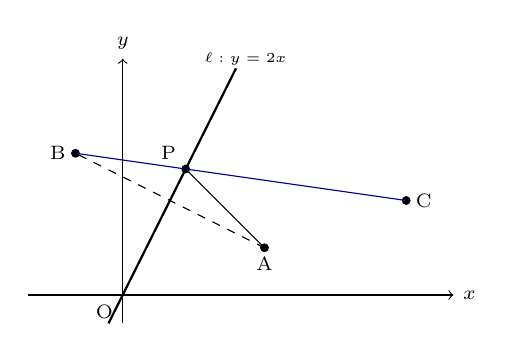
\begin{tikzpicture}[x=6mm,y=6mm]
\ax{-2}{7}{-0.6}{5}
\draw[thick,domain=-0.3:2.4,samples=80] plot (\x,{2*\x});
\fill (3,1) circle (1.6pt);
\node[below] at (3,1){\scriptsize A};
\fill (-1,3) circle (1.6pt);
\node[left] at (-1,3){\scriptsize B};
\fill (6,2) circle (1.6pt);
\node[right] at (6,2){\scriptsize C};
\fill (1.3333333333333333,2.6666666666666665) circle (1.6pt);
\node[above left] at (1.3333333333333333,2.6666666666666665){\scriptsize P};
\draw[dashed] (3,1)--(-1,3); \draw[blue!60!black] (-1,3)--(6,2); \draw (3,1)--(1.333,2.667); \node at (2.6,5){\tiny $\ell:y=2x$};
\end{tikzpicture}
\end{center}
(1)\ $\mathrm B(p,\ q)$ とする．\\
\hspace*{1.5em}AB の中点 $\left(\dfrac{p+3}2,\ \dfrac{q+1}2\right)$ が $\ell$ 上にあるので\quad $\dfrac{q+1}2=2\cdot\dfrac{p+3}2$，\quad $q=2p+5$ ……①\\
\hspace*{1.5em}AB $\perp\ell$ だから，傾きの積が $-1$：\quad $\dfrac{q-1}{p-3}\cdot2=-1$，\quad $p+2q=5$ ……②\\
\hspace*{1.5em}①を②に代入して $p+4p+10=5$，$p=-1$，$q=3$．\quad $\mathrm B(-1,\ 3)$\\[2pt]
(2)\ $y-2x$ の値は A で $1-6=-5$，C で $2-12=-10$ と同符号なので，A，C は $\ell$ に関して同じ側にある．\\
\hspace*{1.5em}$\ell$ は線分 AB の垂直二等分線だから $\mathrm{AP}=\mathrm{BP}$．よって\\
\hspace*{1.5em}$\mathrm{AP}+\mathrm{PC}=\mathrm{BP}+\mathrm{PC}\geqq\mathrm{BC}=\sqrt{(6+1)^2+(2-3)^2}=\sqrt{50}=5\sqrt2$\\
\hspace*{1.5em}等号は P が線分 BC 上にあるとき（B，C は $\ell$ の反対側にあるので，BC は $\ell$ と交わる）．\\
\hspace*{1.5em}直線 BC：傾き $\dfrac{2-3}{6-(-1)}=-\dfrac17$ より $y-3=-\dfrac17(x+1)$，\quad $y=-\dfrac17x+\dfrac{20}7$\\
\hspace*{1.5em}$y=2x$ との交点：$2x=-\dfrac17x+\dfrac{20}7$，$15x=20$，$x=\dfrac43$，$y=\dfrac83$\\
\hspace*{1.5em}最小値 $5\sqrt2$，\quad そのとき\quad $\mathrm P\left(\dfrac43,\ \dfrac83\right)$
\end{kai}

\ans{36}{平行条件・垂直条件}
\begin{kai}
\textbf{方針}\quad 直線 $ax+by+c=0$ に\point{平行な直線は $a(x-x_1)+b(y-y_1)=0$，垂直な直線は $b(x-x_1)-a(y-y_1)=0$}．一般形のままなら，\point{平行 $\iff a_1b_2-a_2b_1=0$，垂直 $\iff a_1a_2+b_1b_2=0$}．\\[2pt]
\begin{center}
\begin{tikzpicture}[x=6mm,y=6mm]
\ax{-2}{4}{-1}{4.5}
\draw[thick,domain=-2:4,samples=80] plot (\x,{(2*\x+1)/3});
\draw[blue!60!black,domain=-2:4,samples=80] plot (\x,{(2*\x+4)/3});
\draw[red!70!black,domain=0.3:3,samples=80] plot (\x,{(7-3*\x)/2});
\fill (1,2) circle (1.6pt);
\node[above left] at (1,2){\scriptsize $(1,2)$};
\node at (3.6,2.2){\tiny 元の直線}; \node[blue!60!black] at (3.3,4.1){\tiny 平行}; \node[red!70!black] at (2.9,-0.6){\tiny 垂直};
\end{tikzpicture}
\end{center}
(1)\ 直線 $2x-3y+1=0$ の傾きは $\dfrac23$．\\
\hspace*{1.5em}平行な直線（傾き $\dfrac23$）：$2(x-1)-3(y-2)=0$ より\quad $2x-3y+4=0$\\
\hspace*{1.5em}垂直な直線（傾き $-\dfrac32$）：$3(x-1)+2(y-2)=0$ より\quad $3x+2y-7=0$\\[2pt]
(2)\ $a_1=a$，$b_1=2$，$a_2=1$，$b_2=a+1$．\\
\hspace*{1.5em}平行：$a(a+1)-2\cdot1=0$，\quad $a^2+a-2=0$，\quad $(a-1)(a+2)=0$ より $a=1,\ -2$\\
\hspace*{1.5em}\point{一致する場合を除く}：$a=1$ のとき $x+2y=1$ と $x+2y=3$，$a=-2$ のとき $-2x+2y=1$ と $x-y=3$．\\
\hspace*{1.5em}どちらも一致しないので\quad $a=1,\ -2$\\[2pt]
\hspace*{1.5em}垂直：$a\cdot1+2(a+1)=0$，\quad $3a+2=0$ より\quad $a=-\dfrac23$
\end{kai}

\ans{37}{定点を通る直線}
\begin{kai}
\textbf{方針}\quad \point{$k$ について整理して，$k\times(\ \ )+(\ \ )=0$ の形にする}．これが $k$ の恒等式となる条件は，両方のかっこが0．\\[2pt]
与式を展開して $k$ について整理すると\\
\hspace*{1.5em}$2kx+x+ky-y-4k+1=0$，\quad $k(2x+y-4)+(x-y+1)=0$\\[2pt]
これがすべての $k$ で成りたつ条件は\quad $2x+y-4=0$ かつ $x-y+1=0$\\
2式を加えて $3x-3=0$，$x=1$．よって $y=2$．\\[2pt]
定点は\quad $(1,\ 2)$
\begin{center}
\begin{tikzpicture}[x=6mm,y=6mm]
\ax{-1.5}{3.5}{-1}{5}
\draw[thick,domain=-1.5:3.5,samples=80] plot (\x,{\x+1});
\draw[thick,domain=0:2.5,samples=80] plot (\x,{4-2*\x});
\draw[thick,domain=-1.5:3.5,samples=80] plot (\x,{(\x+5)/2});
\draw[gray,domain=-1.5:3.5,samples=80] plot (\x,{-0.5*\x+2.5});
\fill (1,2) circle (1.6pt);
\node[below right] at (1,2){\scriptsize $(1,2)$};
\draw (1,-1)--(1,5);
\node[below] at (current bounding box.south){\scriptsize $k$ を変えても，すべて点 $(1,2)$ を通る};
\end{tikzpicture}
\end{center}
\end{kai}

\ans{38}{交点を通る直線}
\begin{kai}
\textbf{方針}\quad 2直線 $f=0$，$g=0$ の交点を通る直線は\point{$f+kg=0$（$k$ は定数）}と表せる（ただし $g=0$ 自身は表せない）．交点を求めずに済む．\\[2pt]
\begin{center}
\begin{tikzpicture}[x=6mm,y=6mm]
\ax{-1}{4}{-1.5}{4.5}
\draw[gray,domain=-0.2:2.7,samples=80] plot (\x,{4-2*\x});
\draw[gray,domain=-1:3.3,samples=80] plot (\x,{\x+1});
\draw[thick,blue!60!black,domain=-1:4,samples=80] plot (\x,{3-\x});
\fill (1,2) circle (1.6pt);
\node[above right] at (1,2){\scriptsize 交点 $(1,2)$};
\fill (3,0) circle (1.6pt);
\node[below] at (3,0){\scriptsize $(3,0)$};
\end{tikzpicture}
\end{center}
求める直線は\quad $(2x+y-4)+k(x-y+1)=0$ ……① とおける．\\
（$x-y+1=0$ 自身は $(3,\ 0)$ を通らないので，この形で表せないものを考えなくてよい．）\\[2pt]
①が点 $(3,\ 0)$ を通るので\quad $(6+0-4)+k(3-0+1)=0$，\quad $2+4k=0$，\quad $k=-\dfrac12$\\
①に代入して\quad $(2x+y-4)-\dfrac12(x-y+1)=0$\\
両辺を2倍して $4x+2y-8-x+y-1=0$，\quad $3x+3y-9=0$．\quad よって\quad $x+y-3=0$\\[2pt]
（確認：2直線の交点は $(1,\ 2)$ で，$1+2-3=0$．$(3,\ 0)$ も $3+0-3=0$ をみたす．）
\end{kai}

\ans{39}{円の方程式}
\begin{kai}
\textbf{方針}\quad 中心と半径がわかれば\point{$(x-a)^2+(y-b)^2=r^2$}．3点を通る円は\point{$x^2+y^2+lx+my+n=0$ とおいて代入}．一般形が円を表すかは平方完成して右辺 $>0$ を調べる．\\[2pt]
(1)\ 半径は中心 $(2,\ -1)$ と点 $(5,\ 3)$ の距離で\quad $\sqrt{(5-2)^2+(3+1)^2}=\sqrt{9+16}=5$\\
\hspace*{1.5em}$(x-2)^2+(y+1)^2=25$\\[2pt]
(2)\ $x^2+y^2+lx+my+n=0$ に3点を代入すると\\
\hspace*{1.5em}$(0,\ 0)$：$n=0$，\quad $(4,\ 0)$：$16+4l+n=0$，\quad $(0,\ 2)$：$4+2m+n=0$\\
\hspace*{1.5em}よって $n=0$，$l=-4$，$m=-2$．\quad $x^2+y^2-4x-2y=0$\\
\hspace*{1.5em}平方完成すると $(x-2)^2+(y-1)^2=5$ より\quad 中心 $(2,\ 1)$，半径 $\sqrt5$\\
\hspace*{1.5em}（3点のうち $(4,\ 0)$ と $(0,\ 2)$ を結ぶ線分は，原点で直角をはさむので直径になっている．）\\[2pt]
(3)\ 平方完成すると\quad $(x-3)^2-9+(y+2)^2-4+k=0$，\quad $(x-3)^2+(y+2)^2=13-k$\\
\begin{center}
\begin{tikzpicture}[x=3mm,y=3mm]
\draw[dashed] (2,-1)--(5,3);
\ax{-4}{8.5}{-6.5}{5}
\fill (2,-1) circle (1.6pt);
\node[below] at (2,-1){\scriptsize 中心};
\fill (5,3) circle (1.6pt);
\node[right] at (5,3){\scriptsize $(5,3)$};
\draw[thick] (2,-1) circle (5);
\node[below] at (current bounding box.south){\scriptsize (1)};
\end{tikzpicture}\hspace{1.2em}
\begin{tikzpicture}[x=6mm,y=6mm]
\draw[dashed] (4,0)--(0,2);
\ax{-1}{5}{-0.8}{4}
\fill (0,0) circle (1.6pt);
\fill (4,0) circle (1.6pt);
\node[below right] at (4,0){\scriptsize 4};
\fill (0,2) circle (1.6pt);
\node[left] at (0,2){\scriptsize 2};
\fill (2,1) circle (1.6pt);
\node[right] at (2,1){\scriptsize 中心};
\draw[thick] (2,1) circle (2.236);
\node[below] at (current bounding box.south){\scriptsize (2) 直径の両端は $(4,0),(0,2)$};
\end{tikzpicture}
\end{center}
\hspace*{1.5em}円を表すのは右辺が正のときだから\quad $13-k>0$，\quad $k<13$\\
\hspace*{1.5em}（$k=13$ なら点 $(3,\ -2)$ だけ，$k>13$ なら図形を表さない．）
\end{kai}

\ans{40}{円と直線の位置関係}
\begin{kai}
\textbf{方針}\quad 円と直線の位置関係は\point{中心と直線の距離 $d$ と半径 $r$ を比べる}：$d<r$ で2個，$d=r$ で1個（接する），$d>r$ で0個．弦の長さは三平方の定理．\\[2pt]
(1)\ 円の中心は原点，半径は $\sqrt5$．直線 $2x-y+k=0$ と原点の距離は\\
\hspace*{1.5em}$d=\dfrac{|2\cdot0-0+k|}{\sqrt{2^2+(-1)^2}}=\dfrac{|k|}{\sqrt5}$\\[2pt]
\hspace*{1.5em}$d<\sqrt5$，すなわち $|k|<5$（$-5<k<5$）のとき\quad 共有点は2個\\
\hspace*{1.5em}$d=\sqrt5$，すなわち $|k|=5$（$k=\pm5$）のとき\quad 共有点は1個\\
\hspace*{1.5em}$d>\sqrt5$，すなわち $|k|>5$（$k<-5,\ 5<k$）のとき\quad 共有点は0個\\
\begin{center}
\begin{tikzpicture}[x=5mm,y=5mm]
\ax{-3}{3}{-3}{3.5}
\draw[blue!60!black,domain=-2.6:0.75,samples=80] plot (\x,{2*\x+2});
\draw[thick] (0,0) circle (2.236);
\node[below] at (current bounding box.south){\scriptsize $|k|<5$：2個};
\end{tikzpicture}\hspace{1.2em}
\begin{tikzpicture}[x=5mm,y=5mm]
\ax{-3}{3}{-3}{3.5}
\draw[blue!60!black,domain=-4.1:-0.75,samples=80] plot (\x,{2*\x+5});
\draw[thick] (0,0) circle (2.236);
\fill (-2,1) circle (1.6pt); \node[left] at (-2,1){\tiny 接点};\node[below] at (current bounding box.south){\scriptsize $|k|=5$：1個};
\end{tikzpicture}\hspace{1.2em}
\begin{tikzpicture}[x=5mm,y=5mm]
\ax{-3}{3}{-3}{3.5}
\draw[blue!60!black,domain=-5.1:-1.75,samples=80] plot (\x,{2*\x+7});
\draw[thick] (0,0) circle (2.236);
\node[below] at (current bounding box.south){\scriptsize $|k|>5$：0個};
\end{tikzpicture}
\end{center}
\hspace*{1.5em}（判別式でもよい：$x^2+(2x+k)^2=5$，$5x^2+4kx+k^2-5=0$ の $\dfrac D4=4k^2-5(k^2-5)=25-k^2$．）\\[2pt]
(2)\ $k=\sqrt5$ のとき $d=\dfrac{\sqrt5}{\sqrt5}=1$．\\
\hspace*{1.5em}中心から弦に下ろした垂線は弦を2等分する．弦の長さの半分を $l$ とすると，三平方の定理より\\
\begin{center}
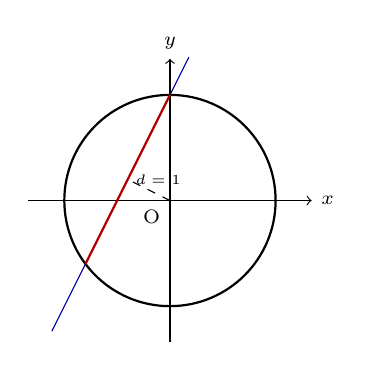
\begin{tikzpicture}[x=6mm,y=6mm]
\ax{-3}{3}{-3}{3}
\draw[blue!60!black,domain=-2.5:0.4,samples=80] plot (\x,{2*\x+2.236});
\draw[thick] (0,0) circle (2.236);\draw[dashed] (0,0)--(-0.894,0.447); \node at (-0.25,0.45){\tiny $d=1$}; \draw[thick,red!70!black] (-1.788,-1.342)--(0,2.236);
\end{tikzpicture}
\end{center}
\hspace*{1.5em}$l^2+d^2=r^2$，\quad $l=\sqrt{5-1}=2$．\quad 弦の長さは\quad $2l=4$
\end{kai}

\ans{41}{円と接線}
\begin{kai}
\textbf{方針}\quad \point{円 $x^2+y^2=r^2$ 上の点 $(x_1,\ y_1)$ における接線は $x_1x+y_1y=r^2$}．円外の点からの接線は，\point{接点を $(x_1,\ y_1)$ とおいて}この公式を使う．\\[2pt]
(1)\ 点 $(1,\ 2)$ は $1^2+2^2=5$ より円上の点．接線は\quad $1\cdot x+2\cdot y=5$，すなわち\quad $x+2y=5$\\[2pt]
(2)\ 接点を $(x_1,\ y_1)$ とすると，$x_1^2+y_1^2=5$ ……①，接線は $x_1x+y_1y=5$ ……②．\\
\hspace*{1.5em}②が点 $(5,\ 0)$ を通るので\quad $5x_1=5$，\quad $x_1=1$\\
\hspace*{1.5em}①に代入して $1+y_1^2=5$，\quad $y_1=\pm2$\\
\hspace*{1.5em}$y_1=2$ のとき\quad 接線 $x+2y=5$，接点 $(1,\ 2)$\\
\hspace*{1.5em}$y_1=-2$ のとき\quad 接線 $x-2y=5$，接点 $(1,\ -2)$\\
\hspace*{1.5em}（別解：接線を $y=m(x-5)$ とおき，中心との距離 $=$ 半径 から $m=\pm\dfrac12$ を求めてもよい．）
\begin{center}
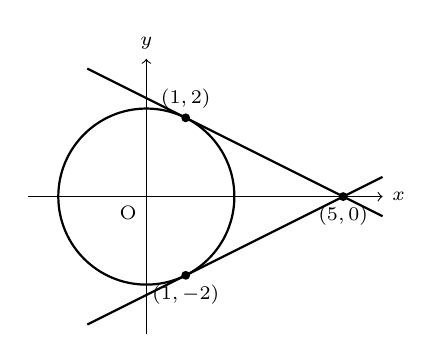
\begin{tikzpicture}[x=5mm,y=5mm]
\ax{-3}{6}{-3.5}{3.5}
\draw[thick,domain=-1.5:6,samples=80] plot (\x,{(5-\x)/2});
\draw[thick,domain=-1.5:6,samples=80] plot (\x,{(\x-5)/2});
\fill (5,0) circle (1.6pt);
\node[below] at (5,0){\scriptsize $(5,0)$};
\fill (1,2) circle (1.6pt);
\node[above] at (1,2){\scriptsize $(1,2)$};
\fill (1,-2) circle (1.6pt);
\node[below] at (1,-2){\scriptsize $(1,-2)$};
\draw[thick] (0,0) circle (2.236);
\end{tikzpicture}
\end{center}
\end{kai}

\ans{42}{2円の交点を通る円}
\begin{kai}
\textbf{方針}\quad 2円 $f=0$，$g=0$ の交点を通る図形は\point{$f+kg=0$} と表せる．$k=-1$ なら2次の項が消えて直線，それ以外は円．\\[2pt]
（2円の中心は $(0,\ 0)$ と $(2,\ 1)$ で距離 $\sqrt5$，半径は3と $\sqrt6$．$3-\sqrt6<\sqrt5<3+\sqrt6$ だから2点で交わる．）\\[2pt]
(1)\ $(x^2+y^2-9)+k(x^2+y^2-4x-2y-1)=0$ で $k=-1$ とすると\\
\hspace*{1.5em}$(x^2+y^2-9)-(x^2+y^2-4x-2y-1)=0$，\quad $4x+2y-8=0$．すなわち\quad $2x+y-4=0$\\
\hspace*{1.5em}（2つの交点はどちらも両方の円の式をみたすので，差の式もみたす．）\\[2pt]
(2)\ $(x^2+y^2-9)+k(x^2+y^2-4x-2y-1)=0$ ……① が原点を通るので\\
\hspace*{1.5em}$-9+k\cdot(-1)=0$，\quad $k=-9$\\
\hspace*{1.5em}①に代入して $(x^2+y^2-9)-9(x^2+y^2-4x-2y-1)=0$，\quad $-8x^2-8y^2+36x+18y=0$\\
\hspace*{1.5em}両辺を $-8$ で割って\quad $x^2+y^2-\dfrac92x-\dfrac94y=0$
\begin{center}
\begin{tikzpicture}[x=5mm,y=5mm]
\ax{-3.5}{5}{-3.5}{4}
\draw[red!70!black,domain=0.2:3.5,samples=80] plot (\x,{4-2*\x});
\draw[gray] (0,0) circle (3);\draw[gray] (2,1) circle (2.449);\draw[thick,blue!60!black] (2.25,1.125) circle (2.516);
\node[below] at (current bounding box.south){\scriptsize 灰色：もとの2円，赤：(1)の直線，青：(2)の円};
\end{tikzpicture}
\end{center}
\end{kai}

\ans{43}{軌跡（Ⅰ）}
\begin{kai}
\textbf{方針}\quad 軌跡は\point{動く点を $(x,\ y)$ とおき，条件を $x,\ y$ の式で表す}．距離の条件は2乗して根号を消す．\\[2pt]
$\mathrm P(x,\ y)$ とする．$\mathrm{AP}:\mathrm{BP}=2:1$ より $\mathrm{AP}=2\mathrm{BP}$．両辺を2乗して $\mathrm{AP}^2=4\mathrm{BP}^2$\\
\hspace*{1.5em}$x^2+y^2=4\{(x-3)^2+y^2\}$\\
\hspace*{1.5em}$x^2+y^2=4x^2-24x+36+4y^2$，\quad $3x^2+3y^2-24x+36=0$\\
\hspace*{1.5em}$x^2+y^2-8x+12=0$，\quad $(x-4)^2+y^2=4$\\[2pt]
逆に，この円上の点はすべて条件をみたす．\\
よって軌跡は\quad 中心 $(4,\ 0)$，半径2の円\quad（アポロニウスの円）\\
（この円は AB を $2:1$ に内分する点 $(2,\ 0)$ と外分する点 $(6,\ 0)$ を直径の両端とする．）
\begin{center}
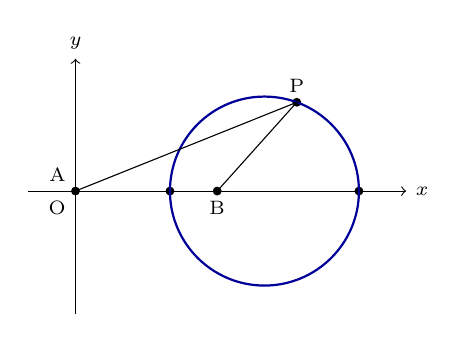
\begin{tikzpicture}[x=6mm,y=6mm]
\ax{-1}{7}{-2.6}{2.8}
\fill (0,0) circle (1.6pt);
\node[above left] at (0,0){\scriptsize A};
\fill (3,0) circle (1.6pt);
\node[below] at (3,0){\scriptsize B};
\fill (2,0) circle (1.6pt);
\fill (6,0) circle (1.6pt);
\fill (4.684040286651338,1.8793852415718166) circle (1.6pt);
\node[above] at (4.684040286651338,1.8793852415718166){\scriptsize P};
\draw[thick,blue!60!black] (4,0) circle (2);\draw (0,0)--(4.684,1.879)--(3,0);
\end{tikzpicture}
\end{center}
\end{kai}

\ans{44}{軌跡（Ⅱ）}
\begin{kai}
\textbf{方針}\quad \point{動く点 Q の座標を $s,\ t$，軌跡を求める点 M を $(x,\ y)$ とし，$s,\ t$ を $x,\ y$ で表して Q の条件式に代入}する．\\[2pt]
$\mathrm Q(s,\ t)$，$\mathrm M(x,\ y)$ とする．Q は円上にあるので\quad $s^2+t^2=4$ ……①\\
M は AQ の中点だから\quad $x=\dfrac{s+4}2$，\quad $y=\dfrac{t+0}2$\\
よって\quad $s=2x-4$，\quad $t=2y$\\[2pt]
①に代入して\quad $(2x-4)^2+(2y)^2=4$\\
両辺を4で割って\quad $(x-2)^2+y^2=1$\\[2pt]
軌跡は\quad 中心 $(2,\ 0)$，半径1の円\\
\begin{center}
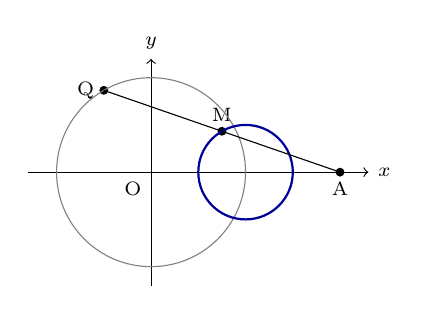
\begin{tikzpicture}[x=6mm,y=6mm]
\ax{-2.6}{4.6}{-2.4}{2.4}
\fill (4,0) circle (1.6pt);
\node[below] at (4,0){\scriptsize A};
\fill (-0.9999999999999996,1.7320508075688774) circle (1.6pt);
\node[left] at (-0.9999999999999996,1.7320508075688774){\scriptsize Q};
\fill (1.5000000000000002,0.8660254037844387) circle (1.6pt);
\node[above] at (1.5000000000000002,0.8660254037844387){\scriptsize M};
\draw[gray] (0,0) circle (2);\draw[thick,blue!60!black] (2,0) circle (1);\draw (-1.000,1.732)--(4,0);
\end{tikzpicture}
\end{center}
（もとの円を A を中心に $\dfrac12$ 倍に縮小した円になっている．）
\end{kai}

\ans{45}{軌跡（Ⅲ）}
\begin{kai}
\textbf{方針}\quad 頂点の座標を $t$ で表し，\point{$x=(t\text{の式})$，$y=(t\text{の式})$ から $t$ を消去}する．$t$ の動く範囲から $x$ の範囲も確認する．\\[2pt]
$y=x^2-2tx+3t=(x-t)^2-t^2+3t$\\
よって頂点は\quad $(t,\ -t^2+3t)$\\[2pt]
頂点を $(x,\ y)$ とすると\quad $x=t$，\quad $y=-t^2+3t$\\
$t=x$ を代入して $t$ を消去すると\quad $y=-x^2+3x$\\
$t$ は実数全体を動くので，$x$ も実数全体を動く（除く部分はない）．\\[2pt]
軌跡は\quad 放物線\quad $y=-x^2+3x$
\begin{center}
\begin{tikzpicture}[x=6mm,y=6mm]
\ax{-1.5}{4}{-1}{3}
\draw[gray,domain=-1:1,samples=80] plot (\x,{(\x-0)^2-(0)^2+3*(0)});
\draw[gray,domain=-0.25:1.75,samples=80] plot (\x,{(\x-0.75)^2-(0.75)^2+3*(0.75)});
\draw[gray,domain=0.5:2.5,samples=80] plot (\x,{(\x-1.5)^2-(1.5)^2+3*(1.5)});
\draw[gray,domain=1.25:3.25,samples=80] plot (\x,{(\x-2.25)^2-(2.25)^2+3*(2.25)});
\draw[gray,domain=2:4,samples=80] plot (\x,{(\x-3)^2-(3)^2+3*(3)});
\draw[thick,blue!60!black,domain=-0.3:3.3,samples=80] plot (\x,{-(\x)^2+3*\x});
\fill (0,0) circle (1.6pt);
\fill (0.75,1.6875) circle (1.6pt);
\fill (1.5,2.25) circle (1.6pt);
\fill (2.25,1.6875) circle (1.6pt);
\fill (3,0) circle (1.6pt);
\node[below] at (current bounding box.south){\scriptsize 灰色：$t$ を変えたときの放物線，青：頂点の軌跡};
\end{tikzpicture}
\end{center}
\end{kai}

\ans{46}{軌跡（Ⅳ）}
\begin{kai}
\textbf{方針}\quad 交点 $(x,\ y)$ の2式から\point{パラメータ $m$ を消去}する．$m$ について解くときに割る数が0になる場合を確かめ，\point{除外点}に注意する．\\[2pt]
交点を $(x,\ y)$ とすると\quad $y=mx$ ……①，\quad $x+my=2$ ……②\\[2pt]
$x=0$ とすると，①より $y=0$ となり，②は $0=2$ で成りたたない．よって $x\neq0$．\\
①より $m=\dfrac yx$．②に代入して\quad $x+\dfrac{y^2}x=2$，\quad $x^2+y^2=2x$，\quad $(x-1)^2+y^2=1$\\[2pt]
逆に，この円上の $x\neq0$ である点 $(x,\ y)$ に対して $m=\dfrac yx$ とおけば①②をみたす．\\
円 $(x-1)^2+y^2=1$ 上で $x=0$ となる点は原点だけ．\\[2pt]
\point{除外点に注意}．軌跡は\quad 円 $(x-1)^2+y^2=1$ から原点 $(0,\ 0)$ を除いた部分\\
\begin{center}
\begin{tikzpicture}[x=12mm,y=12mm]
\ax{-0.8}{3}{-1.5}{1.5}
\draw[gray,domain=-0.5:2.6,samples=80] plot (\x,{0.5*\x});
\draw[gray,domain=1.3:2.6,samples=80] plot (\x,{(2-\x)/0.5});
\fill (1.6,0.8) circle (1.6pt);
\node[above] at (1.6,0.8){\scriptsize 交点};
\draw[thick,blue!60!black] (1,0) circle (1);\draw[fill=white] (0,0) circle (2pt);
\node[below] at (current bounding box.south){\scriptsize 白丸の原点は除く};
\end{tikzpicture}
\end{center}
（原点は，直線 $x+my=2$ が原点を通らないことからも除かれる．）
\end{kai}

\ans{47}{軌跡（Ⅴ）}
\begin{kai}
\textbf{方針}\quad 交点の $x$ 座標は連立した2次方程式の解 $\alpha,\ \beta$．\point{中点の座標を解と係数の関係で $m$ の式に}し，$m$ を消去する．\point{「異なる2点で交わる」条件から $x$ の範囲}が出る．\\[2pt]
直線は $y=m(x-3)$．$y=x^2$ と連立して $x^2=m(x-3)$，\quad $x^2-mx+3m=0$ ……①\\
異なる2点で交わる条件は①の判別式 $D>0$：$m^2-12m>0$，\quad $m(m-12)>0$ より\quad $m<0,\ 12<m$\\[2pt]
①の2解を $\alpha,\ \beta$ とすると，解と係数の関係より $\alpha+\beta=m$．\\
中点を $(X,\ Y)$ とすると\quad $X=\dfrac{\alpha+\beta}2=\dfrac m2$\\
中点は直線上にあるので\quad $Y=m(X-3)$\\[2pt]
$m=2X$ を代入して\quad $Y=2X(X-3)=2X^2-6X$\\
$m<0,\ 12<m$ より\quad $X<0,\ 6<X$\\[2pt]
軌跡は\quad 放物線 $y=2x^2-6x$ の $x<0,\ 6<x$ の部分
\begin{center}
\begin{tikzpicture}[x=6mm,y=3mm]
\ax{-3}{4}{-1}{10}
\draw[thick,domain=-3:3.1,samples=80] plot (\x,{(\x)^2});
\draw[gray,domain=-2.8:3.6,samples=80] plot (\x,{-(\x-3)});
\draw[thick,blue!60!black,dashed,domain=-1.3:0,samples=80] plot (\x,{2*(\x)^2-6*\x});
\fill (3,0) circle (1.6pt);
\node[below] at (3,0){\scriptsize $(3,0)$};
\fill (-2.303,5.303) circle (1.6pt);
\fill (1.303,1.697) circle (1.6pt);
\fill (-0.5,3.5) circle (1.6pt);
\node[left] at (-0.5,3.5){\scriptsize 中点};
\node[below] at (current bounding box.south){\scriptsize 青の点線：中点の軌跡（$x<0$ の部分．$x>6$ の部分は図の外）};
\end{tikzpicture}
\end{center}
\end{kai}

\ans{48}{一般の曲線の移動}
\begin{kai}
\textbf{方針}\quad 曲線 $f(x,\ y)=0$ の移動は，\point{移動後の点 $(x,\ y)$ のもとの点を求め，それを $f$ に代入}する．平行移動なら $x\to x-p$，$y\to y-q$．\\[2pt]
(1)\ 移動後の点 $(x,\ y)$ のもとの点は $(x-3,\ y+1)$．これが $C$ 上にあるので\\
\hspace*{1.5em}\point{$x$ を $x-3$，$y$ を $y+1$ におきかえる}\\
\hspace*{1.5em}$y+1=(x-3)^2-2(x-3)=x^2-6x+9-2x+6=x^2-8x+15$\\
\hspace*{1.5em}よって\quad $y=x^2-8x+14$\\
\hspace*{1.5em}（確認：$C$ の頂点 $(1,\ -1)$ は $(4,\ -2)$ に移り，$y=(x-4)^2-2=x^2-8x+14$ と一致．）\\[2pt]
(2)\ 点 $(x,\ y)$ と点 $(1,\ 1)$ に関して対称な点を $(X,\ Y)$ とすると，$(1,\ 1)$ が中点だから\\
\hspace*{1.5em}$\dfrac{x+X}2=1$，$\dfrac{y+Y}2=1$ より\quad $X=2-x$，$Y=2-y$\\
\hspace*{1.5em}$(X,\ Y)$ が $C$ 上にあるので\quad $2-y=(2-x)^2-2(2-x)=x^2-2x$\\
\hspace*{1.5em}よって\quad $y=-x^2+2x+2$
\begin{center}
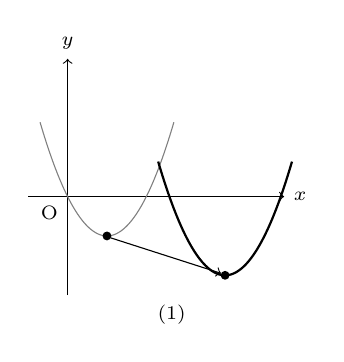
\begin{tikzpicture}[x=5mm,y=5mm]
\ax{-1}{5.5}{-2.5}{3.5}
\draw[gray,domain=-0.7:2.7,samples=80] plot (\x,{(\x)^2-2*\x});
\draw[thick,domain=2.3:5.7,samples=80] plot (\x,{(\x)^2-8*\x+14});
\fill (1,-1) circle (1.6pt);
\fill (4,-2) circle (1.6pt);
\draw[->] (1.1,-1.05)--(3.9,-1.95);
\node[below] at (current bounding box.south){\scriptsize (1)};
\end{tikzpicture}\hspace{1.2em}
\begin{tikzpicture}[x=5mm,y=5mm]
\ax{-1.5}{3.5}{-2}{4}
\draw[gray,domain=-0.7:2.7,samples=80] plot (\x,{(\x)^2-2*\x});
\draw[thick,domain=-0.7:2.7,samples=80] plot (\x,{-(\x)^2+2*\x+2});
\fill (1,1) circle (1.6pt);
\node[right] at (1,1){\scriptsize $(1,1)$};
\node[below] at (current bounding box.south){\scriptsize (2) 点 $(1,1)$ に関して対称};
\end{tikzpicture}
\end{center}
\end{kai}

\ans{49}{不等式の表す領域（Ⅰ）}
\begin{kai}
\textbf{方針}\quad \point{$y>f(x)$ は曲線 $y=f(x)$ の上側，$y<f(x)$ は下側}．それぞれの領域を求め，共通部分をとる．境界線の交点も求める．\\[2pt]
\begin{minipage}[t]{0.55\linewidth}
放物線 $y=x^2-2$ の上側と，直線 $y=x$ の下側の共通部分．\\
交点は $x^2-2=x$ より $x=-1,\ 2$，すなわち $(-1,\ -1)$，$(2,\ 2)$．\\
右図の斜線部分．境界線を含む．
\end{minipage}\hfill
\begin{minipage}[t]{0.4\linewidth}
\vspace{-6pt}
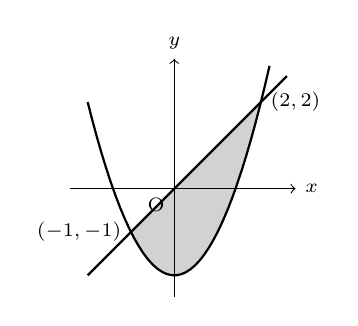
\begin{tikzpicture}[scale=0.55]
\fill[gray!35] plot[domain=-1:2,samples=40] (\x,{\x*\x-2}) -- (2,2) -- (-1,-1) -- cycle;
\ax{-2.4}{2.8}{-2.5}{3}
\draw[thick,domain=-2:2.2,samples=40] plot (\x,{\x*\x-2});
\draw[thick] (-2,-2)--(2.6,2.6);
\node[right] at (2,2){\scriptsize $(2,2)$}; \node[left] at (-1,-1){\scriptsize $(-1,-1)$};
\end{tikzpicture}
\end{minipage}
\end{kai}

\ans{50}{不等式の表す領域（Ⅱ）}
\begin{kai}
\textbf{方針}\quad \point{$AB>0\iff$「$A>0$ かつ $B>0$」または「$A<0$ かつ $B<0$」}．2直線で平面が4つに分かれ，そのうち向かいあう2つの部分が答え．\\[2pt]
\begin{minipage}[t]{0.55\linewidth}
\point{積が正 $\iff$ 2因数が同符号}\\
$x-y>0\iff y<x$，\quad $x+y-2>0\iff y>-x+2$ だから\\
「$y<x$ かつ $y>-x+2$」または「$y>x$ かつ $y<-x+2$」．\\
2直線 $y=x$，$y=-x+2$ は点 $(1,\ 1)$ で交わる．\\
右図の斜線部分．境界線を含まない．
\end{minipage}\hfill
\begin{minipage}[t]{0.4\linewidth}
\vspace{-6pt}
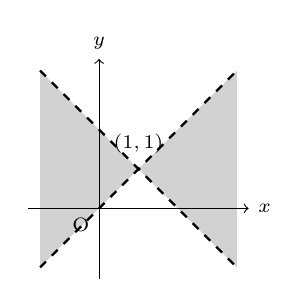
\begin{tikzpicture}[scale=0.5]
\fill[gray!35] (1,1)--(3.5,3.5)--(3.5,-1.5)--cycle;
\fill[gray!35] (1,1)--(-1.5,-1.5)--(-1.5,3.5)--cycle;
\ax{-1.8}{3.8}{-1.8}{3.8}
\draw[thick,dashed] (-1.5,-1.5)--(3.5,3.5); \draw[thick,dashed] (-1.5,3.5)--(3.5,-1.5);
\node[above] at (1,1.15){\scriptsize $(1,1)$};
\end{tikzpicture}
\end{minipage}
\end{kai}

\ans{51}{領域内の点に対する最大・最小}
\begin{kai}
\textbf{方針}\quad まず領域を図示する．$x+y=k$ は\point{直線とみて，領域と共有点をもつ範囲で $k$ を動かす}．$x^2+y^2$ は\point{原点からの距離の2乗}とみる．\\[2pt]
$x+2y=8$ と $3x+y=9$ の交点：第2式より $y=9-3x$，第1式に代入して $x+18-6x=8$，$x=2$，$y=3$．\\
領域は4点 $(0,0)$，$(3,0)$，$(2,3)$，$(0,4)$ を頂点とする四角形の周および内部．\\[2pt]
(1)\ $x+y=k$ とおくと $y=-x+k$ で，傾き $-1$，$y$ 切片 $k$ の直線．\\
\begin{center}
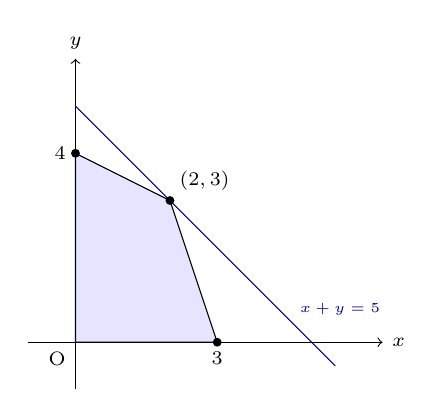
\begin{tikzpicture}[x=6mm,y=6mm]
\fill[blue!10] (0,0)--(3,0)--(2,3)--(0,4)--cycle;
\ax{-1}{6.5}{-1}{6}
\draw[blue!60!black,domain=0:5.5,samples=80] plot (\x,{5-\x});
\fill (2,3) circle (1.6pt);
\node[above right] at (2,3){\scriptsize $(2,3)$};
\fill (3,0) circle (1.6pt);
\node[below] at (3,0){\scriptsize 3};
\fill (0,4) circle (1.6pt);
\node[left] at (0,4){\scriptsize 4};
\draw (0,0)--(3,0)--(2,3)--(0,4)--cycle; \node[blue!60!black] at (5.6,0.7){\tiny $x+y=5$};
\end{tikzpicture}
\end{center}
\hspace*{1.5em}この直線が領域と共有点をもつときの $k$ の最大値を考える．\\
\hspace*{1.5em}境界の傾きは $x+2y=8$ が $-\dfrac12$，$3x+y=9$ が $-3$ で，$-3<-1<-\dfrac12$ だから，\\
\hspace*{1.5em}$y$ 切片が最大になるのは直線が頂点 $(2,\ 3)$ を通るとき．\\
\hspace*{1.5em}最大値 $2+3=5$\quad（$x=2$，$y=3$）\\
\hspace*{1.5em}（各頂点での値 0，3，5，4 を比べても確かめられる．）\\[2pt]
(2)\ $x^2+y^2=r^2$ とおくと，これは原点を中心とする半径 $r$ の円．$r$ は原点から点 $(x,\ y)$ までの距離．\\
\begin{center}
\begin{tikzpicture}[x=6mm,y=6mm]
\fill[blue!10] (0,0)--(3,0)--(2,3)--(0,4)--cycle;
\ax{-1}{5}{-1}{5}
\fill (0,4) circle (1.6pt);
\node[above right] at (0,4){\scriptsize $(0,4)$};
\draw (0,0)--(3,0)--(2,3)--(0,4)--cycle; \draw[red!70!black] (4,0) arc (0:90:4);
\node[below] at (current bounding box.south){\scriptsize 原点中心の円が領域と共有点をもつ範囲};
\end{tikzpicture}
\end{center}
\hspace*{1.5em}最大：原点から最も遠い点は頂点のどれか．$(3,0)$：9，$(2,3)$：13，$(0,4)$：16．\\
\hspace*{1.5em}\quad 最大値 $16$\quad（$x=0$，$y=4$）\\
\hspace*{1.5em}最小：原点は領域に含まれるので\quad 最小値 $0$\quad（$x=0$，$y=0$）
\end{kai}

\shouans{第4章}{三角関数}
\ans{52}{一般角}
\begin{kai}
\textbf{方針}\quad \point{$360^\circ$ を何回分引けば（足せば）$0^\circ$〜$360^\circ$ に入るか}を考える．$\alpha$ の大きさで象限がわかる．\\[2pt]
\begin{center}
\begin{tikzpicture}[scale=1,x=12mm,y=12mm]
\draw[->] (-1.35,0)--(1.4,0) node[right]{\tiny $x$}; \draw[->] (0,-1.35)--(0,1.4) node[above]{\tiny $y$}; \draw[gray] (0,0) circle (1); \node[below left] at (0,0){\tiny O};\draw[] (0.000,0.000)--(0.766,0.643);\fill (0.766,0.643) circle (1.4pt);\draw[->,blue!60!black] (0:0.25) arc (0:400:0.25);\node at (0.55,0.15){\tiny $40^\circ$};\node[below] at (current bounding box.south){\scriptsize (1) $400^\circ$：1周＋$40^\circ$};
\end{tikzpicture}\hspace{1.2em}
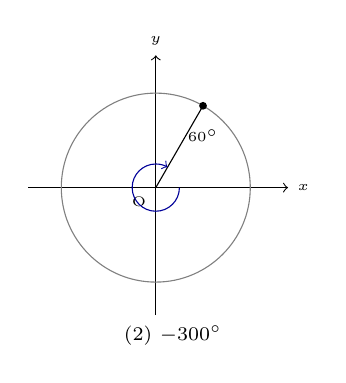
\begin{tikzpicture}[scale=1,x=12mm,y=12mm]
\draw[->] (-1.35,0)--(1.4,0) node[right]{\tiny $x$}; \draw[->] (0,-1.35)--(0,1.4) node[above]{\tiny $y$}; \draw[gray] (0,0) circle (1); \node[below left] at (0,0){\tiny O};\draw[] (0.000,0.000)--(0.500,0.866);\fill (0.500,0.866) circle (1.4pt);\draw[->,blue!60!black] (0:0.25) arc (0:-300:0.25);\node at (0.5,0.55){\tiny $60^\circ$};\node[below] at (current bounding box.south){\scriptsize (2) $-300^\circ$};
\end{tikzpicture}\hspace{1.2em}
\begin{tikzpicture}[scale=1,x=12mm,y=12mm]
\draw[->] (-1.35,0)--(1.4,0) node[right]{\tiny $x$}; \draw[->] (0,-1.35)--(0,1.4) node[above]{\tiny $y$}; \draw[gray] (0,0) circle (1); \node[below left] at (0,0){\tiny O};\draw[] (0.000,0.000)--(0.174,-0.985);\fill (0.174,-0.985) circle (1.4pt);\draw[->,blue!60!black,thin] (0:0.12) arc (0:1000:0.12);\node at (0.45,-0.65){\tiny $280^\circ$};\node[below] at (current bounding box.south){\scriptsize (3) $1000^\circ$：2周＋$280^\circ$};
\end{tikzpicture}
\end{center}
(1)\ $400^\circ=40^\circ+360^\circ$ より\quad $40^\circ+360^\circ\times1$．\quad $0^\circ<40^\circ<90^\circ$ だから\quad 第1象限\\[2pt]
(2)\ $-300^\circ=60^\circ-360^\circ$ より\quad $60^\circ+360^\circ\times(-1)$．\quad 第1象限\\
\hspace*{1.5em}（時計回りに $300^\circ$ 回ると，反時計回りに $60^\circ$ 回ったのと同じ位置）\\[2pt]
(3)\ $1000^\circ=280^\circ+720^\circ$ より\quad $280^\circ+360^\circ\times2$．\quad $270^\circ<280^\circ<360^\circ$ だから\quad 第4象限
\end{kai}

\ans{53}{弧度法}
\begin{kai}
\textbf{方針}\quad \point{$180^\circ=\pi$（ラジアン）}をもとに比例で換算する．扇形は\point{弧の長さ $\ell=r\theta$，面積 $S=\dfrac12r^2\theta=\dfrac12r\ell$}（$\theta$ は弧度法）．\\[2pt]
(1)\ $1^\circ=\dfrac{\pi}{180}$ だから\\
\hspace*{1.5em}$150^\circ=150\times\dfrac{\pi}{180}=\dfrac56\pi$，\quad $225^\circ=225\times\dfrac{\pi}{180}=\dfrac54\pi$\\
\hspace*{1.5em}$\pi=180^\circ$ だから\quad $\dfrac56\pi=\dfrac56\times180^\circ=150^\circ$，\quad $\dfrac74\pi=\dfrac74\times180^\circ=315^\circ$\\[2pt]
(2)\ 弧の長さ\quad $\ell=6\cdot\dfrac23\pi=4\pi$\\
\begin{center}
\begin{tikzpicture}[scale=0.5]
\fill[blue!10] (0,0)--(3,0) arc (0:120:3)--cycle; \draw (0,0)--(3,0) arc (0:120:3)--cycle; \draw (0.6,0) arc (0:120:0.6); \node at (0.75,0.7){\tiny $\frac23\pi$}; \node[below] at (1.5,0){\scriptsize 6}; \node at (2.4,2.4){\scriptsize 弧 $\ell$};
\end{tikzpicture}
\end{center}
\hspace*{1.5em}面積\quad $S=\dfrac12\cdot6^2\cdot\dfrac23\pi=12\pi$\quad （$S=\dfrac12r\ell=\dfrac12\cdot6\cdot4\pi$ でも同じ）
\end{kai}

\ans{54}{三角関数の加法定理}
\begin{kai}
\textbf{方針}\quad 求める角を\point{有名角の和や差に分ける}．加法定理 $\sin(\alpha\pm\beta)=\sin\alpha\cos\beta\pm\cos\alpha\sin\beta$，$\cos(\alpha\pm\beta)=\cos\alpha\cos\beta\mp\sin\alpha\sin\beta$，$\tan(\alpha\pm\beta)=\dfrac{\tan\alpha\pm\tan\beta}{1\mp\tan\alpha\tan\beta}$．\\[2pt]
(1)\ $\sin75^\circ=\sin(45^\circ+30^\circ)=\sin45^\circ\cos30^\circ+\cos45^\circ\sin30^\circ$\\
\hspace*{1.5em}$=\dfrac{\sqrt2}2\cdot\dfrac{\sqrt3}2+\dfrac{\sqrt2}2\cdot\dfrac12=\dfrac{\sqrt6+\sqrt2}{4}$\\[2pt]
\hspace*{1.5em}$\tan105^\circ=\tan(60^\circ+45^\circ)=\dfrac{\tan60^\circ+\tan45^\circ}{1-\tan60^\circ\tan45^\circ}=\dfrac{\sqrt3+1}{1-\sqrt3}$\\[2pt]
\hspace*{1.5em}分母・分子に $1+\sqrt3$ を掛けて\quad $=\dfrac{(\sqrt3+1)^2}{1-3}=\dfrac{4+2\sqrt3}{-2}=-2-\sqrt3$\\[2pt]
(2)\ $\alpha,\ \beta$ は鋭角なので $\cos\alpha>0$，$\sin\beta>0$．\\
\hspace*{1.5em}$\cos\alpha=\sqrt{1-\dfrac{9}{25}}=\dfrac45$，\quad $\sin\beta=\sqrt{1-\dfrac{25}{169}}=\dfrac{12}{13}$\\
\hspace*{1.5em}$\cos(\alpha+\beta)=\cos\alpha\cos\beta-\sin\alpha\sin\beta=\dfrac45\cdot\dfrac5{13}-\dfrac35\cdot\dfrac{12}{13}=\dfrac{20-36}{65}=-\dfrac{16}{65}$
\end{kai}

\ans{55}{2倍角・半角の公式}
\begin{kai}
\textbf{方針}\quad まず\point{$\theta$ の範囲から $\cos\theta$ の符号を決めて}値を求める．2倍角 $\sin2\theta=2\sin\theta\cos\theta$，$\cos2\theta=1-2\sin^2\theta$，半角 $\cos^2\dfrac\theta2=\dfrac{1+\cos\theta}2$．半角は $\dfrac\theta2$ の範囲で符号を決める．\\[2pt]
$\dfrac\pi2<\theta<\pi$（第2象限）では $\cos\theta<0$ だから\quad $\cos\theta=-\sqrt{1-\dfrac9{25}}=-\dfrac45$\\[2pt]
\begin{center}
\begin{tikzpicture}[scale=1,x=15mm,y=15mm]
\draw[->] (-1.35,0)--(1.4,0) node[right]{\tiny $x$}; \draw[->] (0,-1.35)--(0,1.4) node[above]{\tiny $y$}; \draw[gray] (0,0) circle (1); \node[below left] at (0,0){\tiny O};\draw[] (0.000,0.000)--(-0.800,0.600);\fill (-0.800,0.600) circle (1.4pt);\node[above left] at (-0.800,0.600){\scriptsize $(-\frac45,\frac35)$};\draw[] (0.000,0.000)--(0.316,0.949);\fill (0.316,0.949) circle (1.4pt);\node[above right] at (0.316,0.949){\scriptsize $\frac\theta2$};\draw[->,blue!60!black] (0:0.25) arc (0:143.13:0.25);\draw[dashed] (-0.8,0)--(-0.8,0.6);\node[below] at (current bounding box.south){\scriptsize $\theta$ は第2象限，$\frac\theta2$ は第1象限};
\end{tikzpicture}
\end{center}
(1)\ $\sin2\theta=2\sin\theta\cos\theta=2\cdot\dfrac35\cdot\left(-\dfrac45\right)=-\dfrac{24}{25}$\\[2pt]
(2)\ $\cos2\theta=1-2\sin^2\theta=1-2\cdot\dfrac{9}{25}=\dfrac7{25}$\\[2pt]
(3)\ $\cos^2\dfrac\theta2=\dfrac{1+\cos\theta}2=\dfrac{1-\frac45}{2}=\dfrac1{10}$\\
\hspace*{1.5em}$\dfrac\pi4<\dfrac\theta2<\dfrac\pi2$ だから $\cos\dfrac\theta2>0$．\quad $\cos\dfrac\theta2=\dfrac1{\sqrt{10}}=\dfrac{\sqrt{10}}{10}$
\end{kai}

\ans{56}{3倍角の公式}
\begin{kai}
\textbf{方針}\quad \point{$3\theta=2\theta+\theta$} とみて加法定理，さらに2倍角の公式を使い，最後に $\cos^2\theta=1-\sin^2\theta$ で $\sin\theta$ だけの式にする．\\[2pt]
(1)\ $\sin3\theta=\sin(2\theta+\theta)=\sin2\theta\cos\theta+\cos2\theta\sin\theta$\\
\hspace*{1.5em}$\sin2\theta=2\sin\theta\cos\theta$，$\cos2\theta=1-2\sin^2\theta$ を代入して\\
\hspace*{1.5em}$=2\sin\theta\cos^2\theta+(1-2\sin^2\theta)\sin\theta$\\
\hspace*{1.5em}$\cos^2\theta=1-\sin^2\theta$ を代入して\\
\hspace*{1.5em}$=2\sin\theta(1-\sin^2\theta)+\sin\theta-2\sin^3\theta=2\sin\theta-2\sin^3\theta+\sin\theta-2\sin^3\theta$\\
\hspace*{1.5em}$=3\sin\theta-4\sin^3\theta$\\[2pt]
(2)\ $\sin3\theta=3\cdot\dfrac13-4\cdot\left(\dfrac13\right)^3=1-\dfrac4{27}=\dfrac{23}{27}$
\end{kai}

\ans{57}{和積・積和の公式}
\begin{kai}
\textbf{方針}\quad 積の形は\point{積和の公式}で和に，和の形は\point{和積の公式}で積に直し，有名角の三角比にする．\\[2pt]
(1)\ \point{$\sin\alpha\cos\beta=\dfrac12\{\sin(\alpha+\beta)+\sin(\alpha-\beta)\}$}\\
\hspace*{1.5em}$\sin75^\circ\cos15^\circ=\dfrac12\{\sin90^\circ+\sin60^\circ\}=\dfrac12\left(1+\dfrac{\sqrt3}2\right)=\dfrac{2+\sqrt3}{4}$\\[2pt]
(2)\ \point{$\cos A+\cos B=2\cos\dfrac{A+B}2\cos\dfrac{A-B}2$}\\
\hspace*{1.5em}$\cos75^\circ+\cos15^\circ=2\cos\dfrac{75^\circ+15^\circ}2\cos\dfrac{75^\circ-15^\circ}2=2\cos45^\circ\cos30^\circ$\\
\hspace*{1.5em}$=2\cdot\dfrac{\sqrt2}2\cdot\dfrac{\sqrt3}2=\dfrac{\sqrt6}{2}$
\end{kai}

\ans{58}{直線の傾きと tangent}
\begin{kai}
\textbf{方針}\quad \point{直線の傾きは，直線と $x$ 軸の正の向きのなす角 $\alpha$ の $\tan\alpha$}．2直線のなす角は，その角の差として tan の加法定理で求める．\\[2pt]
(1)\ 2直線と $x$ 軸の正の向きのなす角を $\alpha,\ \beta$ とすると\quad $\tan\alpha=3$，$\tan\beta=\dfrac12$（$\alpha>\beta$）．\\
\begin{center}
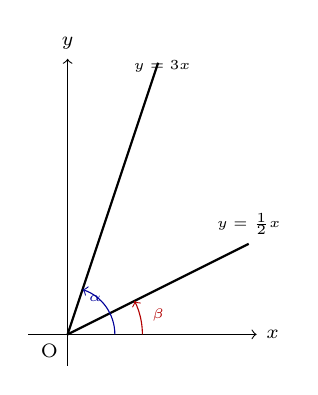
\begin{tikzpicture}[x=10mm,y=10mm]
\ax{-0.5}{2.4}{-0.4}{3.5}
\draw[thick,domain=0:1.15,samples=80] plot (\x,{3*\x});
\draw[thick,domain=0:2.3,samples=80] plot (\x,{0.5*\x});
\draw[->,blue!60!black] (0.6,0) arc (0:71.57:0.6); \draw[->,red!70!black] (0.95,0) arc (0:26.57:0.95); \node[blue!60!black] at (0.35,0.45){\tiny $\alpha$}; \node[red!70!black] at (1.15,0.25){\tiny $\beta$}; \node at (1.2,3.4){\tiny $y=3x$}; \node at (2.3,1.4){\tiny $y=\frac12x$};
\end{tikzpicture}
\end{center}
\hspace*{1.5em}$\tan(\alpha-\beta)=\dfrac{\tan\alpha-\tan\beta}{1+\tan\alpha\tan\beta}=\dfrac{3-\frac12}{1+3\cdot\frac12}=\dfrac{\frac52}{\frac52}=1$\\
\hspace*{1.5em}$0<\alpha-\beta<\dfrac\pi2$ だから\quad $\theta=\alpha-\beta=45^\circ$\quad $\left(\dfrac\pi4\right)$\\[2pt]
(2)\ 求める直線の傾きを $m$ とする．$y=2x$ とのなす角が $45^\circ$ だから\\
\hspace*{1.5em}$\left|\dfrac{m-2}{1+2m}\right|=\tan45^\circ=1$\quad （$1+2m\neq0$）\\
\hspace*{1.5em}$m-2=1+2m$ のとき $m=-3$．\quad $m-2=-(1+2m)$ のとき $3m=1$，$m=\dfrac13$．\\
\hspace*{1.5em}よって\quad $y=-3x$，\quad $y=\dfrac13x$\\
\hspace*{1.5em}（$y=2x$ を $\pm45^\circ$ 回転させた2本がある．）
\begin{center}
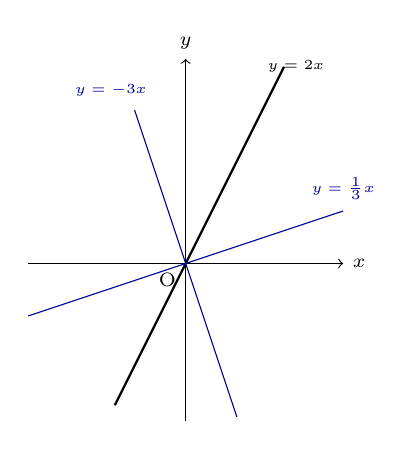
\begin{tikzpicture}[x=10mm,y=10mm]
\ax{-2}{2}{-2}{2.6}
\draw[thick,domain=-0.9:1.25,samples=80] plot (\x,{2*\x});
\draw[blue!60!black,domain=-0.65:0.65,samples=80] plot (\x,{-3*\x});
\draw[blue!60!black,domain=-2:2,samples=80] plot (\x,{\x/3});
\node at (1.4,2.5){\tiny $y=2x$}; \node[blue!60!black] at (-0.95,2.2){\tiny $y=-3x$}; \node[blue!60!black] at (2,0.95){\tiny $y=\frac13x$};
\end{tikzpicture}
\end{center}
\end{kai}

\ans{59}{三角関数の合成（Ⅰ）}
\begin{kai}
\textbf{方針}\quad \point{$a\sin\theta+b\cos\theta=\sqrt{a^2+b^2}\sin(\theta+\alpha)$}．$\alpha$ は\point{点 $(a,\ b)$ を座標平面にとったときの偏角}（$\cos\alpha=\dfrac a{\sqrt{a^2+b^2}}$，$\sin\alpha=\dfrac b{\sqrt{a^2+b^2}}$）．\\[2pt]
(1)\ $a=\sqrt3$，$b=1$．$r=\sqrt{3+1}=2$．\\
\begin{center}
\begin{tikzpicture}[x=12mm,y=12mm]
\ax{-0.5}{2.2}{-0.5}{1.5}
\fill (1.732,1) circle (1.6pt);
\node[above] at (1.732,1){\scriptsize $(\sqrt3,1)$};
\draw (0,0)--(1.732,1); \draw[->,blue!60!black] (0.6,0) arc (0:30:0.6); \node[blue!60!black] at (0.8,0.2){\tiny $\frac\pi6$}; \node at (0.7,0.65){\tiny 2};
\node[below] at (current bounding box.south){\scriptsize (1)};
\end{tikzpicture}\hspace{1.2em}
\begin{tikzpicture}[x=12mm,y=12mm]
\ax{-0.5}{1.6}{-1.5}{0.6}
\fill (1,-1) circle (1.6pt);
\node[right] at (1,-1){\scriptsize $(1,-1)$};
\draw (0,0)--(1,-1); \draw[->,blue!60!black] (0.5,0) arc (0:-45:0.5); \node[blue!60!black] at (0.75,-0.2){\tiny $-\frac\pi4$}; \node at (0.35,-0.65){\tiny $\sqrt2$};
\node[below] at (current bounding box.south){\scriptsize (2)};
\end{tikzpicture}
\end{center}
\hspace*{1.5em}$\cos\alpha=\dfrac{\sqrt3}2$，$\sin\alpha=\dfrac12$ より $\alpha=\dfrac\pi6$．\quad $\sqrt3\sin\theta+\cos\theta=2\sin\left(\theta+\dfrac\pi6\right)$\\[2pt]
(2)\ $a=1$，$b=-1$．$r=\sqrt{1+1}=\sqrt2$．\\
\hspace*{1.5em}$\cos\alpha=\dfrac1{\sqrt2}$，$\sin\alpha=-\dfrac1{\sqrt2}$ より $\alpha=-\dfrac\pi4$．\quad $\sin\theta-\cos\theta=\sqrt2\sin\left(\theta-\dfrac\pi4\right)$\\[2pt]
（検算：加法定理で展開すると，たとえば(1)は $2\left(\sin\theta\cdot\dfrac{\sqrt3}2+\cos\theta\cdot\dfrac12\right)$ でもとの式にもどる．）
\end{kai}

\ans{60}{三角関数の合成（Ⅱ）}
\begin{kai}
\textbf{方針}\quad 合成して $\sin$ 1つにまとめる．\point{$\theta+\alpha$ の範囲を求め}，単位円で $\sin$ のとる値の範囲を読む．\\[2pt]
$a=1$，$b=\sqrt3$ より $r=2$，$\alpha=\dfrac\pi3$．\quad $y=2\sin\left(\theta+\dfrac\pi3\right)$\\[2pt]
$0\leqq\theta\leqq\pi$ より\quad $\dfrac\pi3\leqq\theta+\dfrac\pi3\leqq\dfrac43\pi$\\
この範囲で $\sin\left(\theta+\dfrac\pi3\right)$ は，$\theta+\dfrac\pi3=\dfrac\pi2$ で最大値1，$\theta+\dfrac\pi3=\dfrac43\pi$ で最小値 $-\dfrac{\sqrt3}2$ をとる．\\
\begin{center}
\begin{tikzpicture}[scale=1,x=15mm,y=15mm]
\draw[->] (-1.35,0)--(1.4,0) node[right]{\tiny $x$}; \draw[->] (0,-1.35)--(0,1.4) node[above]{\tiny $y$}; \draw[gray] (0,0) circle (1); \node[below left] at (0,0){\tiny O};\draw[] (0.000,0.000)--(0.000,1.000);\fill (0.000,1.000) circle (1.4pt);\node[above right] at (0.000,1.000){\scriptsize 最大};\draw[] (0.000,0.000)--(-0.500,-0.866);\fill (-0.500,-0.866) circle (1.4pt);\node[below left] at (-0.500,-0.866){\scriptsize 最小};\draw[line width=2.5pt,blue!50] (60:1) arc (60:240:1); \fill (60:1) circle (1.4pt); \node[right] at (60:1){\tiny $\frac\pi3$}; \node[left] at (240:1.05){\tiny $\frac43\pi$};\node[below] at (current bounding box.south){\scriptsize $\theta+\frac\pi3$ の動く範囲（太線）};
\end{tikzpicture}
\end{center}
\hspace*{1.5em}（左端 $\dfrac\pi3$ での値は $\dfrac{\sqrt3}2$ で，右端の方が小さい．）\\[2pt]
最大値 $2\cdot1=2$\quad（$\theta+\dfrac\pi3=\dfrac\pi2$ より $\theta=\dfrac\pi6$）\\
最小値 $2\cdot\left(-\dfrac{\sqrt3}2\right)=-\sqrt3$\quad（$\theta+\dfrac\pi3=\dfrac43\pi$ より $\theta=\pi$）
\end{kai}

\ans{61}{三角関数の合成（Ⅲ）}
\begin{kai}
\textbf{方針}\quad $\sin^2\theta$，$\sin\theta\cos\theta$，$\cos^2\theta$ の2次式は，\point{2倍角・半角の公式で $2\theta$ の1次式に直してから合成}する．\\[2pt]
(1)\ \point{半角の公式で次数を下げる}\\
\hspace*{1.5em}$\sin^2\theta=\dfrac{1-\cos2\theta}2$，\quad $2\sin\theta\cos\theta=\sin2\theta$，\quad $\cos^2\theta=\dfrac{1+\cos2\theta}2$ を代入して\\
\hspace*{1.5em}$y=\dfrac{1-\cos2\theta}2+\sin2\theta+\dfrac{3(1+\cos2\theta)}2=\sin2\theta+\dfrac{-1+3}2\cos2\theta+\dfrac{1+3}2$\\
\hspace*{1.5em}$=\sin2\theta+\cos2\theta+2$\\[2pt]
(2)\ $\sin2\theta+\cos2\theta=\sqrt2\sin\left(2\theta+\dfrac\pi4\right)$ と合成して\quad $y=\sqrt2\sin\left(2\theta+\dfrac\pi4\right)+2$\\
\hspace*{1.5em}$0\leqq\theta\leqq\dfrac\pi2$ より $\dfrac\pi4\leqq2\theta+\dfrac\pi4\leqq\dfrac54\pi$．この範囲で\quad $-\dfrac{\sqrt2}2\leqq\sin\left(2\theta+\dfrac\pi4\right)\leqq1$\\[2pt]
\begin{center}
\begin{tikzpicture}[scale=1,x=15mm,y=15mm]
\draw[->] (-1.35,0)--(1.4,0) node[right]{\tiny $x$}; \draw[->] (0,-1.35)--(0,1.4) node[above]{\tiny $y$}; \draw[gray] (0,0) circle (1); \node[below left] at (0,0){\tiny O};\draw[] (0.000,0.000)--(0.000,1.000);\fill (0.000,1.000) circle (1.4pt);\node[above right] at (0.000,1.000){\scriptsize 最大};\draw[] (0.000,0.000)--(-0.707,-0.707);\fill (-0.707,-0.707) circle (1.4pt);\node[below left] at (-0.707,-0.707){\scriptsize 最小};\draw[line width=2.5pt,blue!50] (45:1) arc (45:225:1); \node[right] at (45:1){\tiny $\frac\pi4$}; \node[left] at (225:1.05){\tiny $\frac54\pi$};\node[below] at (current bounding box.south){\scriptsize $2\theta+\frac\pi4$ の動く範囲（太線）};
\end{tikzpicture}
\end{center}
\hspace*{1.5em}最大値：$2\theta+\dfrac\pi4=\dfrac\pi2$，すなわち $\theta=\dfrac\pi8$ のとき\quad $\sqrt2+2$\\
\hspace*{1.5em}最小値：$2\theta+\dfrac\pi4=\dfrac54\pi$，すなわち $\theta=\dfrac\pi2$ のとき\quad $\sqrt2\cdot\left(-\dfrac{\sqrt2}2\right)+2=1$
\end{kai}

\ans{62}{三角関数のグラフ}
\begin{kai}
\textbf{方針}\quad $y=a\sin(k\theta-b)$ は，\point{$y=a\sin k(\theta-\tfrac bk)$ と $k$ でくくる}と平行移動の量がわかる．周期は $\dfrac{2\pi}{k}$．\\[2pt]
(1)\ $y=2\sin2\left(\theta-\dfrac\pi6\right)$．$\sin$ の周期は $2\pi$ なので，$2\theta$ の係数2で割って周期は\quad $\dfrac{2\pi}2=\pi$\\
\hspace*{1.5em}$-1\leqq\sin\left(2\theta-\dfrac\pi3\right)\leqq1$ より\quad 最大値 $2$，\quad 最小値 $-2$\\[2pt]
(2)\ \point{$2\theta-\dfrac\pi3=2\left(\theta-\dfrac\pi6\right)$ と $\theta$ の係数でくくる}\\
\hspace*{1.5em}$y=2\sin2\left(\theta-\dfrac\pi6\right)$ は，$y=2\sin2\theta$ の $\theta$ を $\theta-\dfrac\pi6$ におきかえたもの．\\
\hspace*{1.5em}よって，$\theta$ 軸方向に $\dfrac\pi6$ だけ平行移動したもの\\
\hspace*{1.5em}\point{$\dfrac\pi3$ だけ移動ではない}\\[2pt]
\begin{center}
\begin{tikzpicture}[x=10mm,y=7mm]
\ax{-0.7}{3.6}{-2.6}{2.8}
\draw[dashed,gray,domain=-0.5:3.3,samples=80] plot (\x,{2*sin(2*\x r)});
\draw[thick,domain=-0.5:3.3,samples=80] plot (\x,{2*sin((2*\x-pi/3) r)});
\draw (0.5236,0.12)--(0.5236,-0.12); \node[below] at (0.5236,0){\tiny $\frac\pi6$};
\draw (1.5708,0.12)--(1.5708,-0.12); \node[below] at (1.5708,0){\tiny $\frac\pi2$};
\draw (2.0944,0.12)--(2.0944,-0.12); \node[below] at (2.0944,0){\tiny $\frac23\pi$};
\draw (3.1416,0.12)--(3.1416,-0.12); \node[below] at (3.1416,0){\tiny $\pi$};
\node[left] at (0,2){\tiny $2$};
\node[left] at (0,-2){\tiny $-2$};
\draw[->,blue!60!black] (0.785,2.15)--(1.309,2.15); \node[blue!60!black] at (1.05,2.5){\tiny $\frac\pi6$};
\node[below] at (current bounding box.south){\scriptsize 点線：$y=2\sin2\theta$，実線：$y=2\sin\left(2\theta-\frac\pi3\right)$};
\end{tikzpicture}
\end{center}
(3)\ $0\leqq\theta<\pi$ より\quad $-\dfrac\pi3\leqq2\theta-\dfrac\pi3<\dfrac53\pi$\\
\hspace*{1.5em}この範囲で $\sin\left(2\theta-\dfrac\pi3\right)=0$ となるのは\quad $2\theta-\dfrac\pi3=0,\ \pi$\\
\hspace*{1.5em}よって\quad $\theta=\dfrac\pi6,\ \dfrac23\pi$
\end{kai}

\ans{63}{三角方程式}
\begin{kai}
\textbf{方針}\quad (1)は $\cos^2\theta=1-\sin^2\theta$ で\point{$\sin\theta$ に統一}．(2)は\point{移項して合成}し，$\theta-\dfrac\pi4$ の範囲で考える．\\[2pt]
(1)\ $2(1-\sin^2\theta)+3\sin\theta-3=0$，\quad $-2\sin^2\theta+3\sin\theta-1=0$\\
\hspace*{1.5em}$2\sin^2\theta-3\sin\theta+1=0$，\quad $(2\sin\theta-1)(\sin\theta-1)=0$\\
\hspace*{1.5em}$\sin\theta=\dfrac12$ のとき\quad $\theta=\dfrac\pi6,\ \dfrac56\pi$\\
\hspace*{1.5em}$\sin\theta=1$ のとき\quad $\theta=\dfrac\pi2$\\
\hspace*{1.5em}よって\quad $\theta=\dfrac\pi6,\ \dfrac\pi2,\ \dfrac56\pi$\\[2pt]
\begin{center}
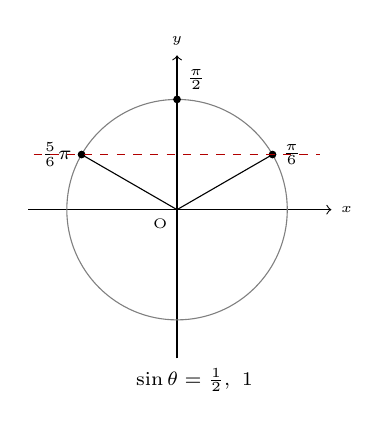
\begin{tikzpicture}[scale=1,x=14mm,y=14mm]
\draw[->] (-1.35,0)--(1.4,0) node[right]{\tiny $x$}; \draw[->] (0,-1.35)--(0,1.4) node[above]{\tiny $y$}; \draw[gray] (0,0) circle (1); \node[below left] at (0,0){\tiny O};\draw[] (0.000,0.000)--(0.866,0.500);\fill (0.866,0.500) circle (1.4pt);\node[right] at (0.866,0.500){\scriptsize $\frac\pi6$};\draw[] (0.000,0.000)--(-0.866,0.500);\fill (-0.866,0.500) circle (1.4pt);\node[left] at (-0.866,0.500){\scriptsize $\frac56\pi$};\draw[] (0.000,0.000)--(0.000,1.000);\fill (0.000,1.000) circle (1.4pt);\node[above right] at (0.000,1.000){\scriptsize $\frac\pi2$};\draw[dashed,red!70!black] (-1.3,0.5)--(1.3,0.5);\node[below] at (current bounding box.south){\scriptsize $\sin\theta=\frac12,\ 1$};
\end{tikzpicture}
\end{center}
(2)\ $\sin\theta-\cos\theta>0$．合成して\quad $\sqrt2\sin\left(\theta-\dfrac\pi4\right)>0$\\
\hspace*{1.5em}$0\leqq\theta<2\pi$ より $-\dfrac\pi4\leqq\theta-\dfrac\pi4<\dfrac74\pi$．この範囲で $\sin>0$ となるのは\quad $0<\theta-\dfrac\pi4<\pi$\\
\hspace*{1.5em}よって\quad $\dfrac\pi4<\theta<\dfrac54\pi$\\
\hspace*{1.5em}（単位円で，直線 $y=x$ より上側にある部分と考えてもよい．）
\begin{center}
\begin{tikzpicture}[scale=1,x=14mm,y=14mm]
\draw[->] (-1.35,0)--(1.4,0) node[right]{\tiny $x$}; \draw[->] (0,-1.35)--(0,1.4) node[above]{\tiny $y$}; \draw[gray] (0,0) circle (1); \node[below left] at (0,0){\tiny O};\draw[] (0.000,0.000)--(0.707,0.707);\fill (0.707,0.707) circle (1.4pt);\node[right] at (0.707,0.707){\scriptsize $\frac\pi4$};\draw[] (0.000,0.000)--(-0.707,-0.707);\fill (-0.707,-0.707) circle (1.4pt);\node[left] at (-0.707,-0.707){\scriptsize $\frac54\pi$};\draw[line width=2.5pt,blue!50] (45:1) arc (45:225:1); \draw[dashed,red!70!black] (-1.2,-1.2)--(1.2,1.2);\node[below] at (current bounding box.south){\scriptsize $\sin\theta>\cos\theta$ の部分（太線）};
\end{tikzpicture}
\end{center}
\end{kai}

\shouans{第5章}{指数関数と対数関数}
\ans{64}{指数の計算}
\begin{kai}
\textbf{方針}\quad 累乗根は\point{分数の指数に直し}，底を素数にそろえて指数法則 $a^pa^q=a^{p+q}$，$(a^p)^q=a^{pq}$ を使う．(3)は対称式と同じ変形．\\[2pt]
(1)\ (i)\ $8^{\frac23}=(2^3)^{\frac23}=2^2=4$\\
\hspace*{1.5em}(ii)\ $27^{-\frac13}=(3^3)^{-\frac13}=3^{-1}=\dfrac13$\\
\hspace*{1.5em}(iii)\ $\sqrt[3]4\times\sqrt[3]{16}=\sqrt[3]{64}=\sqrt[3]{4^3}=4$\\[2pt]
(2)\ $\sqrt a=a^{\frac12}$，$\sqrt[4]{a^3}=a^{\frac34}$，$\sqrt[4]a=a^{\frac14}$ だから\\
\hspace*{1.5em}$a^{\frac12}\times a^{\frac34}\div a^{\frac14}=a^{\frac12+\frac34-\frac14}=a^1=a$\\[2pt]
(3)\ \point{2乗・3乗して整理}．$x^{\frac12}\cdot x^{-\frac12}=1$ に注意する．\\
\hspace*{1.5em}$\left(x^{\frac12}+x^{-\frac12}\right)^2=x+2+x^{-1}$ より\quad $x+x^{-1}=3^2-2=7$\\[2pt]
\hspace*{1.5em}$\left(x^{\frac12}+x^{-\frac12}\right)^3=x^{\frac32}+3x^{\frac12}+3x^{-\frac12}+x^{-\frac32}$ より\\
\hspace*{1.5em}$x^{\frac32}+x^{-\frac32}=\left(x^{\frac12}+x^{-\frac12}\right)^3-3\left(x^{\frac12}+x^{-\frac12}\right)=27-9=18$
\end{kai}

\ans{65}{指数関数のグラフ}
\begin{kai}
\textbf{方針}\quad (1)は\point{$x$ を $x-p$，$y$ を $y-q$ におきかえると平行移動}．(2)は\point{底を2にそろえて指数を比べる}（底 $>1$ なら指数が大きいほど大きい）．\\[2pt]
(1)\ $y-3=2^{x-1}$ と変形すると，$y=2^x$ の $x$ を $x-1$，$y$ を $y-3$ におきかえた形．\\
\hspace*{1.5em}よって\quad $x$ 軸方向に1，$y$ 軸方向に3だけ平行移動したもの\\
\hspace*{1.5em}$y=2^x$ の漸近線は $x$ 軸（$y=0$）なので，移動後の漸近線は\quad 直線 $y=3$\\[2pt]
(2)\ \point{底を2にそろえる}\\
\hspace*{1.5em}$\sqrt[3]2=2^{\frac13}$，\quad $\sqrt[4]4=4^{\frac14}=2^{\frac24}=2^{\frac12}$，\quad $\sqrt[5]8=8^{\frac15}=2^{\frac35}$\\
\hspace*{1.5em}指数を通分して比べると\quad $\dfrac13=\dfrac{10}{30}$，$\dfrac12=\dfrac{15}{30}$，$\dfrac35=\dfrac{18}{30}$\\
\hspace*{1.5em}底 $2>1$ だから，指数の大小と数の大小が一致する．\quad $\sqrt[3]2<\sqrt[4]4<\sqrt[5]8$
\end{kai}

\ans{66}{指数方程式（Ⅰ）}
\begin{kai}
\textbf{方針}\quad \point{両辺の底をそろえて，指数を比較する}（$a^p=a^q\iff p=q$）．\\[2pt]
(1)\ $8=2^3$ だから $8^{x-1}=(2^3)^{x-1}=2^{3x-3}$．\\
\hspace*{1.5em}$2^{x+1}=2^{3x-3}$ より $x+1=3x-3$，\quad $2x=4$，\quad $x=2$\\[2pt]
(2)\ $9=3^2$，$\dfrac1{27}=3^{-3}$ だから\quad $3^{2x}=3^{-3}$\\
\hspace*{1.5em}$2x=-3$ より\quad $x=-\dfrac32$
\end{kai}

\ans{67}{指数方程式（Ⅱ）}
\begin{kai}
\textbf{方針}\quad $4^x=(2^x)^2$ に注目して\point{$2^x=t$ とおき，$t$ の2次方程式にする}．\point{$t>0$} なので負の解は除く．\\[2pt]
(1)\ $4^x=(2^2)^x=(2^x)^2$．$t=2^x$（$t>0$）とおくと\\
\hspace*{1.5em}$t^2-3t-4=0$，\quad $(t-4)(t+1)=0$．$t>0$ より $t=4$．\\
\hspace*{1.5em}$2^x=4=2^2$ より\quad $x=2$\\[2pt]
(2)\ $9^x=(3^x)^2$，$3^{x+1}=3\cdot3^x$．$t=3^x$（$t>0$）とおくと\\
\hspace*{1.5em}$t^2+3t-18=0$，\quad $(t+6)(t-3)=0$．$t>0$ より $t=3$．\\
\hspace*{1.5em}$3^x=3$ より\quad $x=1$
\end{kai}

\ans{68}{指数不等式}
\begin{kai}
\textbf{方針}\quad 底をそろえて指数を比べる．\point{底 $>1$ なら不等号の向きはそのまま，$0<$ 底 $<1$ なら逆}．(2)は $2^x=t$ とおく．\\[2pt]
(1)\ $\left(\dfrac12\right)^x=2^{-x}$，$8=2^3$ だから\quad $2^{-x}>2^3$\\
\hspace*{1.5em}底 $2>1$ だから $-x>3$，\quad $x<-3$\\
\hspace*{1.5em}（底を $\dfrac12$ にそろえると $\left(\dfrac12\right)^x>\left(\dfrac12\right)^{-3}$，底 $<1$ なので $x<-3$ となり同じ．）\\[2pt]
(2)\ $t=2^x$（$t>0$）とおくと\quad $t^2-6t+8<0$，\quad $(t-2)(t-4)<0$，\quad $2<t<4$\\
\hspace*{1.5em}（これは $t>0$ をみたす．）\quad $2^1<2^x<2^2$．底 $2>1$ だから\quad $1<x<2$
\end{kai}

\ans{69}{対数の計算（Ⅰ）}
\begin{kai}
\textbf{方針}\quad 対数の性質 \point{$\log_aM+\log_aN=\log_aMN$，$\log_aM-\log_aN=\log_a\dfrac MN$，$k\log_aM=\log_aM^k$} で1つの対数にまとめる．\\[2pt]
(1)\ $\log_248-\log_23=\log_2\dfrac{48}3=\log_216=\log_22^4=4$\\[2pt]
(2)\ $\sqrt{27}=(3^3)^{\frac12}=3^{\frac32}$ だから\quad $\log_3\sqrt{27}=\log_33^{\frac32}=\dfrac32$\\[2pt]
(3)\ $2\log_{10}5=\log_{10}5^2=\log_{10}25$ だから\\
\hspace*{1.5em}$2\log_{10}5+\log_{10}4=\log_{10}(25\times4)=\log_{10}100=2$
\end{kai}

\ans{70}{対数の計算（Ⅱ）}
\begin{kai}
\textbf{方針}\quad 底がそろっていないときは\point{底の変換公式 $\log_ab=\dfrac{\log_cb}{\log_ca}$} で底をそろえる．\point{$a^{\log_aM}=M$}．\\[2pt]
(1)\ 底を2にそろえて\quad $\log_48=\dfrac{\log_28}{\log_24}=\dfrac{3}{2}$\\
\hspace*{1.5em}（確認：$4^{\frac32}=(2^2)^{\frac32}=2^3=8$）\\[2pt]
(2)\ $\log_29=\log_23^2=2\log_23$，\quad $\log_38=3\log_32=3\cdot\dfrac{\log_22}{\log_23}=\dfrac3{\log_23}$\\
\hspace*{1.5em}よって\quad $\log_29\cdot\log_38=2\log_23\cdot\dfrac3{\log_23}=6$\\[2pt]
(3)\ $\log_35=p$ とおくと，対数の定義より $3^p=5$．よって\quad $3^{\log_35}=5$
\end{kai}

\ans{71}{対数関数のグラフ}
\begin{kai}
\textbf{方針}\quad (1)は $x\to x-p$，$y\to y-q$ で平行移動．(2)は\point{底を2にそろえて真数を比べる}（底 $>1$ なら真数が大きいほど大きい）．\\[2pt]
(1)\ $y-2=\log_2(x-1)$ と変形すると，$y=\log_2x$ の $x$ を $x-1$，$y$ を $y-2$ におきかえた形．\\
\hspace*{1.5em}$x$ 軸方向に1，$y$ 軸方向に2だけ平行移動したもの\\
\hspace*{1.5em}（$y=\log_2x$ の漸近線は $y$ 軸なので，移動後の漸近線は直線 $x=1$）\\[2pt]
(2)\ 底を2にそろえる．\\
\hspace*{1.5em}$2=2\log_22=\log_24$，\quad $\log_430=\dfrac{\log_230}{\log_24}=\dfrac{\log_230}{2}=\log_230^{\frac12}=\log_2\sqrt{30}$\\
\hspace*{1.5em}真数を比べると $4<5<\sqrt{30}$（$\sqrt{25}<\sqrt{30}$）．底 $2>1$ だから\\
\hspace*{1.5em}$2<\log_25<\log_430$
\end{kai}

\ans{72}{対数方程式（Ⅰ）}
\begin{kai}
\textbf{方針}\quad \point{まず真数条件（真数 $>0$）}を確認する．対数を1つにまとめ，$\log_aM=\log_aN\iff M=N$ を使う．\\[2pt]
真数条件：$x+1>0$ かつ $x-1>0$ より\quad $x>1$\\[2pt]
左辺をまとめて $\log_2(x+1)(x-1)=3$．$3=\log_28$ だから\\
\hspace*{1.5em}$\log_2(x^2-1)=\log_28$，\quad $x^2-1=8$，\quad $x^2=9$，\quad $x=\pm3$\\
$x>1$ より\quad $x=3$\\
\point{$x=-3$ は $x^2-1=8$ をみたすが，もとの式の真数が負になるので不適}
\end{kai}

\ans{73}{対数方程式（Ⅱ）}
\begin{kai}
\textbf{方針}\quad $\log_2x^3=3\log_2x$ と変形し，\point{$\log_2x=t$ とおいて $t$ の2次方程式}にする．$t$ はすべての実数をとる．\\[2pt]
真数条件：$x>0$（$x^3>0$ も同じ条件）\\
$\log_2x^3=3\log_2x$ だから，$t=\log_2x$ とおくと\\
\hspace*{1.5em}$t^2-3t+2=0$，\quad $(t-1)(t-2)=0$，\quad $t=1,\ 2$\\
$\log_2x=1$ より $x=2$，\quad $\log_2x=2$ より $x=4$．どちらも $x>0$ をみたす．\\[2pt]
よって\quad $x=2,\ 4$\\
\point{$(\log_2x)^2$ と $\log_2x^2$ は別物．$(\log_2x)^2\neq2\log_2x$}
\end{kai}

\ans{74}{対数不等式}
\begin{kai}
\textbf{方針}\quad 真数条件を確認し，右辺も同じ底の対数にして真数を比べる．\point{底が1より小さいと不等号の向きが逆}．最後に真数条件との共通部分をとる．\\[2pt]
(1)\ 真数条件：$x-1>0$ より $x>1$．\\
\hspace*{1.5em}$-2=-2\log_{\frac12}\dfrac12=\log_{\frac12}\left(\dfrac12\right)^{-2}=\log_{\frac12}4$ だから\quad $\log_{\frac12}(x-1)>\log_{\frac12}4$\\
\hspace*{1.5em}底 $\dfrac12<1$ だから，真数の大小は逆になり\quad $x-1<4$，\quad $x<5$\\
\hspace*{1.5em}真数条件と合わせて\quad $1<x<5$\\[2pt]
(2)\ 真数条件：$x>0$ かつ $x-2>0$ より $x>2$．\\
\hspace*{1.5em}$\log_2x(x-2)\leqq\log_28$．底 $2>1$ だから\quad $x(x-2)\leqq8$\\
\hspace*{1.5em}$x^2-2x-8\leqq0$，\quad $(x+2)(x-4)\leqq0$，\quad $-2\leqq x\leqq4$\\
\hspace*{1.5em}真数条件と合わせて\quad $2<x\leqq4$
\end{kai}

\ans{75}{対数の応用（Ⅰ）}
\begin{kai}
\textbf{方針}\quad \point{$N$ の常用対数が $n\leqq\log_{10}N<n+1$ なら $N$ は $n+1$ 桁}．最高位の数字は，\point{小数部分 $\log_{10}N-n$ が $\log_{10}k$ と $\log_{10}(k+1)$ の間にあれば $k$}．\\[2pt]
(1)\ $\log_{10}2^{50}=50\log_{10}2=50\times0.3010=15.05$\\
\hspace*{1.5em}$15<15.05<16$ より $10^{15}<2^{50}<10^{16}$．\\
\hspace*{1.5em}$10^{15}$ は16桁の最小の数なので，$2^{50}$ は\quad 16桁\\[2pt]
(2)\ $2^{50}=10^{15.05}=10^{0.05}\times10^{15}$．最高位の数字は $10^{0.05}$ の整数部分．\\
\hspace*{1.5em}$\log_{10}1=0<0.05<0.3010=\log_{10}2$ より\quad $1<10^{0.05}<2$\\
\hspace*{1.5em}よって $2^{50}=1.\cdots\times10^{15}$ となり，最高位の数字は\quad 1
\end{kai}

\ans{76}{対数の応用（Ⅱ）}
\begin{kai}
\textbf{方針}\quad \point{両辺の常用対数をとる}（底 $10>1$ なので不等号の向きは変わらない）．$\log_{10}\dfrac13=-\log_{10}3$．負の数で割ると向きが変わることに注意．\\[2pt]
$\left(\dfrac13\right)^n<10^{-10}$ の両辺の常用対数をとって\\
\hspace*{1.5em}$\log_{10}\left(\dfrac13\right)^n<\log_{10}10^{-10}$，\quad $-n\log_{10}3<-10$\\
両辺を $-\log_{10}3\ (<0)$ で割ると向きが変わり\\
\hspace*{1.5em}$n>\dfrac{10}{\log_{10}3}=\dfrac{10}{0.4771}=20.9\cdots$\\
これをみたす最小の自然数は\quad $n=21$
\end{kai}

\ans{77}{指数・対数関数の最大・最小}
\begin{kai}
\textbf{方針}\quad \point{おきかえて2次関数にする}．(1)は $t=2^x$，(2)は $t=\log_2x$．\point{$x$ の範囲から $t$ の範囲を求める}ことを忘れない．\\[2pt]
(1)\ $4^x=(2^x)^2$，$2^{x+2}=4\cdot2^x$．$t=2^x$ とおくと，$0\leqq x\leqq2$ より $2^0\leqq t\leqq2^2$，すなわち\quad $1\leqq t\leqq4$\\
\hspace*{1.5em}$y=t^2-4t+5=(t-2)^2+1$\\
\hspace*{1.5em}$1\leqq t\leqq4$ で，$t=2$ のとき最小，軸から遠い $t=4$ のとき最大（$t=1$ のとき $y=2$）．\\
\hspace*{1.5em}最大値 $5$（$t=4$ より $x=2$），\quad 最小値 $1$（$t=2$ より $x=1$）\\[2pt]
(2)\ $\log_2x^2=2\log_2x$．$t=\log_2x$ とおくと，$1\leqq x\leqq8$ より $\log_21\leqq t\leqq\log_28$，すなわち\quad $0\leqq t\leqq3$\\
\hspace*{1.5em}$y=t^2-2t=(t-1)^2-1$\\
\hspace*{1.5em}$0\leqq t\leqq3$ で，$t=1$ のとき最小，$t=3$ のとき最大（$t=0$ のとき $y=0$）．\\
\hspace*{1.5em}最大値 $3$（$t=3$ より $x=8$），\quad 最小値 $-1$（$t=1$ より $x=2$）
\end{kai}

\ans{78}{大小比較（Ⅰ）}
\begin{kai}
\textbf{方針}\quad 累乗根の指数 2，3，6 の\point{最小公倍数の6乗}をすると，すべて整数になって比べやすい．正の数どうしなら，6乗しても大小は変わらない．\\[2pt]
\point{6乗して比べる}\\
\hspace*{1.5em}$(\sqrt2)^6=(2^{\frac12})^6=2^3=8$\\
\hspace*{1.5em}$(\sqrt[3]3)^6=(3^{\frac13})^6=3^2=9$\\
\hspace*{1.5em}$(\sqrt[6]6)^6=6$\\
$6<8<9$ で，3数はすべて正だから\quad $\sqrt[6]6<\sqrt2<\sqrt[3]3$
\end{kai}

\ans{79}{大小比較（Ⅱ）}
\begin{kai}
\textbf{方針}\quad 底の違う対数は直接比べにくいので，\point{間に $\dfrac32$ をはさんで，それぞれと $\dfrac32$ を比べる}．$\dfrac32$ を同じ底の対数で表す．\\[2pt]
$\dfrac32=\dfrac12\log_28=\log_2\sqrt8$，\quad $\dfrac32=\dfrac12\log_327=\log_3\sqrt{27}$ と表せる．\\[2pt]
$\log_23-\dfrac32=\log_23-\dfrac12\log_28=\dfrac12(2\log_23-\log_28)=\dfrac12(\log_29-\log_28)>0$\\
\hspace*{1.5em}（底 $2>1$ で $9>8$）．よって\quad $\log_23>\dfrac32$\\[2pt]
$\log_34-\dfrac32=\dfrac12(\log_316-\log_327)<0$\\
\hspace*{1.5em}（底 $3>1$ で $16<27$）．よって\quad $\log_34<\dfrac32$\\[2pt]
したがって\quad $\log_34<\dfrac32<\log_23$
\end{kai}

\ans{80}{常用対数の値の評価}
\begin{kai}
\textbf{方針}\quad 与えられた大小関係（$2^{10}>10^3$，$2^3<10$）の\point{両辺の常用対数をとる}．底 $10>1$ なので不等号の向きは変わらない．\\[2pt]
$2^{10}=1024>1000=10^3$ の両辺の常用対数をとって\\
\hspace*{1.5em}$\log_{10}2^{10}>\log_{10}10^3$，\quad $10\log_{10}2>3$，\quad $\log_{10}2>0.3$\\[2pt]
$2^3=8<10$ の両辺の常用対数をとって\\
\hspace*{1.5em}$\log_{10}2^3<\log_{10}10$，\quad $3\log_{10}2<1$，\quad $\log_{10}2<\dfrac13$\\[2pt]
よって\quad $0.3<\log_{10}2<\dfrac13$\\
（実際の値 $\log_{10}2=0.3010\cdots$ はこの範囲にある．）
\end{kai}

\shouans{第6章}{微分法と積分法}
\ans{81}{極限（Ⅰ）}
\begin{kai}
\textbf{方針}\quad そのまま代入すると $\dfrac00$ になる．\point{分母・分子を因数分解して，0になる因数を約分してから代入}する．\\[2pt]
(1)\ $x\neq2$ では $\dfrac{x^2-4}{x-2}=\dfrac{(x+2)(x-2)}{x-2}=x+2$ だから\\
\hspace*{1.5em}$\displaystyle\lim_{x\to2}\frac{x^2-4}{x-2}=\lim_{x\to2}(x+2)=4$\\[2pt]
(2)\ $x^3-1=(x-1)(x^2+x+1)$，$x^2-1=(x-1)(x+1)$ だから\\
\hspace*{1.5em}$\displaystyle\lim_{x\to1}\frac{x^3-1}{x^2-1}=\lim_{x\to1}\frac{(x-1)(x^2+x+1)}{(x-1)(x+1)}=\lim_{x\to1}\frac{x^2+x+1}{x+1}=\frac32$\\
\point{$x\to1$ では $x\neq1$ なので，$x-1$ で約分してよい}
\end{kai}

\ans{82}{極限（Ⅱ）}
\begin{kai}
\textbf{方針}\quad \point{分母 $\to0$ のとき極限値が存在するなら，分子 $\to0$}（必要条件）．これで $a,\ b$ の関係を出し，約分して極限値を計算する．\\[2pt]
$\displaystyle\lim_{x\to1}(x-1)=0$ だから，極限値が存在するためには\quad $\displaystyle\lim_{x\to1}(x^2+ax+b)=1+a+b=0$\\
\hspace*{1.5em}（もし分子 $\to c\neq0$ なら，$\dfrac{c}{0}$ の形で発散してしまう．）\\
よって\quad $b=-a-1$\\[2pt]
このとき分子は\quad $x^2+ax-a-1=(x^2-1)+a(x-1)=(x-1)(x+1+a)$\\
\hspace*{1.5em}$\displaystyle\lim_{x\to1}\frac{(x-1)(x+a+1)}{x-1}=\lim_{x\to1}(x+a+1)=a+2$\\
これが3に等しいので\quad $a+2=3$，\quad $a=1$，\quad $b=-2$\\
（確認：$\dfrac{x^2+x-2}{x-1}=\dfrac{(x-1)(x+2)}{x-1}=x+2\to3$）
\end{kai}

\ans{83}{導関数}
\begin{kai}
\textbf{方針}\quad 導関数の定義 \point{$f'(x)=\displaystyle\lim_{h\to0}\frac{f(x+h)-f(x)}{h}$}．計算では $(x^n)'=nx^{n-1}$ を使い，積の形は\point{展開してから}微分する．\\[2pt]
(1)\ $(x+h)^3-x^3=x^3+3x^2h+3xh^2+h^3-x^3=3x^2h+3xh^2+h^3$ だから\\
\hspace*{1.5em}$f'(x)=\displaystyle\lim_{h\to0}\frac{3x^2h+3xh^2+h^3}{h}=\lim_{h\to0}(3x^2+3xh+h^2)=3x^2$\\[2pt]
(2)\ 展開して\quad $y=2x^3+6x-x^2-3=2x^3-x^2+6x-3$\\
\hspace*{1.5em}$y'=2\cdot3x^2-2x+6=6x^2-2x+6$
\end{kai}

\ans{84}{微分係数}
\begin{kai}
\textbf{方針}\quad \point{$f'(a)=\displaystyle\lim_{h\to0}\frac{f(a+h)-f(a)}{h}$}．分子を展開して $h$ でくくり，約分してから $h\to0$ とする．\\[2pt]
$f(2)=8-4=4$\\
$f(2+h)=(2+h)^3-2(2+h)=8+12h+6h^2+h^3-4-2h=4+10h+6h^2+h^3$\\
よって\quad $f(2+h)-f(2)=10h+6h^2+h^3$\\[2pt]
$f'(2)=\displaystyle\lim_{h\to0}\frac{10h+6h^2+h^3}{h}=\lim_{h\to0}(10+6h+h^2)=10$\\
（検算：$f'(x)=3x^2-2$ より $f'(2)=12-2=10$）
\end{kai}

\ans{85}{平均変化率と微分係数}
\begin{kai}
\textbf{方針}\quad \point{平均変化率は $\dfrac{f(b)-f(a)}{b-a}$}（2点を結ぶ直線の傾き），その $h\to0$ の極限が微分係数（接線の傾き）．\\[2pt]
(1)\ $f(1)=2$，\quad $f(1+h)=(1+h)^2+(1+h)=2+3h+h^2$\\
\hspace*{1.5em}平均変化率は\quad $\dfrac{f(1+h)-f(1)}{(1+h)-1}=\dfrac{3h+h^2}{h}=3+h$\\
\hspace*{1.5em}$f'(1)=\displaystyle\lim_{h\to0}(3+h)=3$\\[2pt]
(2)\ $f(0)=0$，$f(2)=6$ だから，平均変化率は\quad $\dfrac{6-0}{2-0}=3$\\
\hspace*{1.5em}$f'(x)=2x+1$ だから，$f'(c)=2c+1=3$ より\quad $c=1$\\
\hspace*{1.5em}（2点 $(0,\ 0)$，$(2,\ 6)$ を結ぶ直線と平行な接線の接点が $x=1$．$0<c<2$ をみたす．）
\end{kai}

\ans{86}{接線（Ⅰ）}
\begin{kai}
\textbf{方針}\quad \point{曲線 $y=f(x)$ 上の点 $(a,\ f(a))$ における接線は $y-f(a)=f'(a)(x-a)$}．法線は接線に垂直なので傾きは $-\dfrac{1}{f'(a)}$．\\[2pt]
$y'=3x^2-3$．$x=2$ のとき $y'=12-3=9$．\\[2pt]
接線：傾き9で点 $(2,\ 2)$ を通るので\quad $y-2=9(x-2)$，\quad $y=9x-16$\\[2pt]
法線：傾きは $-\dfrac19$（傾きの積が $-1$）．\quad $y-2=-\dfrac19(x-2)$，\quad $y=-\dfrac19x+\dfrac{20}9$
\end{kai}

\ans{87}{接線（Ⅱ）}
\begin{kai}
\textbf{方針}\quad 曲線外の点からの接線は，\point{接点を $(t,\ f(t))$ とおいて接線の式をつくり，それが与えられた点を通る条件}から $t$ を求める．\\[2pt]
$y'=2x$．接点を $(t,\ t^2)$ とすると，接線は\\
\hspace*{1.5em}$y-t^2=2t(x-t)$，\quad $y=2tx-t^2$ ……①\\
①が点 $(1,\ -3)$ を通るので\quad $-3=2t-t^2$，\quad $t^2-2t-3=0$，\quad $(t-3)(t+1)=0$\\
\hspace*{1.5em}$t=3$ のとき①は\quad $y=6x-9$\quad （接点 $(3,\ 9)$）\\
\hspace*{1.5em}$t=-1$ のとき①は\quad $y=-2x-1$\quad （接点 $(-1,\ 1)$）\\
\point{点 $(1,\ -3)$ は曲線上にないので，$y'$ に $x=1$ を代入して傾きとしてはいけない}
\end{kai}

\ans{88}{関数決定（Ⅰ）}
\begin{kai}
\textbf{方針}\quad $f'(x)$ を求め，与えられた3つの条件を\point{$a,\ b,\ c$ の連立方程式}にする．\\[2pt]
$f'(x)=2ax+b$\\
$f'(0)=-3$ より\quad $b=-3$\\
$f'(1)=1$ より\quad $2a+b=1$，\quad $2a=4$，\quad $a=2$\\
$f(1)=2$ より\quad $a+b+c=2$，\quad $2-3+c=2$，\quad $c=3$\\[2pt]
よって\quad $f(x)=2x^2-3x+3$
\end{kai}

\ans{89}{3次関数のグラフ}
\begin{kai}
\textbf{方針}\quad $y'$ を因数分解して $y'=0$ となる $x$ を求め，\point{増減表}をつくる．$y'$ の符号が $+$ から $-$ に変わる点で極大，$-$ から $+$ で極小．\\[2pt]
\begin{minipage}[t]{0.58\linewidth}
$y'=3x^2-6x-9=3(x+1)(x-3)$\\[2pt]
\renewcommand{\arraystretch}{1.1}
$\begin{array}{c|ccccc}
x&\cdots&-1&\cdots&3&\cdots\\ \hline
y'&+&0&-&0&+\\ \hline
y&\nearrow&10&\searrow&-22&\nearrow
\end{array}$\\[4pt]
$y(-1)=-1-3+9+5=10$，\quad $y(3)=27-27-27+5=-22$\\
極大値 $10$（$x=-1$），\quad 極小値 $-22$（$x=3$）\\
$y$ 切片は5．グラフは右図．
\end{minipage}\hfill
\begin{minipage}[t]{0.38\linewidth}
\vspace{-6pt}
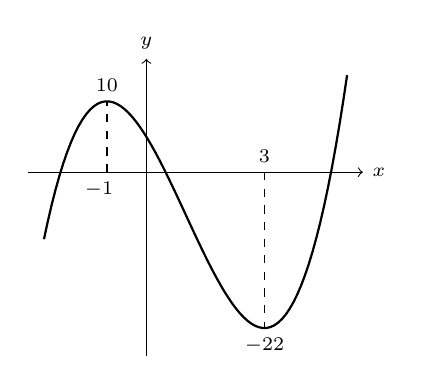
\begin{tikzpicture}[x=5mm,y=0.9mm]
\draw[->] (-3,0)--(5.5,0) node[right]{\scriptsize $x$};
\draw[->] (0,-26)--(0,16) node[above]{\scriptsize $y$};
\draw[thick,domain=-2.6:5.1,samples=80] plot (\x,{\x*\x*\x-3*\x*\x-9*\x+5});
\draw[dashed] (-1,0)--(-1,10) (3,0)--(3,-22);
\node[above] at (-1,10){\scriptsize 10}; \node[below] at (3,-22){\scriptsize $-22$};
\node[below] at (-1.2,0){\scriptsize $-1$}; \node[above] at (3,0){\scriptsize 3};
\end{tikzpicture}
\end{minipage}
\end{kai}

\ans{90}{共通接線}
\begin{kai}
\textbf{方針}\quad 求める直線を $y=mx+n$ とおき，\point{2つの放物線それぞれと連立した2次方程式がともに重解をもつ（判別式 $=0$）}条件を立てる．\\[2pt]
$y=x^2$ と $y=mx+n$ から\quad $x^2-mx-n=0$\\
\hspace*{1.5em}重解をもつ条件：$D_1=m^2+4n=0$ ……①\\
$y=-x^2+4x-4$ と $y=mx+n$ から\quad $x^2+(m-4)x+n+4=0$\\
\hspace*{1.5em}重解をもつ条件：$D_2=(m-4)^2-4(n+4)=0$ ……②\\[2pt]
①より $4n=-m^2$．②に代入して\\
\hspace*{1.5em}$(m-4)^2+m^2-16=0$，\quad $2m^2-8m=0$，\quad $2m(m-4)=0$，\quad $m=0,\ 4$\\
\hspace*{1.5em}$m=0$ のとき $n=0$，\quad $m=4$ のとき $n=-4$\\[2pt]
よって\quad $y=0$，\quad $y=4x-4$\\
（$y=0$ は $y=x^2$ と原点で，$y=-x^2+4x-4=-(x-2)^2$ と点 $(2,\ 0)$ で接する．）
\end{kai}

\ans{91}{関数決定（Ⅱ）}
\begin{kai}
\textbf{方針}\quad \point{$x=\alpha$ で極値をとるなら $f'(\alpha)=0$}（必要条件）．係数を求めたら，\point{本当にその点で極大・極小になるかを増減で確かめる}（十分性）．\\[2pt]
$f'(x)=3x^2+2ax+b$\\
$x=-1,\ 1$ で極値をとるので\quad $f'(-1)=3-2a+b=0$，\quad $f'(1)=3+2a+b=0$\\
2式を引いて $4a=0$，$a=0$．よって $b=-3$．\\
$f(-1)=5$ より\quad $-1+0+3+c=5$，\quad $c=3$\\[2pt]
\point{逆の確認}：このとき $f(x)=x^3-3x+3$，$f'(x)=3(x+1)(x-1)$．\\
\hspace*{1.5em}$f'(x)$ の符号は $x<-1$ で $+$，$-1<x<1$ で $-$，$x>1$ で $+$．\\
\hspace*{1.5em}$x=-1$ で極大，$x=1$ で極小となり条件をみたす．\\[2pt]
$a=0$，$b=-3$，$c=3$，\quad 極小値 $f(1)=1-3+3=1$
\end{kai}

\ans{92}{極値をもつための条件}
\begin{kai}
\textbf{方針}\quad 3次関数が極値をもつ ⇔ \point{$f'(x)$ の符号が変わる点がある ⇔ $f'(x)=0$ が異なる2つの実数解をもつ}．重解のときは符号が変わらないので極値をもたない．\\[2pt]
$f'(x)=3x^2+2ax+3$\\
$f'(x)=0$ が異なる2つの実数解をもつ条件は\quad $\dfrac D4=a^2-3\cdot3=a^2-9>0$\\
$(a+3)(a-3)>0$ より\quad $a<-3,\ 3<a$\\
\point{$D\geqq0$ としない．$D=0$ のとき $f'(x)\geqq0$ で単調増加になり，極値をもたない}
\end{kai}

\ans{93}{最大・最小}
\begin{kai}
\textbf{方針}\quad 増減を調べ，\point{極値と区間の端点の値をすべて比べる}．\\[2pt]
$f'(x)=3x^2-12x+9=3(x^2-4x+3)=3(x-1)(x-3)$\\
$0\leqq x\leqq4$ での増減：$0\leqq x<1$ で増加，$1<x<3$ で減少，$3<x\leqq4$ で増加．\\
\hspace*{1.5em}$f(0)=0$，\quad $f(1)=1-6+9=4$（極大），\quad $f(3)=27-54+27=0$（極小），\quad $f(4)=64-96+36=4$\\[2pt]
\point{極値と端点の値を比べる}\\
最大値 $4$\quad（$x=1,\ 4$），\quad 最小値 $0$\quad（$x=0,\ 3$）
\end{kai}

\ans{94}{最大値・最小値の図形への応用}
\begin{kai}
\textbf{方針}\quad 容積 $V$ を $x$ の式で表し，$x$ の動く範囲で増減表をかいて最大値を求める．\\[2pt]
箱の底面は1辺 $12-2x$ の正方形，高さは $x$ だから\quad $V=x(12-2x)^2$\\
\point{変数の範囲}\quad $x>0$ かつ $12-2x>0$ より\quad $0<x<6$\\[2pt]
$V'=(12-2x)^2+x\cdot2(12-2x)\cdot(-2)=(12-2x)\{(12-2x)-4x\}=(12-2x)(12-6x)=12(6-x)(2-x)$\\
$0<x<6$ では $6-x>0$ だから，$V'$ の符号は $2-x$ の符号と一致する．$V'=0$ となるのは $x=2$．
\begin{center}
\begin{tabular}{c|ccccc}
$x$ & $(0)$ & $\cdots$ & $2$ & $\cdots$ & $(6)$\\ \hline
$V'$ & & $+$ & $0$ & $-$ & \\ \hline
$V$ & & $\nearrow$ & $128$ & $\searrow$ &
\end{tabular}
\end{center}
$V(2)=2\cdot(12-4)^2=2\cdot64=128$\\
よって\quad $x=2$ のとき，最大値 $128$（cm$^3$）\\
\point{端の $x=0,\ 6$ は範囲に含まれない．増減表で「増加→減少」の切りかわりを確かめてから最大と答える}
\end{kai}

\ans{95}{微分法の方程式への応用}
\begin{kai}
\textbf{方針}\quad \point{定数 $a$ を分離して $x^3-3x=a$ とし，$y=x^3-3x$ のグラフと直線 $y=a$ の共有点の個数}を調べる．グラフは $a$ によらず固定なので考えやすい．\\[2pt]
$f(x)=x^3-3x$ とすると\quad $f'(x)=3x^2-3=3(x+1)(x-1)$\\
$x=-1$ で極大値 $f(-1)=-1+3=2$，\quad $x=1$ で極小値 $f(1)=1-3=-2$\\
$x\to\pm\infty$ で $f(x)\to\pm\infty$．\\[2pt]
直線 $y=a$（$x$ 軸に平行）を上下に動かして共有点の個数を数えると\\
\hspace*{1.5em}$a<-2,\ 2<a$ のとき\quad 1個\\
\hspace*{1.5em}$a=-2,\ 2$ のとき\quad 2個\quad （極値をとる点で接する）\\
\hspace*{1.5em}$-2<a<2$ のとき\quad 3個
\end{kai}

\ans{96}{接線の本数}
\begin{kai}
\textbf{方針}\quad 接点を $(t,\ f(t))$ とおいて接線が点 $(2,\ b)$ を通る条件を $t$ の方程式にする．\point{3次関数では接点が異なれば接線も異なるので，$t$ の実数解の個数＝接線の本数}．あとは類題95と同じく定数を分離する．\\[2pt]
$y'=3x^2-3$．接点を $(t,\ t^3-3t)$ とすると接線は\\
\hspace*{1.5em}$y=(3t^2-3)(x-t)+t^3-3t$\\
これが点 $(2,\ b)$ を通るので\\
\hspace*{1.5em}$b=(3t^2-3)(2-t)+t^3-3t=6t^2-3t^3-6+3t+t^3-3t=-2t^3+6t^2-6$\\[2pt]
$g(t)=-2t^3+6t^2-6$ とすると\quad $g'(t)=-6t^2+12t=-6t(t-2)$\\
\hspace*{1.5em}$t=0$ で極小値 $g(0)=-6$，\quad $t=2$ で極大値 $g(2)=-16+24-6=2$\\[2pt]
$y=g(t)$ のグラフと直線 $y=b$ が異なる3点で交わる条件は\quad $-6<b<2$
\end{kai}

\ans{97}{微分法の不等式への応用（Ⅰ）}
\begin{kai}
\textbf{方針}\quad \point{(左辺)$-$(右辺)$=f(x)$ とおき，$x\geqq0$ での $f(x)$ の最小値が0以上}であることを示す．\\[2pt]
$f(x)=x^3+4-3x^2=x^3-3x^2+4$ とすると\quad $f'(x)=3x^2-6x=3x(x-2)$\\
$x\geqq0$ での増減：$0<x<2$ で $f'(x)<0$（減少），$x>2$ で $f'(x)>0$（増加）．\\
よって $x\geqq0$ では，$x=2$ で最小値 $f(2)=8-12+4=0$ をとる．\\[2pt]
したがって $x\geqq0$ で $f(x)\geqq0$，すなわち\quad $x^3+4\geqq3x^2$\\
等号は $x=2$ のとき成りたつ．\\
（$f(x)=(x+1)(x-2)^2$ と因数分解できることからも確かめられる．）
\end{kai}

\ans{98}{微分法の不等式への応用（Ⅱ）}
\begin{kai}
\textbf{方針}\quad 「範囲内のすべての $x$ で $f(x)\geqq0$」 ⇔ \point{範囲内での $f(x)$ の最小値 $\geqq0$}．増減表から最小値を求める．\\[2pt]
$f(x)=x^3-3x+a$ とすると\quad $f'(x)=3x^2-3=3(x+1)(x-1)$\\
$x\geqq0$ での増減：$0<x<1$ で減少，$x>1$ で増加．\\
よって $x\geqq0$ での最小値は\quad $f(1)=1-3+a=a-2$\\[2pt]
\point{(最小値) $\geqq0$}\quad $a-2\geqq0$ より\quad $a\geqq2$
\end{kai}

\ans{99}{不定積分（Ⅰ）}
\begin{kai}
\textbf{方針}\quad \point{$\displaystyle\int x^n\,dx=\frac{x^{n+1}}{n+1}+C$}．積の形は\point{展開してから}積分する．\\[2pt]
（$C$ は積分定数）\\
(1)\ $\displaystyle\int(3x^2-4x+1)\,dx=3\cdot\frac{x^3}3-4\cdot\frac{x^2}2+x+C=x^3-2x^2+x+C$\\[2pt]
(2)\ $(2x+1)(x-3)=2x^2-6x+x-3=2x^2-5x-3$ だから\\
\hspace*{1.5em}$\displaystyle\int(2x^2-5x-3)\,dx=\frac23x^3-\frac52x^2-3x+C$\\
\hspace*{1.5em}（微分してもとの式にもどることで検算できる．）
\end{kai}

\ans{100}{不定積分（Ⅱ）}
\begin{kai}
\textbf{方針}\quad (1)は不定積分で $F(x)$ を求め，\point{条件 $F(1)=3$ で積分定数を決める}．(2)は\point{$(ax+b)^n$ の形のまま積分する公式}を使う（展開してもよい）．\\[2pt]
(1)\ $F(x)=\displaystyle\int(6x^2-2x)\,dx=2x^3-x^2+C$\\
\hspace*{1.5em}$F(1)=2-1+C=1+C=3$ より\quad $C=2$\\
\hspace*{1.5em}$F(x)=2x^3-x^2+2$\\[2pt]
(2)\ \point{$\displaystyle\int(ax+b)^n\,dx=\frac{(ax+b)^{n+1}}{a(n+1)}+C$}\\
\hspace*{1.5em}$\displaystyle\int(2x+3)^3\,dx=\frac{(2x+3)^4}{2\cdot4}+C=\frac{(2x+3)^4}{8}+C$\\
\hspace*{1.5em}（検算：$\left\{\dfrac{(2x+3)^4}{8}\right\}'=\dfrac{4(2x+3)^3\cdot2}{8}=(2x+3)^3$．$a=2$ で割るのを忘れない．）
\end{kai}

\ans{101}{定積分}
\begin{kai}
\textbf{方針}\quad 原始関数 $F(x)$ を求めて $\displaystyle\int_a^bf(x)\,dx=F(b)-F(a)$．区間が $-a$ から $a$ なら\point{奇数次の項は0，偶数次の項は $2\displaystyle\int_0^a$} で計算が楽になる．\\[2pt]
(1)\ $\displaystyle\int_0^3(x^2-2x+3)\,dx=\left[\frac{x^3}3-x^2+3x\right]_0^3=(9-9+9)-0=9$\\[2pt]
(2)\ $x^3$，$-x$ は奇関数（グラフが原点対称）なので，$-2$ から $2$ までの積分は0．\\
\hspace*{1.5em}$3x^2$，$1$ は偶関数（グラフが $y$ 軸対称）なので，$0$ から $2$ までの積分の2倍．\\
\hspace*{1.5em}$\displaystyle\int_{-2}^{2}(x^3+3x^2-x+1)\,dx=2\int_0^2(3x^2+1)\,dx=2\Bigl[x^3+x\Bigr]_0^2=2(8+2)=20$
\end{kai}

\ans{102}{絶対値記号のついた関数の定積分}
\begin{kai}
\textbf{方針}\quad \point{絶対値の中身の符号が変わる点で積分区間を分け}，絶対値をはずしてから積分する．\\[2pt]
(1)\ $|x-1|=\begin{cases}1-x & (0\leqq x\leqq1)\\ x-1 & (1\leqq x\leqq3)\end{cases}$\\[2pt]
\hspace*{1.5em}$\displaystyle\int_0^3|x-1|\,dx=\int_0^1(1-x)\,dx+\int_1^3(x-1)\,dx=\left[x-\frac{x^2}2\right]_0^1+\left[\frac{x^2}2-x\right]_1^3=\frac12+2=\frac52$\\
\hspace*{1.5em}（グラフで考えると，2つの直角二等辺三角形の面積 $\dfrac12+2$．）\\[2pt]
(2)\ $x^2-x-2=(x+1)(x-2)$ は，$0\leqq x\leqq2$ で0以下，$2\leqq x\leqq3$ で0以上．\\
\hspace*{1.5em}$\displaystyle\int_0^2(x^2-x-2)\,dx=\left[\frac{x^3}3-\frac{x^2}2-2x\right]_0^2=\frac83-2-4=-\frac{10}3$\\[2pt]
\hspace*{1.5em}$\displaystyle\int_2^3(x^2-x-2)\,dx=\left(9-\frac92-6\right)-\left(\frac83-2-4\right)=-\frac32+\frac{10}3=\frac{11}6$\\[2pt]
\hspace*{1.5em}$\displaystyle\int_0^3|x^2-x-2|\,dx=-\int_0^2(x^2-x-2)\,dx+\int_2^3(x^2-x-2)\,dx=\frac{10}3+\frac{11}6=\frac{31}6$
\end{kai}

\ans{103}{定積分で表された関数（Ⅰ）}
\begin{kai}
\textbf{方針}\quad \point{上端・下端が定数の定積分は定数なので $k$ とおく}．$f(x)$ を $k$ で表し，それを $k$ の定義式に代入して $k$ の方程式を解く．\\[2pt]
$\displaystyle k=\int_0^1f(t)\,dt$ とおくと\quad $f(x)=x^2+2k$\\
これを $k$ の式に代入して\\
\hspace*{1.5em}$\displaystyle k=\int_0^1(t^2+2k)\,dt=\left[\frac{t^3}3+2kt\right]_0^1=\frac13+2k$\\
よって $k=\dfrac13+2k$，\quad $k=-\dfrac13$\\[2pt]
$f(x)=x^2-\dfrac23$\\
（確認：$\displaystyle\int_0^1\left(t^2-\frac23\right)dt=\frac13-\frac23=-\frac13=k$）
\end{kai}

\ans{104}{定積分で表された関数（Ⅱ）}
\begin{kai}
\textbf{方針}\quad \point{$\dfrac{d}{dx}\displaystyle\int_a^xf(t)\,dt=f(x)$} なので，両辺を $x$ で微分すると $f(x)$ が求まる．\point{$x=a$ を代入すると左辺は0}になり，$a$ が求まる．\\[2pt]
両辺を $x$ で微分して\quad $f(x)=2x-3$\\[2pt]
与式に $x=a$ を代入すると，左辺は $\displaystyle\int_a^af(t)\,dt=0$ だから\\
\hspace*{1.5em}$0=a^2-3a+2=(a-1)(a-2)$\quad より\quad $a=1,\ 2$\\[2pt]
よって\quad $f(x)=2x-3$，\quad $a=1,\ 2$\\
（確認：$\displaystyle\int_1^x(2t-3)\,dt=\Bigl[t^2-3t\Bigr]_1^x=x^2-3x+2$．$a=2$ でも同じ式になる．）
\end{kai}

\ans{105}{面積（Ⅰ）}
\begin{kai}
\textbf{方針}\quad $x$ 軸との交点を求めて積分区間を決める．\point{曲線が $x$ 軸より下にある部分の面積は $-\displaystyle\int f(x)\,dx$}．\\[2pt]
$x^2-2x=x(x-2)=0$ より，$x$ 軸との交点は $x=0,\ 2$．\\
$0\leqq x\leqq2$ で $x^2-2x\leqq0$（グラフは $x$ 軸より下）だから\\[2pt]
$S=-\displaystyle\int_0^2(x^2-2x)\,dx=-\left[\frac{x^3}3-x^2\right]_0^2=-\left(\frac83-4\right)=\frac43$\\[2pt]
（公式 $\displaystyle\int_\alpha^\beta(x-\alpha)(x-\beta)\,dx=-\frac16(\beta-\alpha)^3$ を使うと $S=\dfrac16\cdot2^3=\dfrac43$．）
\end{kai}

\ans{106}{面積（Ⅱ）}
\begin{kai}
\textbf{方針}\quad 交点の $x$ 座標を求め，\point{(上の式)$-$(下の式) を交点から交点まで積分}する．放物線と直線で囲まれた部分は $\dfrac16$ 公式が使える．\\[2pt]
交点の $x$ 座標：$x^2=x+2$，$x^2-x-2=0$，$(x+1)(x-2)=0$ より\quad $x=-1,\ 2$\\
$-1\leqq x\leqq2$ では直線が放物線より上にあるので\\[2pt]
$S=\displaystyle\int_{-1}^2\{(x+2)-x^2\}\,dx=-\int_{-1}^2(x+1)(x-2)\,dx$\\[2pt]
\point{$\displaystyle\int_\alpha^\beta(x-\alpha)(x-\beta)\,dx=-\frac{(\beta-\alpha)^3}6$} を使うと\quad $S=\dfrac{\{2-(-1)\}^3}6=\dfrac{27}6=\dfrac92$\\
（直接計算：$\left[\dfrac{x^2}2+2x-\dfrac{x^3}3\right]_{-1}^2=\left(2+4-\dfrac83\right)-\left(\dfrac12-2+\dfrac13\right)=\dfrac{10}3+\dfrac76=\dfrac92$）
\end{kai}

\ans{107}{面積（Ⅲ）}
\begin{kai}
\textbf{方針}\quad 交点を求め，(上の式)$-$(下の式) を積分する．差が2次式になるので\point{$\dfrac16$ 公式}が使える．\\[2pt]
交点の $x$ 座標：$x^2=-x^2+4x$，$2x^2-4x=0$，$2x(x-2)=0$ より\quad $x=0,\ 2$\\
$0\leqq x\leqq2$ では $y=-x^2+4x$ が上にあるので\\[2pt]
$S=\displaystyle\int_0^2\{(-x^2+4x)-x^2\}\,dx=\int_0^2(-2x^2+4x)\,dx=-2\int_0^2x(x-2)\,dx$\\[2pt]
\hspace*{1.5em}$=-2\cdot\left(-\dfrac{2^3}6\right)=\dfrac83$\\
（直接計算：$\left[-\dfrac23x^3+2x^2\right]_0^2=-\dfrac{16}3+8=\dfrac83$）
\end{kai}

\ans{108}{面積（Ⅳ）}
\begin{kai}
\textbf{方針}\quad 2本の接線の式と交点を求める．\point{接線の交点で積分区間を分ける}．放物線と接線の差は $(x-\text{接点})^2$ の形になる．\\[2pt]
$y'=2x$．\\
$\ell_1$：点 $(-1,\ 1)$ で傾き $-2$ だから\quad $y=-2(x+1)+1=-2x-1$\\
$\ell_2$：点 $(2,\ 4)$ で傾き $4$ だから\quad $y=4(x-2)+4=4x-4$\\
$\ell_1$ と $\ell_2$ の交点：$-2x-1=4x-4$ より\quad $x=\dfrac12$\\[2pt]
\begin{center}
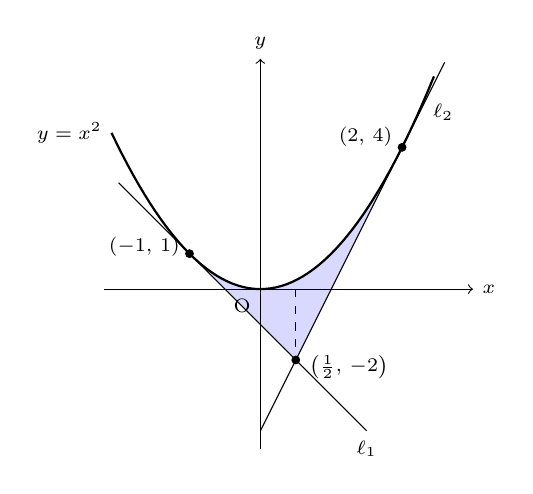
\begin{tikzpicture}[x=9mm,y=4.5mm]
\fill[blue!15] plot[domain=-1:2,samples=50] (\x,{\x*\x}) -- (0.5,-2) -- cycle;
\ax{-2.2}{3}{-4.5}{6.5}
\draw[thick,domain=-2.1:2.45,samples=60] plot (\x,{\x*\x});
\node[left] at (-2.1,4.4){\scriptsize $y=x^2$};
\draw (-2,3)--(1.5,-4) node[below]{\scriptsize $\ell_1$};
\draw (0,-4)--(2.6,6.4); \node[right] at (2.3,5){\scriptsize $\ell_2$};
\fill (-1,1) circle (1.6pt); \fill (2,4) circle (1.6pt); \fill (0.5,-2) circle (1.6pt);
\node[left] at (-1,1.2){\scriptsize $(-1,\,1)$}; \node[left] at (2,4.3){\scriptsize $(2,\,4)$};
\node[right] at (0.55,-2.2){\scriptsize $\left(\frac12,\,-2\right)$};
\draw[dashed] (0.5,0)--(0.5,-2);
\end{tikzpicture}
\end{center}
図の色の部分の面積を求める．$x=\dfrac12$ を境に，下側の線が $\ell_1$ から $\ell_2$ に変わる．\\[2pt]
放物線は接線より上にあり，$x^2-(-2x-1)=(x+1)^2$，$x^2-(4x-4)=(x-2)^2$ だから\\[2pt]
$S=\displaystyle\int_{-1}^{\frac12}(x+1)^2\,dx+\int_{\frac12}^2(x-2)^2\,dx=\left[\frac{(x+1)^3}3\right]_{-1}^{\frac12}+\left[\frac{(x-2)^3}3\right]_{\frac12}^2$\\[2pt]
\hspace*{1.5em}$=\dfrac13\left(\dfrac32\right)^3+\dfrac13\left(\dfrac32\right)^3=\dfrac{9}{8}+\dfrac98=\dfrac94$\\
\point{接線の交点の $x$ 座標は2接点の中点 $\dfrac{-1+2}2=\dfrac12$ になる}
\end{kai}

\ans{109}{面積（Ⅴ）}
\begin{kai}
\textbf{方針}\quad 接線の式を求め，曲線との交点を求める．\point{接点では重解になるので $(x-1)^2$ を因数にもつ}ことを使うと因数分解が楽．\\[2pt]
$y'=3x^2-3$ より，$x=1$ での傾きは0．接線は\quad $y=-2$\\[2pt]
曲線と接線の交点：$x^3-3x=-2$，$x^3-3x+2=0$\\
\hspace*{1.5em}$x=1$ で接するので $(x-1)^2$ を因数にもち\quad $(x-1)^2(x+2)=0$．他の交点は $x=-2$\\[2pt]
$-2\leqq x\leqq1$ では $(x-1)^2(x+2)\geqq0$ だから，曲線が接線より上にある．\\[2pt]
$S=\displaystyle\int_{-2}^1\{(x^3-3x)-(-2)\}\,dx=\int_{-2}^1(x^3-3x+2)\,dx=\left[\frac{x^4}4-\frac32x^2+2x\right]_{-2}^1$\\[2pt]
\hspace*{1.5em}$=\left(\dfrac14-\dfrac32+2\right)-(4-6-4)=\dfrac34+6=\dfrac{27}4$\\
（公式 $\displaystyle\int_\alpha^\beta(x-\alpha)(x-\beta)^2\,dx=\frac{(\beta-\alpha)^4}{12}$ を使うと $\dfrac{3^4}{12}=\dfrac{27}4$．）
\end{kai}

\ans{110}{面積（Ⅵ）}
\begin{kai}
\textbf{方針}\quad 全体の面積を求め，\point{直線 $y=mx$ と放物線で囲まれた部分の面積が全体の半分}になる条件を立てる．どちらも $\dfrac16$ 公式で計算できる．\\[2pt]
放物線 $y=2x-x^2=-x(x-2)$ と $x$ 軸で囲まれた部分の面積は\\
\hspace*{1.5em}$\displaystyle\int_0^2(2x-x^2)\,dx=\frac{2^3}6=\frac43$\\[2pt]
直線 $y=mx$ がこの部分を2つに分けるには，原点での接線の傾き2より小さく $0<m<2$．\\
放物線と直線の交点：$2x-x^2=mx$，$x\{x-(2-m)\}=0$ より\quad $x=0,\ 2-m$\\
直線と放物線で囲まれた部分の面積は\\
\hspace*{1.5em}$\displaystyle\int_0^{2-m}\{(2x-x^2)-mx\}\,dx=-\int_0^{2-m}x\{x-(2-m)\}\,dx=\frac{(2-m)^3}6$\\[2pt]
これが全体の半分 $\dfrac23$ に等しいので\quad $\dfrac{(2-m)^3}6=\dfrac23$，\quad $(2-m)^3=4$\\
$2-m=\sqrt[3]4$ より\quad $m=2-\sqrt[3]4$\quad （$0<m<2$ をみたす）
\end{kai}

\shouans{第7章}{数列}
\ans{111}{等差数列（Ⅰ）}
\begin{kai}
\textbf{方針}\quad \point{初項 $a$，公差 $d$ の等差数列の一般項は $a_n=a+(n-1)d$}．条件から $a,\ d$ の連立方程式をつくる．\\[2pt]
初項を $a$，公差を $d$ とすると\\
\hspace*{1.5em}$a_5=a+4d=11$ ……①，\quad $a_{12}=a+11d=32$ ……②\\
②$-$①より $7d=21$，$d=3$．①より $a=11-12=-1$．\\[2pt]
初項 $-1$，公差 $3$，\quad 一般項\quad $a_n=-1+3(n-1)=3n-4$\\
（確認：$a_5=11$，$a_{12}=32$）
\end{kai}

\ans{112}{等差数列（Ⅱ）}
\begin{kai}
\textbf{方針}\quad \point{等差数列の和 $S_n=\dfrac{n(a_1+a_n)}{2}=\dfrac{n\{2a+(n-1)d\}}{2}$}．(2)は最小・最大の7の倍数を求めて，公差7の等差数列とみる．\\[2pt]
(1)\ $S_{20}=\dfrac{20\{2\cdot2+(20-1)\cdot3\}}{2}=10\times61=610$\\[2pt]
(2)\ $100\div7=14$ 余り2 より，3桁の最小の7の倍数は $7\cdot15=105$．\\
\hspace*{1.5em}$999\div7=142$ 余り5 より，最大の7の倍数は $7\cdot142=994$．\\
\hspace*{1.5em}$7\cdot15,\ 7\cdot16,\ \cdots,\ 7\cdot142$ だから，個数は\quad $142-15+1=128$（個）\\
\hspace*{1.5em}これは初項105，末項994，項数128の等差数列なので，和は\\
\hspace*{1.5em}$\dfrac{128(105+994)}{2}=64\times1099=70336$
\end{kai}

\ans{113}{等差数列（Ⅲ）}
\begin{kai}
\textbf{方針}\quad 一般項を求めて $a_n<0$ を解く．公差が負の等差数列の和は，\point{正の項をすべて加えたところで最大}になる．\\[2pt]
(1)\ $a_n=47+(n-1)\cdot(-3)=50-3n$\\
\hspace*{1.5em}$a_n<0$ より $50-3n<0$，$n>\dfrac{50}3=16.6\cdots$．これをみたす最小の自然数は17．\quad 第17項\\[2pt]
(2)\ $a_{16}=50-48=2>0$，$a_{17}=50-51=-1<0$．\\
\hspace*{1.5em}第16項までは正の数を加えるので $S_n$ は増え，第17項以降は負の数を加えるので減る．\\
\hspace*{1.5em}よって $S_n$ が最大となるのは\quad $n=16$\\
\hspace*{1.5em}$S_{16}=\dfrac{16(a_1+a_{16})}2=\dfrac{16(47+2)}2=392$
\end{kai}

\ans{114}{等差数列（Ⅳ）}
\begin{kai}
\textbf{方針}\quad \point{等差数列をなす3数は $a-d,\ a,\ a+d$ とおく}と，和をとったとき $d$ が消えて計算が楽になる．\\[2pt]
3つの数を $a-d,\ a,\ a+d$ とおく．\\
和：$(a-d)+a+(a+d)=3a=15$ より\quad $a=5$\\
積：$(5-d)\cdot5\cdot(5+d)=5(25-d^2)=80$ より $25-d^2=16$，\quad $d^2=9$，\quad $d=\pm3$\\[2pt]
$d=3$ のとき $2,\ 5,\ 8$，\quad $d=-3$ のとき $8,\ 5,\ 2$\\
どちらも同じ3数なので，3つの数は\quad $2,\ 5,\ 8$
\end{kai}

\ans{115}{等比数列（Ⅰ）}
\begin{kai}
\textbf{方針}\quad \point{初項 $a$，公比 $r$ の等比数列の一般項は $a_n=ar^{n-1}$}．条件の2式を\point{割り算して $a$ を消去}する．\\[2pt]
初項を $a$，公比を $r$ とすると\\
\hspace*{1.5em}$a_2=ar=6$ ……①，\quad $a_5=ar^4=162$ ……②\\
②÷①より\quad $r^3=27$\\
$r$ は実数だから\quad $r=3$．①より $a=2$．\\[2pt]
一般項は\quad $a_n=2\cdot3^{n-1}$\\
（$r^3=27$ の虚数解 $r=\dfrac{-3\pm3\sqrt3\,i}{2}$ は「公比は実数」の条件で除かれる．）
\end{kai}

\ans{116}{等比数列（Ⅱ）}
\begin{kai}
\textbf{方針}\quad \point{等比数列の和 $S_n=\dfrac{a(r^n-1)}{r-1}$（$r\neq1$）}．(2)は不等式を $2^n$ について解き，2の累乗の値と比べる．\\[2pt]
(1)\ $S_{10}=\dfrac{3(2^{10}-1)}{2-1}=3(1024-1)=3069$\\[2pt]
(2)\ $S_n=\dfrac{3(2^n-1)}{2-1}=3(2^n-1)$．$S_n>1000$ より\\
\hspace*{1.5em}$2^n-1>\dfrac{1000}3=333.3\cdots$，\quad $2^n>334.3\cdots$\\
\hspace*{1.5em}$2^8=256<334.3$，\quad $2^9=512>334.3$ だから，初めて超えるのは\quad $n=9$\\
\hspace*{1.5em}（確認：$S_8=3\cdot255=765$，$S_9=3\cdot511=1533$）
\end{kai}

\ans{117}{等差中項・等比中項}
\begin{kai}
\textbf{方針}\quad \point{$a,\ b,\ c$ がこの順に等差数列 $\iff2b=a+c$，等比数列 $\iff b^2=ac$}（中項の性質）．順番に注意して式を立てる．\\[2pt]
$a,\ 4,\ b$ が等差数列だから\quad $2\cdot4=a+b$，\quad $a+b=8$ ……①\\
$4,\ b,\ a$ が等比数列だから\quad $b^2=4a$ ……②\\[2pt]
①より $a=8-b$．②に代入して\quad $b^2=4(8-b)$，\quad $b^2+4b-32=0$，\quad $(b+8)(b-4)=0$\\
\hspace*{1.5em}$b=4$ のとき $a=4$，\quad $b=-8$ のとき $a=16$\\[2pt]
よって\quad $(a,\ b)=(4,\ 4),\ (16,\ -8)$\\
（確認：$16,\ 4,\ -8$ は公差 $-12$，$4,\ -8,\ 16$ は公比 $-2$．）
\end{kai}

\ans{118}{$\Sigma$ 記号を用いた和の計算（Ⅰ）}
\begin{kai}
\textbf{方針}\quad \point{$\displaystyle\sum_{k=1}^nk=\frac{n(n+1)}2$，$\displaystyle\sum_{k=1}^nk^2=\frac{n(n+1)(2n+1)}6$，$\displaystyle\sum_{k=1}^nc=nc$}．展開して項ごとに分け，最後は共通因数でくくって整理する．\\[2pt]
(1)\ $\displaystyle\sum_{k=1}^n(2k-1)=2\sum_{k=1}^nk-\sum_{k=1}^n1=2\cdot\frac{n(n+1)}2-n=n^2+n-n=n^2$\\
\hspace*{1.5em}（1から始まる奇数を $n$ 個足すと $n^2$．）\\[2pt]
(2)\ $k(k+1)=k^2+k$ だから\\
\hspace*{1.5em}$\displaystyle\sum_{k=1}^nk(k+1)=\frac{n(n+1)(2n+1)}6+\frac{n(n+1)}2=\frac{n(n+1)}6\{(2n+1)+3\}$\\
\hspace*{1.5em}$=\dfrac{n(n+1)(2n+4)}6=\dfrac{n(n+1)(n+2)}3$\\
\hspace*{1.5em}（確認：$n=2$ のとき $1\cdot2+2\cdot3=8$，公式 $\dfrac{2\cdot3\cdot4}3=8$）
\end{kai}

\ans{119}{$\Sigma$ 記号を用いた和の計算（Ⅱ）}
\begin{kai}
\textbf{方針}\quad $\displaystyle\sum_{k=1}^nr^k$ は\point{初項 $r$，公比 $r$，項数 $n$ の等比数列の和}．初項が $r^1$ であることに注意する．\\[2pt]
(1)\ $\displaystyle\sum_{k=1}^n3^k=3+3^2+\cdots+3^n$ は，初項3，公比3，項数 $n$ の等比数列の和だから\\
\hspace*{1.5em}$\dfrac{3(3^n-1)}{3-1}=\dfrac{3(3^n-1)}2=\dfrac{3^{n+1}-3}2$\\[2pt]
(2)\ $\displaystyle\sum_{k=1}^n(k^2+2^k)=\sum_{k=1}^nk^2+\sum_{k=1}^n2^k$\\
\hspace*{1.5em}$\displaystyle\sum_{k=1}^n2^k$ は初項2，公比2，項数 $n$ の等比数列の和で $\dfrac{2(2^n-1)}{2-1}=2^{n+1}-2$\\
\hspace*{1.5em}よって\quad $\dfrac{n(n+1)(2n+1)}6+2^{n+1}-2$
\end{kai}

\ans{120}{$\Sigma$ 記号を用いた和の計算（Ⅲ）}
\begin{kai}
\textbf{方針}\quad \point{部分分数に分けて，隣り合う項を打ち消す}．$\dfrac1{AB}=\dfrac1{B-A}\left(\dfrac1A-\dfrac1B\right)$ を使う．\\[2pt]
(1)\ $\dfrac1{k(k+1)}=\dfrac1k-\dfrac1{k+1}$ だから\\
\hspace*{1.5em}$\displaystyle\sum_{k=1}^n\frac1{k(k+1)}$\\
\hspace*{3em}$\displaystyle=\left(\frac11-\frac12\right)+\left(\frac12-\frac13\right)+\cdots+\left(\frac1n-\frac1{n+1}\right)$\\
\hspace*{1.5em}途中が打ち消しあって最初と最後だけが残り\quad $=1-\dfrac1{n+1}=\dfrac n{n+1}$\\[2pt]
(2)\ $(2k+1)-(2k-1)=2$ だから\quad $\dfrac1{(2k-1)(2k+1)}=\dfrac12\left(\dfrac1{2k-1}-\dfrac1{2k+1}\right)$\\
\hspace*{1.5em}$\displaystyle\sum_{k=1}^n\frac1{(2k-1)(2k+1)}$\\
\hspace*{3em}$\displaystyle=\frac12\biggl\{\left(\frac11-\frac13\right)+\left(\frac13-\frac15\right)+\cdots+\left(\frac1{2n-1}-\frac1{2n+1}\right)\biggr\}$\\
\hspace*{1.5em}$=\dfrac12\left(1-\dfrac1{2n+1}\right)=\dfrac12\cdot\dfrac{2n}{2n+1}=\dfrac n{2n+1}$\\
\hspace*{1.5em}\point{係数 $\dfrac12$ を忘れない．分けた式を通分して検算するとよい}
\end{kai}

\ans{121}{$\Sigma$ 記号を用いた和の計算（Ⅳ）}
\begin{kai}
\textbf{方針}\quad \point{(等差数列)×(等比数列) の和は，公比 $r$ を掛けた $rS$ との差 $S-rS$ をつくる}と，等比数列の和に帰着する．\\[2pt]
$S_n=1\cdot2+2\cdot2^2+3\cdot2^3+\cdots+n\cdot2^n$\\
$2S_n=\phantom{1\cdot2+{}}1\cdot2^2+2\cdot2^3+\cdots+(n-1)\cdot2^n+n\cdot2^{n+1}$\\[2pt]
上の式から下の式を引くと（$2^k$ の係数をそろえて引く）\\
\hspace*{1.5em}$S_n-2S_n=2+2^2+2^3+\cdots+2^n-n\cdot2^{n+1}$\\
\hspace*{1.5em}$-S_n=\dfrac{2(2^n-1)}{2-1}-n\cdot2^{n+1}=2^{n+1}-2-n\cdot2^{n+1}=(1-n)2^{n+1}-2$\\[2pt]
よって\quad $S_n=(n-1)2^{n+1}+2$\\
（確認：$n=2$ のとき $2+8=10$，公式 $1\cdot8+2=10$）
\end{kai}

\ans{122}{階差数列}
\begin{kai}
\textbf{方針}\quad 差をとった数列（階差数列）$b_n=a_{n+1}-a_n$ の規則を見つける．\point{$n\geqq2$ のとき $a_n=a_1+\displaystyle\sum_{k=1}^{n-1}b_k$}．最後に $n=1$ でも成りたつか確かめる．\\[2pt]
階差数列は $2-1,\ 5-2,\ 10-5,\ 17-10,\ \cdots$ より\quad $1,\ 3,\ 5,\ 7,\ \cdots$\\
これは初項1，公差2の等差数列で，第 $k$ 項は $b_k=2k-1$．\\[2pt]
$n\geqq2$ のとき\\
\hspace*{1.5em}$a_n=1+\displaystyle\sum_{k=1}^{n-1}(2k-1)=1+(n-1)^2=n^2-2n+2$\\
\hspace*{1.5em}（類題118(1)より，1から始まる奇数 $n-1$ 個の和は $(n-1)^2$）\\
$n=1$ のとき $1-2+2=1=a_1$ で成りたつ．\\[2pt]
よって\quad $a_n=n^2-2n+2$
\end{kai}

\ans{123}{2項間の漸化式（Ⅰ）}
\begin{kai}
\textbf{方針}\quad $a_{n+1}-a_n=4n$ だから，\point{階差数列が $4n$ の数列}．$a_n=a_1+\displaystyle\sum_{k=1}^{n-1}4k$（$n\geqq2$）で求める．\\[2pt]
$a_{n+1}-a_n=4n$ より，$\{a_n\}$ の階差数列の第 $n$ 項は $4n$．\\
$n\geqq2$ のとき\\
\hspace*{1.5em}$a_n=3+\displaystyle\sum_{k=1}^{n-1}4k=3+4\cdot\frac{(n-1)n}2=3+2n(n-1)=2n^2-2n+3$\\
\hspace*{1.5em}\point{$\displaystyle\sum_{k=1}^{n-1}k=\frac{(n-1)n}2$．$n$ を $n-1$ におきかえる}\\
$n=1$ のとき $2-2+3=3=a_1$ で成りたつ．\\[2pt]
よって\quad $a_n=2n^2-2n+3$
\end{kai}

\ans{124}{2項間の漸化式（Ⅱ）}
\begin{kai}
\textbf{方針}\quad $a_{n+1}=pa_n+q$ 型は，\point{$\alpha=p\alpha+q$ をみたす $\alpha$ を引いて $a_{n+1}-\alpha=p(a_n-\alpha)$ と変形}する．$\{a_n-\alpha\}$ が等比数列になる．\\[2pt]
$\alpha=3\alpha+2$ を解くと\quad $\alpha=-1$\\
漸化式から $\alpha=3\alpha+2$ を辺々引くと\quad $a_{n+1}-\alpha=3(a_n-\alpha)$，すなわち\\
\hspace*{1.5em}$a_{n+1}+1=3(a_n+1)$\\
よって数列 $\{a_n+1\}$ は，初項 $a_1+1=2$，公比3の等比数列．\\
\hspace*{1.5em}$a_n+1=2\cdot3^{n-1}$\\[2pt]
よって\quad $a_n=2\cdot3^{n-1}-1$\\
（確認：$a_2=3\cdot1+2=5$，公式 $2\cdot3-1=5$）
\end{kai}

\ans{125}{2項間の漸化式（Ⅲ）}
\begin{kai}
\textbf{方針}\quad $3^n$ がじゃまなので，\point{両辺を $3^{n+1}$ で割って $b_n=\dfrac{a_n}{3^n}$ の漸化式}にすると，$b_{n+1}=pb_n+q$ 型になる．\\[2pt]
漸化式の両辺を $3^{n+1}$ で割ると\\
\hspace*{1.5em}$\dfrac{a_{n+1}}{3^{n+1}}=\dfrac23\cdot\dfrac{a_n}{3^n}+\dfrac{3^n}{3^{n+1}}$，\quad すなわち\quad $b_{n+1}=\dfrac23b_n+\dfrac13$\\[2pt]
$\alpha=\dfrac23\alpha+\dfrac13$ より $\alpha=1$．よって\quad $b_{n+1}-1=\dfrac23(b_n-1)$\\
$b_1=\dfrac{a_1}3=\dfrac13$ より $b_1-1=-\dfrac23$．$\{b_n-1\}$ は初項 $-\dfrac23$，公比 $\dfrac23$ の等比数列で\\
\hspace*{1.5em}$b_n-1=-\dfrac23\left(\dfrac23\right)^{n-1}=-\left(\dfrac23\right)^n$，\quad $b_n=1-\left(\dfrac23\right)^n$\\[2pt]
$a_n=3^nb_n=3^n-3^n\cdot\dfrac{2^n}{3^n}=3^n-2^n$\\
（確認：$a_2=2\cdot1+3=5$，公式 $9-4=5$）
\end{kai}

\ans{126}{2項間の漸化式（Ⅳ）}
\begin{kai}
\textbf{方針}\quad 分数型の漸化式は，\point{両辺の逆数をとる}と等差数列などの扱いやすい形になる．逆数をとる前に $a_n\neq0$ を確認する．\\[2pt]
$a_1=1>0$ で，$a_n>0$ なら $a_{n+1}=\dfrac{a_n}{2a_n+1}>0$．よってすべての $n$ で $a_n>0$（特に $a_n\neq0$）．\\[2pt]
両辺の逆数をとって\quad $\dfrac1{a_{n+1}}=\dfrac{2a_n+1}{a_n}=2+\dfrac1{a_n}$\\
$c_n=\dfrac1{a_n}$ とおくと $c_{n+1}=c_n+2$ で，$\{c_n\}$ は初項 $c_1=1$，公差2の等差数列．\\
\hspace*{1.5em}$c_n=1+2(n-1)=2n-1$\\[2pt]
よって\quad $a_n=\dfrac1{2n-1}$
\end{kai}

\ans{127}{2項間の漸化式（Ⅴ）}
\begin{kai}
\textbf{方針}\quad $a_{n+1}=pa_n+(n\text{の1次式})$ 型は，\point{$a_n+\alpha n+\beta$ が等比数列になるように $\alpha,\ \beta$ を決める}．\\[2pt]
(1)\ $a_{n+1}+\alpha(n+1)+\beta=2(a_n+\alpha n+\beta)$ を $a_{n+1}$ について解くと\\
\hspace*{1.5em}$a_{n+1}=2a_n+2\alpha n+2\beta-\alpha n-\alpha-\beta=2a_n+\alpha n+(\beta-\alpha)$\\
\hspace*{1.5em}これが $a_{n+1}=2a_n+n$ と一致するように，係数を比べて\quad $\alpha=1$，\quad $\beta-\alpha=0$\\
\hspace*{1.5em}よって\quad $\alpha=1$，$\beta=1$\\[2pt]
(2)\ (1)より\quad $a_{n+1}+(n+1)+1=2(a_n+n+1)$\\
\hspace*{1.5em}$\{a_n+n+1\}$ は，初項 $a_1+1+1=3$，公比2の等比数列．\\
\hspace*{1.5em}$a_n+n+1=3\cdot2^{n-1}$\\
\hspace*{1.5em}よって\quad $a_n=3\cdot2^{n-1}-n-1$\\
\hspace*{1.5em}（確認：$a_2=2\cdot1+1=3$，公式 $6-2-1=3$）
\end{kai}

\ans{128}{和と一般項}
\begin{kai}
\textbf{方針}\quad \point{$a_1=S_1$，$n\geqq2$ のとき $a_n=S_n-S_{n-1}$}．$n\geqq2$ で求めた式が $n=1$ でも成りたつかを必ず確かめる．\\[2pt]
$a_1=S_1=1+2+1=4$\\[2pt]
$n\geqq2$ のとき\\
\hspace*{1.5em}$a_n=S_n-S_{n-1}=(n^2+2n+1)-\{(n-1)^2+2(n-1)+1\}$\\
\hspace*{1.5em}$=(n^2+2n+1)-(n^2-2n+1+2n-2+1)=(n^2+2n+1)-n^2=2n+1$\\[2pt]
\point{$n=1$ のとき $2n+1=3\neq a_1$} なので，1つの式にはまとめられない．\\
よって\quad $a_1=4$，\quad $a_n=2n+1\ (n\geqq2)$\\
（$S_n$ に定数項1があるため，$a_1$ だけずれる．）
\end{kai}

\ans{129}{3項間の漸化式}
\begin{kai}
\textbf{方針}\quad $a_{n+2}=pa_{n+1}+qa_n$ 型は，\point{特性方程式 $t^2=pt+q$ の解 $\alpha,\ \beta$ を使って $a_{n+2}-\alpha a_{n+1}=\beta(a_{n+1}-\alpha a_n)$ と変形}する．\\[2pt]
特性方程式 $t^2=4t-3$，$t^2-4t+3=0$，$(t-1)(t-3)=0$ より\quad $t=1,\ 3$\\
$\alpha=1$，$\beta=3$ として変形すると\quad $a_{n+2}-a_{n+1}=3(a_{n+1}-a_n)$\\
（確認：展開すると $a_{n+2}=4a_{n+1}-3a_n$ にもどる．）\\[2pt]
階差数列 $\{a_{n+1}-a_n\}$ は，初項 $a_2-a_1=2$，公比3の等比数列．\\
\hspace*{1.5em}$a_{n+1}-a_n=2\cdot3^{n-1}$\\
$n\geqq2$ のとき\\
\hspace*{1.5em}$a_n=1+\displaystyle\sum_{k=1}^{n-1}2\cdot3^{k-1}=1+\frac{2(3^{n-1}-1)}{3-1}=3^{n-1}$\\
$n=1$ のとき $3^0=1=a_1$ で成りたつ．\\[2pt]
よって\quad $a_n=3^{n-1}$
\end{kai}

\ans{130}{連立型漸化式}
\begin{kai}
\textbf{方針}\quad 係数が対称な連立漸化式は，\point{2式の和と差をつくる}と，それぞれが等比数列になる．最後に連立して $a_n,\ b_n$ を求める．\\[2pt]
2式を辺々加えると\quad $a_{n+1}+b_{n+1}=3a_n+3b_n=3(a_n+b_n)$\\
2式を辺々引くと\quad $a_{n+1}-b_{n+1}=-a_n+b_n=-(a_n-b_n)$\\[2pt]
$\{a_n+b_n\}$ は初項 $a_1+b_1=3$，公比3の等比数列で\quad $a_n+b_n=3\cdot3^{n-1}=3^n$ ……①\\
$\{a_n-b_n\}$ は初項 $a_1-b_1=-1$，公比 $-1$ の等比数列で\quad $a_n-b_n=(-1)\cdot(-1)^{n-1}=(-1)^n$ ……②\\[2pt]
(①＋②)÷2，(①－②)÷2 より\\
\hspace*{1.5em}$a_n=\dfrac{3^n+(-1)^n}2$，\quad $b_n=\dfrac{3^n-(-1)^n}2$\\
（確認：$n=1$ のとき $a_1=\dfrac{3-1}2=1$，$b_1=\dfrac{3+1}2=2$）
\end{kai}

\ans{131}{群数列（Ⅰ）}
\begin{kai}
\textbf{方針}\quad 群数列は\point{第 $k$ 群の項数を調べ，第 $n-1$ 群までの項数の合計を求める}．第 $n$ 群の最初の数は「それまでの個数 $+1$」番目．\\[2pt]
(1)\ 第 $k$ 群には $k$ 個の数がある．第1群から第 $(n-1)$ 群までの数の個数は\\
\hspace*{1.5em}$1+2+\cdots+(n-1)=\dfrac{(n-1)n}2$\\
\hspace*{1.5em}自然数が順に並んでいるので，第 $(n-1)$ 群の末項は $\dfrac{n(n-1)}2$．よって第 $n$ 群の最初の数は\\
\hspace*{1.5em}$\dfrac{n(n-1)}2+1$\quad （$n\geqq2$．$n=1$ のときも1で成りたつ）\\[2pt]
(2)\ 第 $m$ 群の末項は $\dfrac{m(m+1)}2$．$\dfrac{m(m+1)}2\geqq100$ となる最小の $m$ を探す．\\
\hspace*{1.5em}$m=13$ のとき $\dfrac{13\cdot14}2=91$，\quad $m=14$ のとき $\dfrac{14\cdot15}2=105$\\
\hspace*{1.5em}$91<100\leqq105$ だから，100は第14群にある．$100-91=9$ より\quad 第14群の9番目
\end{kai}

\ans{132}{群数列（Ⅱ）}
\begin{kai}
\textbf{方針}\quad \point{分母が同じものを1つの群にまとめる}．第 $k$ 群は $\dfrac1k,\ \dfrac2k,\ \cdots,\ \dfrac kk$ の $k$ 項．何番目の項が第何群の何番目かを調べる．\\[2pt]
分母が $k$ の項を第 $k$ 群とすると，第 $k$ 群は $k$ 項．\\
第 $m$ 群までの項数は $\dfrac{m(m+1)}2$ で，$m=9$ のとき45，$m=10$ のとき55．\\[2pt]
(1)\ $45<50\leqq55$ だから，第50項は第10群の $50-45=5$ 番目．\quad $\dfrac5{10}=\dfrac12$\\[2pt]
(2)\ 第 $k$ 群の和は\quad $\dfrac{1+2+\cdots+k}{k}=\dfrac{1}{k}\cdot\dfrac{k(k+1)}2=\dfrac{k+1}2$\\
\hspace*{1.5em}第1群から第9群までの和：$\displaystyle\sum_{k=1}^9\frac{k+1}2=\frac12\left(\frac{9\cdot10}2+9\right)=\frac{54}2=27$\\
\hspace*{1.5em}第10群の1番目から5番目までの和：$\dfrac{1+2+3+4+5}{10}=\dfrac{15}{10}=\dfrac32$\\
\hspace*{1.5em}合計\quad $27+\dfrac32=\dfrac{57}2$
\end{kai}

\ans{133}{格子点の個数}
\begin{kai}
\textbf{方針}\quad \point{直線 $y=k$（$k$ は整数）上の格子点を数えて，$k$ について加える}．$x$ の範囲が $y$ によって変わるので，$y$ を固定する方が数えやすい．\\[2pt]
$y\geqq0$，$x\geqq0$ と $x+2y\leqq2n$ から，$y$ のとりうる整数値は $0\leqq y\leqq n$．\\
直線 $y=k$（$k=0,\ 1,\ \cdots,\ n$）上では $0\leqq x\leqq2n-2k$ だから，格子点は\quad $2n-2k+1$ 個\\[2pt]
総数は\\
\hspace*{1.5em}$\displaystyle\sum_{k=0}^n(2n-2k+1)=(2n+1)(n+1)-2\sum_{k=0}^nk=(2n+1)(n+1)-n(n+1)$\\
\hspace*{1.5em}$=(n+1)(2n+1-n)=(n+1)^2$（個）\\
\point{$k=0$ から始まるので項数は $n+1$ 個}\\
（確認：$n=1$ のとき $(0,0),(1,0),(2,0),(0,1)$ の4個 $=2^2$）
\end{kai}

\ans{134}{漸化式の応用}
\begin{kai}
\textbf{方針}\quad \point{$n$ 本の状態に1本加えたとき，部分がいくつ増えるか}を考えて漸化式をつくる．新しい直線は，他の直線との交点で区切られた各部分ごとに，領域を1つずつ2つに分ける．\\[2pt]
(1)\ $(n+1)$ 本目の直線は，他の $n$ 本とそれぞれ1点で交わり，交点はすべて異なる（どの3本も1点で交わらない）．\\
\hspace*{1.5em}よって $(n+1)$ 本目の直線は $n$ 個の交点で $n+1$ 個の部分（線分と半直線）に分けられる．\\
\hspace*{1.5em}その各部分が，それが通る領域を2つに分けるので，領域は $n+1$ 個増える．\\
\hspace*{1.5em}$a_{n+1}=a_n+n+1$\\[2pt]
(2)\ 1本の直線は平面を2つに分けるので $a_1=2$．階差数列が $n+1$ だから，$n\geqq2$ のとき\\
\hspace*{1.5em}$a_n=2+\displaystyle\sum_{k=1}^{n-1}(k+1)=2+\frac{(n-1)n}2+(n-1)=\frac{n^2+n+2}2$\\
\hspace*{1.5em}$n=1$ のとき $\dfrac{1+1+2}2=2$ で成りたつ．\quad よって\quad $a_n=\dfrac{n^2+n+2}2$\\
\hspace*{1.5em}（確認：$a_2=4$，$a_3=7$）
\end{kai}

\ans{135}{場合の数と漸化式}
\begin{kai}
\textbf{方針}\quad \point{最後（右端）に置くタイルで場合分け}すると，残りの部分は長さの短い同じ問題になり，漸化式ができる．\\[2pt]
(1)\ $n=1$：横1のタイル1枚だけ．\quad $a_1=1$\\
\hspace*{1.5em}$n=2$：横1を2枚，または横2を1枚．\quad $a_2=2$\\[2pt]
\hspace*{1.5em}横 $n+2$ の長方形について，右端に置くタイルで場合分けする．\\
\hspace*{1.5em}右端が横1のタイルのとき，残りは横 $n+1$ の長方形で\quad $a_{n+1}$ 通り\\
\hspace*{1.5em}右端が横2のタイルのとき，残りは横 $n$ の長方形で\quad $a_n$ 通り\\
\hspace*{1.5em}この2つは重複しないので\quad $a_{n+2}=a_{n+1}+a_n$\\[2pt]
(2)\ 漸化式を順に使って\\
\hspace*{1.5em}$a_3=2+1=3$，$a_4=3+2=5$，$a_5=5+3=8$，$a_6=8+5=13$，$a_7=13+8=21$，$a_8=21+13=34$\\
\hspace*{1.5em}よって\quad $a_8=34$\quad （フィボナッチ数列になっている）
\end{kai}

\ans{136}{確率と漸化式}
\begin{kai}
\textbf{方針}\quad \point{$n$ 回目までの状態（偶数回か奇数回か）と $(n+1)$ 回目の結果で場合分け}して漸化式をつくる．$p_{n+1}=ap_n+b$ 型を解く．\\[2pt]
(1)\ $(n+1)$ 回投げて1の目が偶数回になるのは，次の2つの場合（互いに排反）．\\
\hspace*{1.5em}(i)\ $n$ 回目までに偶数回で，$(n+1)$ 回目に1以外が出る：確率\quad $p_n\times\dfrac56$\\
\hspace*{1.5em}(ii)\ $n$ 回目までに奇数回で，$(n+1)$ 回目に1が出る：確率\quad $(1-p_n)\times\dfrac16$\\
\hspace*{1.5em}よって\quad $p_{n+1}=\dfrac56p_n+\dfrac16(1-p_n)=\dfrac23p_n+\dfrac16$\\[2pt]
(2)\ $\alpha=\dfrac23\alpha+\dfrac16$ より $\alpha=\dfrac12$．\quad $p_{n+1}-\dfrac12=\dfrac23\left(p_n-\dfrac12\right)$\\
\hspace*{1.5em}$p_1$ は1回投げて1が0回（1以外が出る）確率で $p_1=\dfrac56$．$p_1-\dfrac12=\dfrac13$．\\
\hspace*{1.5em}$p_n-\dfrac12=\dfrac13\left(\dfrac23\right)^{n-1}=\dfrac12\left(\dfrac23\right)^n$\\
\hspace*{1.5em}よって\quad $p_n=\dfrac12+\dfrac12\left(\dfrac23\right)^n$\\
\hspace*{1.5em}（$n$ が大きくなると $p_n$ は $\dfrac12$ に近づく．）
\end{kai}

\ans{137}{数学的帰納法（Ⅰ）}
\begin{kai}
\textbf{方針}\quad 数学的帰納法：\point{[1] $n=1$ で成りたつ，[2] $n=k$ で成りたつと仮定して $n=k+1$ で成りたつ}，の2つを示す．[2]では仮定の式を必ず使う．\\[2pt]
{[1]}\ $n=1$ のとき，左辺 $=1\cdot2=2$，右辺 $=\dfrac{1\cdot2\cdot3}3=2$ で成りたつ．\\[2pt]
{[2]}\ $n=k$ のとき成りたつと仮定すると\quad $1\cdot2+2\cdot3+\cdots+k(k+1)=\dfrac{k(k+1)(k+2)}3$\\
\hspace*{1.5em}$n=k+1$ のときの左辺は，これに $(k+1)(k+2)$ を加えたものだから\\
\hspace*{1.5em}左辺 $=\dfrac{k(k+1)(k+2)}3+(k+1)(k+2)=\dfrac{(k+1)(k+2)(k+3)}3$\\
\hspace*{1.5em}（$(k+1)(k+2)$ でくくると $\dfrac{k}{3}+1=\dfrac{k+3}3$）\\
\hspace*{1.5em}これは $n=k+1$ のときの右辺 $\dfrac{(k+1)\{(k+1)+1\}\{(k+1)+2\}}3$ に等しい．よって $n=k+1$ でも成りたつ．\\[2pt]
{[1]}，[2]より，すべての自然数 $n$ について等式は成りたつ．
\end{kai}

\ans{138}{数学的帰納法（Ⅱ）}
\begin{kai}
\textbf{方針}\quad 出発点が $n=5$ の数学的帰納法．[2]では，仮定 $2^k>k^2$ から $2^{k+1}>2k^2$ を導き，\point{$2k^2\geqq(k+1)^2$（$k\geqq5$）を示してつなぐ}．\\[2pt]
{[1]}\ $n=5$ のとき，$2^5=32$，$5^2=25$ で $32>25$．成りたつ．\\[2pt]
{[2]}\ $k\geqq5$ として，$n=k$ のとき成りたつ，すなわち $2^k>k^2$ と仮定する．\\
\hspace*{1.5em}両辺を2倍して\quad $2^{k+1}>2k^2$ ……①\\
\hspace*{1.5em}ここで\quad $2k^2-(k+1)^2=k^2-2k-1=(k-1)^2-2$\\
\hspace*{1.5em}$k\geqq5$ より $(k-1)^2\geqq16$ だから $(k-1)^2-2>0$，すなわち $2k^2>(k+1)^2$ ……②\\
\hspace*{1.5em}①，②より\quad $2^{k+1}>(k+1)^2$．よって $n=k+1$ でも成りたつ．\\[2pt]
{[1]}，[2]より，$n\geqq5$ をみたすすべての自然数 $n$ について $2^n>n^2$ は成りたつ．\\
（$n=2,\ 3,\ 4$ では成りたたない：$4=4$，$8<9$，$16=16$．）
\end{kai}

\shouans{第8章}{ベクトル}
\ans{139}{$m\vec a+n\vec b$}
\begin{kai}
\textbf{方針}\quad 成分で $m\vec a+n\vec b$ を計算し，\point{$x$ 成分，$y$ 成分をそれぞれ比較}して $m,\ n$ の連立方程式を解く．\\[2pt]
$m\vec a+n\vec b=m(2,\ 1)+n(-1,\ 3)=(2m-n,\ m+3n)$\\
これが $(7,\ 0)$ に等しいので\quad $2m-n=7$ ……①，\quad $m+3n=0$ ……②\\
②より $m=-3n$．①に代入して $-6n-n=7$，$n=-1$．よって $m=3$．\\[2pt]
$\vec c=3\vec a-\vec b$\\
（確認：$3(2,\ 1)-(-1,\ 3)=(6+1,\ 3-3)=(7,\ 0)$）
\end{kai}

\ans{140}{分点の位置ベクトル}
\begin{kai}
\textbf{方針}\quad \point{$m:n$ に内分する点は $\dfrac{n\vec a+m\vec b}{m+n}$，外分は $n$ を $-n$ にする}．係数は「遠い方の比」を掛けることに注意．\\[2pt]
P は AB を $2:3$ に内分するので\quad $\vec p=\dfrac{3\vec a+2\vec b}{2+3}=\dfrac{3\vec a+2\vec b}{5}$\\[2pt]
Q は AB を $2:3$ に外分するので，$3$ を $-3$ にして\\
\hspace*{1.5em}$\vec q=\dfrac{-3\vec a+2\vec b}{2-3}=\dfrac{-3\vec a+2\vec b}{-1}=3\vec a-2\vec b$\\
（$2<3$ なので Q は A の側の延長上にある．係数の和が1になっていることで検算できる．）
\end{kai}

\ans{141}{3点が一直線上にある条件}
\begin{kai}
\textbf{方針}\quad \point{3点 A，B，C が一直線上 $\iff\overrightarrow{\mathrm{AC}}=k\overrightarrow{\mathrm{AB}}$ となる実数 $k$ がある}．成分で比較する．\\[2pt]
$\overrightarrow{\mathrm{AB}}=(3-1,\ 5-2)=(2,\ 3)$，\quad $\overrightarrow{\mathrm{AC}}=(x-1,\ 11-2)=(x-1,\ 9)$\\
$\overrightarrow{\mathrm{AC}}=k\overrightarrow{\mathrm{AB}}$ より\quad $(x-1,\ 9)=(2k,\ 3k)$\\
$y$ 成分から $3k=9$，$k=3$．$x$ 成分から $x-1=6$．\\[2pt]
よって\quad $x=7$\\
（直線 AB の式 $y=\dfrac32x+\dfrac12$ に $y=11$ を代入しても $x=7$．）
\end{kai}

\ans{142}{三角形の重心の位置ベクトル}
\begin{kai}
\textbf{方針}\quad \point{$\overrightarrow{\mathrm{PQ}}=\vec q-\vec p$（終点 $-$ 始点）}で位置ベクトルに直し，$\vec g$ の式を代入する．\\[2pt]
$\overrightarrow{\mathrm{GA}}=\vec a-\vec g$，\quad $\overrightarrow{\mathrm{GB}}=\vec b-\vec g$，\quad $\overrightarrow{\mathrm{GC}}=\vec c-\vec g$ だから\\
\hspace*{1.5em}$\overrightarrow{\mathrm{GA}}+\overrightarrow{\mathrm{GB}}+\overrightarrow{\mathrm{GC}}=(\vec a+\vec b+\vec c)-3\vec g$\\
$\vec g=\dfrac{\vec a+\vec b+\vec c}3$ より $3\vec g=\vec a+\vec b+\vec c$ だから\\
\hspace*{1.5em}$\overrightarrow{\mathrm{GA}}+\overrightarrow{\mathrm{GB}}+\overrightarrow{\mathrm{GC}}=(\vec a+\vec b+\vec c)-(\vec a+\vec b+\vec c)=\vec0$
\end{kai}

\ans{143}{ベクトルの成分}
\begin{kai}
\textbf{方針}\quad \point{$\vec a=(a_1,\ a_2)$ の大きさは $\sqrt{a_1^2+a_2^2}$}．同じ向きの単位ベクトルは $\dfrac{\vec a}{|\vec a|}$．実数倍・和は成分ごとに計算する．\\[2pt]
(1)\ $|\vec a|=\sqrt{3^2+(-4)^2}=\sqrt{25}=5$\\
\hspace*{1.5em}$\vec a$ と同じ向きの単位ベクトルは\quad $\dfrac{\vec a}{|\vec a|}=\dfrac15(3,\ -4)=\left(\dfrac35,\ -\dfrac45\right)$\\[2pt]
(2)\ $2\vec a-3\vec b=2(3,\ -4)-3(1,\ 2)=(6,\ -8)-(3,\ 6)=(3,\ -14)$
\end{kai}

\ans{144}{平行条件}
\begin{kai}
\textbf{方針}\quad \point{$\vec a\,/\!/\,\vec b\iff\vec b=k\vec a$ となる実数 $k$ がある $\iff a_1b_2-a_2b_1=0$}（ともに $\vec0$ でないとき）．\\[2pt]
$\vec a=(2,\ x)$，$\vec b=(x+1,\ 3)$ が平行である条件は\\
\hspace*{1.5em}$2\cdot3-x(x+1)=0$，\quad $x^2+x-6=0$，\quad $(x+3)(x-2)=0$\\
よって\quad $x=2,\ -3$\\[2pt]
（確認：$x=2$ のとき $\vec a=(2,\ 2)$，$\vec b=(3,\ 3)$．$x=-3$ のとき $\vec a=(2,\ -3)$，$\vec b=(-2,\ 3)=-\vec a$．）
\end{kai}

\ans{145}{ベクトルの大きさ（Ⅰ）}
\begin{kai}
\textbf{方針}\quad ベクトルの大きさは\point{2乗して内積で展開}する．$|\vec a+2\vec b|^2=(\vec a+2\vec b)\cdot(\vec a+2\vec b)$．\\[2pt]
$|\vec a+2\vec b|^2=(\vec a+2\vec b)\cdot(\vec a+2\vec b)=|\vec a|^2+4\vec a\cdot\vec b+4|\vec b|^2$\\
\hspace*{1.5em}$=2^2+4\cdot(-2)+4\cdot3^2=4-8+36=32$\\
$|\vec a+2\vec b|\geqq0$ だから\quad $|\vec a+2\vec b|=\sqrt{32}=4\sqrt2$\\
\point{$|\vec a+2\vec b|=|\vec a|+2|\vec b|$ としてはいけない}
\end{kai}

\ans{146}{ベクトルの大きさ（Ⅱ）}
\begin{kai}
\textbf{方針}\quad \point{$|\vec a+t\vec b|^2$ を $t$ の2次関数として平方完成}する．大きさは0以上なので，2乗が最小のとき大きさも最小．\\[2pt]
$\vec a+t\vec b=(3,\ 1)+t(1,\ 1)=(3+t,\ 1+t)$\\
$|\vec a+t\vec b|^2=(3+t)^2+(1+t)^2=2t^2+8t+10=2(t+2)^2+2$\\
$t=-2$ のとき最小値2をとる．$|\vec a+t\vec b|\geqq0$ だから\\[2pt]
最小値\quad $\sqrt2$\quad（$t=-2$）\\
（このとき $\vec a+t\vec b=(1,\ -1)$ は $\vec b$ と垂直になっている．）
\end{kai}

\ans{147}{角の2等分ベクトルの扱い（Ⅰ）}
\begin{kai}
\textbf{方針}\quad \point{角の二等分線の性質 $\mathrm{AD}:\mathrm{DB}=\mathrm{OA}:\mathrm{OB}$} で D の分点の比を求め，内分点の公式を使う．\\[2pt]
OD は $\angle\mathrm{AOB}$ の二等分線だから\quad $\mathrm{AD}:\mathrm{DB}=\mathrm{OA}:\mathrm{OB}=|\vec a|:|\vec b|=2:3$\\
D は AB を $2:3$ に内分するので\\
\hspace*{1.5em}$\overrightarrow{\mathrm{OD}}=\dfrac{3\vec a+2\vec b}{2+3}=\dfrac{3\vec a+2\vec b}{5}$\\
\point{比 $2:3$ に対し，$\vec a$ に掛かるのは3，$\vec b$ に掛かるのは2（遠い方の比）}
\end{kai}

\ans{148}{角の2等分ベクトルの扱い（Ⅱ）}
\begin{kai}
\textbf{方針}\quad 内心は角の二等分線の交点．\point{$\angle\mathrm O$ の二等分線と AB の交点 D を求め，さらに $\triangle\mathrm{OAD}$ で $\angle\mathrm A$ の二等分線が OD を分ける比}を求める．\\[2pt]
三平方の定理より\quad $\mathrm{AB}=\sqrt{3^2+4^2}=5$\\[2pt]
$\angle\mathrm O$ の二等分線と AB の交点を D とすると\quad $\mathrm{AD}:\mathrm{DB}=\mathrm{OA}:\mathrm{OB}=3:4$\\
\hspace*{1.5em}$\overrightarrow{\mathrm{OD}}=\dfrac{4\vec a+3\vec b}7$，\quad $\mathrm{AD}=5\times\dfrac37=\dfrac{15}7$\\[2pt]
I は OD 上にあり，$\triangle\mathrm{OAD}$ で AI は $\angle\mathrm{OAD}$ の二等分線だから\\
\hspace*{1.5em}$\mathrm{OI}:\mathrm{ID}=\mathrm{AO}:\mathrm{AD}=3:\dfrac{15}7=21:15=7:5$\\[2pt]
$\overrightarrow{\mathrm{OI}}=\dfrac7{12}\overrightarrow{\mathrm{OD}}=\dfrac7{12}\cdot\dfrac{4\vec a+3\vec b}7=\dfrac{4\vec a+3\vec b}{12}=\dfrac13\vec a+\dfrac14\vec b$\\
（確認：O を原点，A$(3,\ 0)$，B$(0,\ 4)$ とすると I$(1,\ 1)$ で，内接円の半径 $\dfrac{3+4-5}2=1$ と一致．）
\end{kai}

\ans{149}{$l\overrightarrow{\mathrm{PA}}+m\overrightarrow{\mathrm{PB}}+n\overrightarrow{\mathrm{PC}}=\vec0$}
\begin{kai}
\textbf{方針}\quad \point{始点を A にそろえる}（$\overrightarrow{\mathrm{PB}}=\overrightarrow{\mathrm{AB}}-\overrightarrow{\mathrm{AP}}$ など）．$\overrightarrow{\mathrm{AP}}$ を「辺 BC の分点への比」×「分点の位置ベクトル」の形に変形する．\\[2pt]
(1)\ $\overrightarrow{\mathrm{PA}}=-\overrightarrow{\mathrm{AP}}$，$\overrightarrow{\mathrm{PB}}=\overrightarrow{\mathrm{AB}}-\overrightarrow{\mathrm{AP}}$，$\overrightarrow{\mathrm{PC}}=\overrightarrow{\mathrm{AC}}-\overrightarrow{\mathrm{AP}}$ を代入して\\
\hspace*{1.5em}$-2\overrightarrow{\mathrm{AP}}+3(\overrightarrow{\mathrm{AB}}-\overrightarrow{\mathrm{AP}})+4(\overrightarrow{\mathrm{AC}}-\overrightarrow{\mathrm{AP}})=\vec0$，\quad $9\overrightarrow{\mathrm{AP}}=3\overrightarrow{\mathrm{AB}}+4\overrightarrow{\mathrm{AC}}$\\[2pt]
\hspace*{1.5em}$\overrightarrow{\mathrm{AP}}=\dfrac{3\overrightarrow{\mathrm{AB}}+4\overrightarrow{\mathrm{AC}}}{9}=\dfrac79\cdot\dfrac{3\overrightarrow{\mathrm{AB}}+4\overrightarrow{\mathrm{AC}}}{7}$\\
\hspace*{1.5em}\point{分子の係数の和 $3+4=7$ で割った形をつくる}\\
\hspace*{1.5em}$\dfrac{3\overrightarrow{\mathrm{AB}}+4\overrightarrow{\mathrm{AC}}}{7}$ は，辺 BC を $4:3$ に内分する点 D の位置ベクトル．\\
\hspace*{1.5em}$\overrightarrow{\mathrm{AP}}=\dfrac79\overrightarrow{\mathrm{AD}}$ だから，P は線分 AD を $7:2$ に内分する点．\\[2pt]
(2)\ $\triangle\mathrm{ABC}=S$ とする．\\
\hspace*{1.5em}$\triangle\mathrm{PBC}$：底辺 BC 共通で，高さの比は $\mathrm{PD}:\mathrm{AD}=2:9$ だから\quad $\dfrac29S$\\
\hspace*{1.5em}$\triangle\mathrm{PAB}=\dfrac{\mathrm{AP}}{\mathrm{AD}}\triangle\mathrm{ABD}=\dfrac79\cdot\dfrac{\mathrm{BD}}{\mathrm{BC}}S=\dfrac79\cdot\dfrac47S=\dfrac49S$\\
\hspace*{1.5em}$\triangle\mathrm{PCA}=\dfrac{\mathrm{AP}}{\mathrm{AD}}\triangle\mathrm{ADC}=\dfrac79\cdot\dfrac37S=\dfrac39S$\\
\hspace*{1.5em}$\triangle\mathrm{PBC}:\triangle\mathrm{PCA}:\triangle\mathrm{PAB}=2:3:4$\\
\hspace*{1.5em}\point{面積比はもとの式の係数 $2:3:4$ と同じ並びになる}
\end{kai}

\ans{150}{内積（Ⅰ）}
\begin{kai}
\textbf{方針}\quad \point{内積の定義 $\vec a\cdot\vec b=|\vec a||\vec b|\cos\theta$}，\point{成分では $\vec a\cdot\vec b=a_1b_1+a_2b_2$}．なす角は $\cos\theta=\dfrac{\vec a\cdot\vec b}{|\vec a||\vec b|}$ から求める（$0^\circ\leqq\theta\leqq180^\circ$）．\\[2pt]
(1)\ $\vec a\cdot\vec b=|\vec a||\vec b|\cos60^\circ=2\cdot3\cdot\dfrac12=3$\\[2pt]
(2)\ $\vec a\cdot\vec b=1\cdot\sqrt3+\sqrt3\cdot1=2\sqrt3$，\quad $|\vec a|=\sqrt{1+3}=2$，\quad $|\vec b|=\sqrt{3+1}=2$\\
\hspace*{1.5em}$\cos\theta=\dfrac{2\sqrt3}{2\cdot2}=\dfrac{\sqrt3}2$．$0^\circ\leqq\theta\leqq180^\circ$ より\quad $\theta=30^\circ$\\
\hspace*{1.5em}（$\vec a$ は $x$ 軸と $60^\circ$，$\vec b$ は $30^\circ$ をなすので，差の $30^\circ$ と一致．）
\end{kai}

\ans{151}{内積（Ⅱ）}
\begin{kai}
\textbf{方針}\quad \point{垂直 $\iff$ 内積が0}（ともに $\vec0$ でないとき）．単位ベクトルは大きさ1の条件も加えて連立する．\\[2pt]
(1)\ $\vec a\cdot\vec b=2x+3\cdot(-4)=2x-12=0$ より\quad $x=6$\\[2pt]
(2)\ 求める単位ベクトルを $(x,\ y)$ とすると\\
\hspace*{1.5em}垂直：$3x+4y=0$ ……①，\quad 単位ベクトル：$x^2+y^2=1$ ……②\\
\hspace*{1.5em}①より $y=-\dfrac34x$．②に代入して $x^2+\dfrac9{16}x^2=1$，$\dfrac{25}{16}x^2=1$，$x=\pm\dfrac45$\\
\hspace*{1.5em}$x=\dfrac45$ のとき $y=-\dfrac35$，\quad $x=-\dfrac45$ のとき $y=\dfrac35$\\
\hspace*{1.5em}よって\quad $\left(\dfrac45,\ -\dfrac35\right)$，\quad $\left(-\dfrac45,\ \dfrac35\right)$\\
\hspace*{1.5em}\point{垂直な単位ベクトルは向きが逆の2つある}
\end{kai}

\ans{152}{内積（Ⅲ）}
\begin{kai}
\textbf{方針}\quad 公式に代入するため，$|\vec a|^2$，$|\vec b|^2$，$\vec a\cdot\vec b$ を成分で計算する．（この公式は $S=\dfrac12|\vec a||\vec b|\sin\theta$ と $\sin^2\theta=1-\cos^2\theta$ から導かれる．）\\[2pt]
$\vec a=\overrightarrow{\mathrm{OA}}=(3,\ 1)$，$\vec b=\overrightarrow{\mathrm{OB}}=(1,\ 2)$ とする．\\
\hspace*{1.5em}$|\vec a|^2=9+1=10$，\quad $|\vec b|^2=1+4=5$，\quad $\vec a\cdot\vec b=3\cdot1+1\cdot2=5$\\[2pt]
$S=\dfrac12\sqrt{|\vec a|^2|\vec b|^2-(\vec a\cdot\vec b)^2}=\dfrac12\sqrt{10\cdot5-5^2}=\dfrac12\sqrt{25}=\dfrac52$\\[2pt]
（成分では $S=\dfrac12|a_1b_2-a_2b_1|=\dfrac12|3\cdot2-1\cdot1|=\dfrac52$ でも同じ）
\end{kai}

\ans{153}{内積（Ⅳ）}
\begin{kai}
\textbf{方針}\quad \point{大きさの条件は2乗して内積で展開する}．$|\vec a-\vec b|^2=|\vec a|^2-2\vec a\cdot\vec b+|\vec b|^2$ から内積が求まる．\\[2pt]
$|\vec a-\vec b|=\sqrt3$ の両辺を2乗して\\
\hspace*{1.5em}$|\vec a-\vec b|^2=|\vec a|^2-2\vec a\cdot\vec b+|\vec b|^2$，\quad $3=1-2\vec a\cdot\vec b+4$\\
よって\quad $\vec a\cdot\vec b=1$\\[2pt]
なす角を $\theta$ とすると\quad $\cos\theta=\dfrac{\vec a\cdot\vec b}{|\vec a||\vec b|}=\dfrac{1}{1\cdot2}=\dfrac12$\\
$0^\circ\leqq\theta\leqq180^\circ$ より\quad $\theta=60^\circ$
\end{kai}

\ans{154}{正射影ベクトル}
\begin{kai}
\textbf{方針}\quad $\vec a$ の $\vec b$ 方向への正射影ベクトルは\point{$\dfrac{\vec a\cdot\vec b}{|\vec b|^2}\vec b$}．（$\vec b$ 方向の単位ベクトル $\dfrac{\vec b}{|\vec b|}$ に，長さ $|\vec a|\cos\theta=\dfrac{\vec a\cdot\vec b}{|\vec b|}$ を掛けたもの．）\\[2pt]
$\vec a\cdot\vec b=4\cdot3+2\cdot1=14$，\quad $|\vec b|^2=3^2+1^2=10$\\
正射影ベクトルは\quad $\dfrac{14}{10}(3,\ 1)=\dfrac75(3,\ 1)=\left(\dfrac{21}5,\ \dfrac75\right)$\\[2pt]
（確認：$\vec a-\left(\dfrac{21}5,\ \dfrac75\right)=\left(-\dfrac15,\ \dfrac35\right)$ と $\vec b$ の内積は $-\dfrac35+\dfrac35=0$ で垂直．）
\end{kai}

\ans{155}{ベクトル方程式（Ⅰ）}
\begin{kai}
\textbf{方針}\quad \point{点 A を通り $\vec u$ に平行な直線：$\vec p=\vec a+t\vec u$}．\point{点 $(x_0,\ y_0)$ を通り $\vec n=(a,\ b)$ に垂直な直線：$a(x-x_0)+b(y-y_0)=0$}（$\vec n\cdot(\vec p-\vec p_0)=0$）．\\[2pt]
(1)\ $(x,\ y)=(1,\ 2)+t(3,\ -1)$，すなわち\quad $x=1+3t$，\quad $y=2-t$\\
\hspace*{1.5em}第2式より $t=2-y$．第1式に代入して $x=1+3(2-y)=7-3y$．\\
\hspace*{1.5em}よって\quad $x+3y-7=0$\\[2pt]
(2)\ 直線上の点を $\mathrm P(x,\ y)$ とすると，$\vec n\perp\overrightarrow{\mathrm{AP}}$ より $\vec n\cdot\overrightarrow{\mathrm{AP}}=0$\quad （A は点 $(2,\ -1)$）\\
\hspace*{1.5em}$2(x-2)+3(y+1)=0$，すなわち\quad $2x+3y-1=0$\\
\hspace*{1.5em}\point{法線ベクトル $(a,\ b)$ の成分が，そのまま直線の式の $x,\ y$ の係数になる}
\end{kai}

\ans{156}{ベクトル方程式（Ⅱ）}
\begin{kai}
\textbf{方針}\quad $(\vec p-\vec a)\cdot(\vec p-\vec b)=0$ は $\overrightarrow{\mathrm{AP}}\cdot\overrightarrow{\mathrm{BP}}=0$．\point{$\angle\mathrm{APB}=90^\circ$ → AB を直径とする円}（円周角の定理の逆）．\\[2pt]
$\vec p-\vec a=\overrightarrow{\mathrm{AP}}$，$\vec p-\vec b=\overrightarrow{\mathrm{BP}}$ だから，条件は $\overrightarrow{\mathrm{AP}}\cdot\overrightarrow{\mathrm{BP}}=0$．\\
これは「$\overrightarrow{\mathrm{AP}}\perp\overrightarrow{\mathrm{BP}}$」または「P が A または B に一致する」ことを表す．\\
よって P の全体は\quad AB を直径とする円\\[2pt]
中心は AB の中点\quad $\left(\dfrac{1+3}2,\ \dfrac{0+4}2\right)=(2,\ 2)$\\
半径は\quad $\dfrac12\mathrm{AB}=\dfrac12\sqrt{(3-1)^2+(4-0)^2}=\dfrac12\sqrt{20}=\sqrt5$\\[2pt]
（成分で計算すると $(x-1)(x-3)+y(y-4)=0$，すなわち $(x-2)^2+(y-2)^2=5$．）
\end{kai}

\ans{157}{軌跡（Ⅰ）}
\begin{kai}
\textbf{方針}\quad \point{$\overrightarrow{\mathrm{OP}}=s\overrightarrow{\mathrm{OA}}+t\overrightarrow{\mathrm{OB}}$，$s+t=1$ なら P は直線 AB 上}，さらに $s,\ t\geqq0$ なら線分 AB 上．係数の和が1でないときは，\point{和が1になるように変形}する．\\[2pt]
(1)\ $s+t=1$ より $t=1-s$ で，$\overrightarrow{\mathrm{OP}}=(1-s)\overrightarrow{\mathrm{OA}}+s\overrightarrow{\mathrm{OB}}$．\\
\hspace*{1.5em}これは $\overrightarrow{\mathrm{AP}}=s\overrightarrow{\mathrm{AB}}$ を表し，$0\leqq s\leqq1$ だから P は\quad 線分 AB\\[2pt]
(2)\ $s+t=2$ の両辺を2で割ると\quad $\dfrac s2+\dfrac t2=1$\\
\hspace*{1.5em}$\overrightarrow{\mathrm{OP}}=\dfrac s2(2\overrightarrow{\mathrm{OA}})+\dfrac t2(2\overrightarrow{\mathrm{OB}})$ と変形し，$\overrightarrow{\mathrm{OA'}}=2\overrightarrow{\mathrm{OA}}$，$\overrightarrow{\mathrm{OB'}}=2\overrightarrow{\mathrm{OB}}$ とすると\\
\hspace*{1.5em}$\overrightarrow{\mathrm{OP}}=\dfrac s2\overrightarrow{\mathrm{OA'}}+\dfrac t2\overrightarrow{\mathrm{OB'}}$，\quad $\dfrac s2+\dfrac t2=1$，\quad $\dfrac s2\geqq0$，$\dfrac t2\geqq0$\\
\hspace*{1.5em}よって P は\quad 線分 A$'$B$'$\quad （A$'$，B$'$ は OA，OB を2倍に延長した点）
\end{kai}

\ans{158}{軌跡（Ⅱ）}
\begin{kai}
\textbf{方針}\quad \point{$s+t=k$ と固定して}類題157と同様に考えると，P は線分 $\mathrm A_k\mathrm B_k$ 上を動く．$k$ を1から2まで動かしたときに線分が通過する範囲を考える．\\[2pt]
$s+t=k$（$1\leqq k\leqq2$）とすると，$\dfrac sk+\dfrac tk=1$ より\\
\hspace*{1.5em}$\overrightarrow{\mathrm{OP}}=\dfrac sk(k\overrightarrow{\mathrm{OA}})+\dfrac tk(k\overrightarrow{\mathrm{OB}})$\\
$\overrightarrow{\mathrm{OA}_k}=k\overrightarrow{\mathrm{OA}}$，$\overrightarrow{\mathrm{OB}_k}=k\overrightarrow{\mathrm{OB}}$ とすると，P は線分 $\mathrm A_k\mathrm B_k$ 上を動く（$\mathrm A_k\mathrm B_k/\!/\mathrm{AB}$）．\\[2pt]
$k$ を1から2まで動かすと，線分 $\mathrm A_k\mathrm B_k$ は AB から $\mathrm A_2\mathrm B_2$ まで平行に動く．\\
よって P の存在範囲は，台形 $\mathrm{ABB_2A_2}$ の周および内部．\\[2pt]
$\triangle\mathrm{OA_2B_2}$ は $\triangle\mathrm{OAB}$ を2倍に拡大したもので，面積は $2^2\times3=12$．\\
求める面積は\quad $12-3=9$
\end{kai}

\ans{159}{ベクトルと図形}
\begin{kai}
\textbf{方針}\quad \point{垂直 $\iff$ 内積が0}．対角線を $\vec a,\ \vec b$ で表して内積を計算する．\\[2pt]
平行四辺形 OACB では\quad $\overrightarrow{\mathrm{OC}}=\overrightarrow{\mathrm{OA}}+\overrightarrow{\mathrm{AC}}=\vec a+\vec b$，\quad $\overrightarrow{\mathrm{AB}}=\overrightarrow{\mathrm{OB}}-\overrightarrow{\mathrm{OA}}=\vec b-\vec a$\\[2pt]
$\overrightarrow{\mathrm{OC}}\cdot\overrightarrow{\mathrm{AB}}=(\vec b+\vec a)\cdot(\vec b-\vec a)=|\vec b|^2-|\vec a|^2$\\
（$\vec a\cdot\vec b$ と $\vec b\cdot\vec a$ の項は打ち消しあう．）\\[2pt]
$\overrightarrow{\mathrm{OC}}\neq\vec0$，$\overrightarrow{\mathrm{AB}}\neq\vec0$ だから\\
\hspace*{1.5em}$\mathrm{OC}\perp\mathrm{AB}\iff\overrightarrow{\mathrm{OC}}\cdot\overrightarrow{\mathrm{AB}}=0\iff|\vec b|^2-|\vec a|^2=0\iff|\vec a|=|\vec b|$\\
\hspace*{1.5em}（$|\vec a|,\ |\vec b|\geqq0$ なので，2乗が等しければ大きさも等しい）\\
よって示された．（$|\vec a|=|\vec b|$ のとき平行四辺形はひし形で，「ひし形の対角線は直交する」ことを表している．）
\end{kai}

\ans{160}{空間座標}
\begin{kai}
\textbf{方針}\quad 空間でも平面と同様に，\point{2点間の距離 $\sqrt{(x_2-x_1)^2+(y_2-y_1)^2+(z_2-z_1)^2}$}，中点は座標の平均．等距離は距離の2乗で比べる．\\[2pt]
(1)\ $\mathrm{AB}=\sqrt{(4-1)^2+(-2-2)^2+(3-3)^2}=\sqrt{9+16+0}=5$\\
\hspace*{1.5em}中点は\quad $\left(\dfrac{1+4}2,\ \dfrac{2-2}2,\ \dfrac{3+3}2\right)=\left(\dfrac52,\ 0,\ 3\right)$\\[2pt]
(2)\ $y$ 軸上の点を $\mathrm P(0,\ y,\ 0)$ とする．$\mathrm{AP}^2=\mathrm{BP}^2$ より\\
\hspace*{1.5em}$1^2+(y-2)^2+3^2=4^2+(y+2)^2+3^2$\\
\hspace*{1.5em}$y^2-4y+14=y^2+4y+29$，\quad $-8y=15$，\quad $y=-\dfrac{15}8$\\
\hspace*{1.5em}よって\quad $\left(0,\ -\dfrac{15}8,\ 0\right)$
\end{kai}

\ans{161}{空間ベクトル}
\begin{kai}
\textbf{方針}\quad 求めるベクトルを $(x,\ y,\ z)$ とおき，\point{2つのベクトルとの内積がともに0}という2式から，1つの文字で他を表す．最後に大きさの条件で決める．\\[2pt]
(1)\ $|\vec a|=\sqrt{1^2+2^2+(-2)^2}=\sqrt9=3$\\
\hspace*{1.5em}$\vec a\cdot\vec b=1\cdot2+2\cdot0+(-2)\cdot1=0$\quad （$\vec a\perp\vec b$ である）\\[2pt]
(2)\ $\vec n=(x,\ y,\ z)$ とすると\\
\hspace*{1.5em}$\vec n\cdot\vec a=x+2y-2z=0$ ……①，\quad $\vec n\cdot\vec b=2x+z=0$ ……②\\
\hspace*{1.5em}②より $z=-2x$．①に代入して $x+2y+4x=0$，$y=-\dfrac52x$．\\
\hspace*{1.5em}$\vec n=\left(x,\ -\dfrac52x,\ -2x\right)=\dfrac x2(2,\ -5,\ -4)$\\
\hspace*{1.5em}$|(2,\ -5,\ -4)|=\sqrt{4+25+16}=\sqrt{45}=3\sqrt5$ だから，大きさ3にするには $\dfrac{3}{3\sqrt5}=\dfrac1{\sqrt5}$ 倍する．\\
\hspace*{1.5em}よって\quad $\pm\dfrac{1}{\sqrt5}(2,\ -5,\ -4)$，すなわち\quad $\pm\left(\dfrac{2}{\sqrt5},\ -\dfrac{5}{\sqrt5},\ -\dfrac{4}{\sqrt5}\right)$\\
\hspace*{1.5em}（確認：$(2,\ -5,\ -4)\cdot(1,\ 2,\ -2)=2-10+8=0$，$(2,\ -5,\ -4)\cdot(2,\ 0,\ 1)=4-4=0$）
\end{kai}

\ans{162}{三角形の面積}
\begin{kai}
\textbf{方針}\quad 空間の三角形の面積は\point{$S=\dfrac12\sqrt{|\overrightarrow{\mathrm{AB}}|^2|\overrightarrow{\mathrm{AC}}|^2-(\overrightarrow{\mathrm{AB}}\cdot\overrightarrow{\mathrm{AC}})^2}$} を使う（平面の成分公式 $\dfrac12|a_1b_2-a_2b_1|$ は使えない）．\\[2pt]
$\overrightarrow{\mathrm{AB}}=(0-1,\ 2-0,\ 0-0)=(-1,\ 2,\ 0)$，\quad $\overrightarrow{\mathrm{AC}}=(-1,\ 0,\ 2)$\\
$|\overrightarrow{\mathrm{AB}}|^2=1+4+0=5$，\quad $|\overrightarrow{\mathrm{AC}}|^2=1+0+4=5$，\quad $\overrightarrow{\mathrm{AB}}\cdot\overrightarrow{\mathrm{AC}}=1+0+0=1$\\[2pt]
$S=\dfrac12\sqrt{5\cdot5-1^2}=\dfrac12\sqrt{24}=\dfrac12\cdot2\sqrt6=\sqrt6$
\end{kai}

\ans{163}{直方体}
\begin{kai}
\textbf{方針}\quad \point{座標を設定して各点の座標を書き出す}．2直線のなす角は，方向ベクトルの内積から $\cos\theta=\dfrac{\vec u\cdot\vec v}{|\vec u||\vec v|}$．\\[2pt]
A を原点とすると，$\mathrm B(2,\ 0,\ 0)$，$\mathrm D(0,\ 1,\ 0)$，$\mathrm E(0,\ 0,\ 1)$ で\\
\hspace*{1.5em}$\mathrm G(2,\ 1,\ 1)$（A の対頂点），\quad $\mathrm H(0,\ 1,\ 1)$（E の上の面で D の真上）\\[2pt]
$\overrightarrow{\mathrm{AG}}=(2,\ 1,\ 1)$，\quad $\overrightarrow{\mathrm{BH}}=(0-2,\ 1-0,\ 1-0)=(-2,\ 1,\ 1)$\\
$\overrightarrow{\mathrm{AG}}\cdot\overrightarrow{\mathrm{BH}}=-4+1+1=-2$，\quad $|\overrightarrow{\mathrm{AG}}|=|\overrightarrow{\mathrm{BH}}|=\sqrt{4+1+1}=\sqrt6$\\[2pt]
$\cos\theta=\dfrac{-2}{\sqrt6\cdot\sqrt6}=-\dfrac13$\\
（ベクトル $\overrightarrow{\mathrm{AG}}$，$\overrightarrow{\mathrm{BH}}$ のなす角としての答え．2直線のなす鋭角を問われたら $\cos\theta=\dfrac13$ になる．）
\end{kai}

\ans{164}{四面体（Ⅰ）}
\begin{kai}
\textbf{方針}\quad 各点の位置ベクトルを $\vec a,\ \vec b,\ \vec c$ で表す．\point{$\overrightarrow{\mathrm{AP}}=k\overrightarrow{\mathrm{AQ}}$ となる実数 $k$ があれば A，P，Q は一直線上}．\\[2pt]
(1)\ G は $\triangle\mathrm{ABC}$ の重心だから\quad $\overrightarrow{\mathrm{OG}}=\dfrac{\vec a+\vec b+\vec c}3$\\
\hspace*{1.5em}P は OG を $3:1$ に内分するので\quad $\overrightarrow{\mathrm{OP}}=\dfrac34\overrightarrow{\mathrm{OG}}=\dfrac{\vec a+\vec b+\vec c}4$\\[2pt]
(2)\ Q は $\triangle\mathrm{OBC}$ の重心だから\quad $\overrightarrow{\mathrm{OQ}}=\dfrac{\vec0+\vec b+\vec c}3=\dfrac{\vec b+\vec c}3$\\
\hspace*{1.5em}$\overrightarrow{\mathrm{AP}}=\overrightarrow{\mathrm{OP}}-\overrightarrow{\mathrm{OA}}=\dfrac{\vec a+\vec b+\vec c}4-\vec a=\dfrac{-3\vec a+\vec b+\vec c}4$\\[2pt]
\hspace*{1.5em}$\overrightarrow{\mathrm{AQ}}=\overrightarrow{\mathrm{OQ}}-\overrightarrow{\mathrm{OA}}=\dfrac{\vec b+\vec c}3-\vec a=\dfrac{-3\vec a+\vec b+\vec c}3$\\[2pt]
\hspace*{1.5em}よって $\overrightarrow{\mathrm{AP}}=\dfrac34\overrightarrow{\mathrm{AQ}}$ となり，3点 A，P，Q は一直線上にある．\\
\hspace*{1.5em}$\mathrm{AP}:\mathrm{AQ}=3:4$ で，P は A と Q の間にあるから\quad $\mathrm{AP}:\mathrm{PQ}=3:1$
\end{kai}

\ans{165}{四面体（Ⅱ）}
\begin{kai}
\textbf{方針}\quad X は2つの条件をみたす：\point{直線 OD 上 → $\overrightarrow{\mathrm{OX}}=k\overrightarrow{\mathrm{OD}}$}，\point{平面 ABC 上 → $\overrightarrow{\mathrm{OX}}=s\vec a+t\vec b+u\vec c$ で $s+t+u=1$}．\\[2pt]
X は直線 OD 上にあるので，実数 $k$ を用いて\\
\hspace*{1.5em}$\overrightarrow{\mathrm{OX}}=k\overrightarrow{\mathrm{OD}}=\dfrac k2\vec a+\dfrac k3\vec b+k\vec c$\\[2pt]
X は平面 ABC 上にあるので，\point{係数の和が1}：\\
\hspace*{1.5em}$\dfrac k2+\dfrac k3+k=1$，\quad $\dfrac{11}6k=1$，\quad $k=\dfrac6{11}$\\[2pt]
よって\quad $\overrightarrow{\mathrm{OX}}=\dfrac3{11}\vec a+\dfrac2{11}\vec b+\dfrac6{11}\vec c$\\
（$\vec a,\ \vec b,\ \vec c$ は同じ平面上にない（1次独立）ので，係数の比較ができる．）
\end{kai}

\ans{166}{垂線の足のベクトル}
\begin{kai}
\textbf{方針}\quad H は\point{平面上の点 → $\overrightarrow{\mathrm{OH}}=\overrightarrow{\mathrm{OA}}+s\overrightarrow{\mathrm{AB}}+t\overrightarrow{\mathrm{AC}}$}，\point{OH が平面に垂直 → 平面上の2つのベクトル $\overrightarrow{\mathrm{AB}}$，$\overrightarrow{\mathrm{AC}}$ の両方と垂直}．\\[2pt]
$\overrightarrow{\mathrm{AB}}=(-2,\ 2,\ 0)$，\quad $\overrightarrow{\mathrm{AC}}=(-2,\ 0,\ 1)$\\
H は平面 $\alpha$ 上にあるので\\
\hspace*{1.5em}$\overrightarrow{\mathrm{OH}}=(2,\ 0,\ 0)+s(-2,\ 2,\ 0)+t(-2,\ 0,\ 1)=(2-2s-2t,\ 2s,\ t)$\\[2pt]
$\overrightarrow{\mathrm{OH}}\cdot\overrightarrow{\mathrm{AB}}=-2(2-2s-2t)+4s=-4+8s+4t=0$，すなわち $2s+t=1$ ……①\\
$\overrightarrow{\mathrm{OH}}\cdot\overrightarrow{\mathrm{AC}}=-2(2-2s-2t)+t=-4+4s+5t=0$ ……②\\
①より $t=1-2s$．②に代入して $-4+4s+5-10s=0$，$s=\dfrac16$，$t=\dfrac23$．\\[2pt]
$\mathrm H\left(2-\dfrac13-\dfrac43,\ \dfrac13,\ \dfrac23\right)=\left(\dfrac13,\ \dfrac13,\ \dfrac23\right)$\\
$\mathrm{OH}=\sqrt{\dfrac19+\dfrac19+\dfrac49}=\sqrt{\dfrac69}=\dfrac{\sqrt6}3$
\end{kai}

\ans{167}{空間ベクトルにおける幾何の活用}
\begin{kai}
\textbf{方針}\quad \point{$\overrightarrow{\mathrm{BC}}=\vec c-\vec b$ と表し，$\overrightarrow{\mathrm{OA}}\cdot\overrightarrow{\mathrm{BC}}=0$ を示す}．正四面体では，どの2辺のなす角も $60^\circ$ なので内積がすべて等しい．\\[2pt]
正四面体の1辺の長さを1とすると\quad $|\vec a|=|\vec b|=|\vec c|=1$\\
各面は正三角形なので，$\vec a$ と $\vec b$，$\vec a$ と $\vec c$ のなす角はともに $60^\circ$．\\
\hspace*{1.5em}$\vec a\cdot\vec b=\vec a\cdot\vec c=1\cdot1\cdot\cos60^\circ=\dfrac12$\\[2pt]
$\overrightarrow{\mathrm{BC}}=\vec c-\vec b$ だから\\
\hspace*{1.5em}$\overrightarrow{\mathrm{OA}}\cdot\overrightarrow{\mathrm{BC}}=\vec a\cdot(\vec c-\vec b)=\vec a\cdot\vec c-\vec a\cdot\vec b=\dfrac12-\dfrac12=0$\\
$\overrightarrow{\mathrm{OA}}\neq\vec0$，$\overrightarrow{\mathrm{BC}}\neq\vec0$ だから\quad $\mathrm{OA}\perp\mathrm{BC}$\\
（1辺の長さを1としなくても，$\vec a\cdot\vec b=\vec a\cdot\vec c$ であることから同様に示せる．）
\end{kai}

\ans{168}{球と直線}
\begin{kai}
\textbf{方針}\quad \point{$xy$ 平面は $z=0$，$x$ 軸は $y=0$ かつ $z=0$}．球面の方程式に代入する．\\[2pt]
球面 $S$ は中心 $(1,\ -2,\ 2)$，半径3．\\[2pt]
(1)\ $z=0$ を代入して\quad $(x-1)^2+(y+2)^2+4=9$，\quad $(x-1)^2+(y+2)^2=5$\\
\hspace*{1.5em}$xy$ 平面上で，中心 $(1,\ -2,\ 0)$，半径 $\sqrt5$ の円\\
\hspace*{1.5em}（球の中心と $xy$ 平面の距離は2なので，三平方の定理で半径 $\sqrt{3^2-2^2}=\sqrt5$ としてもよい．）\\[2pt]
(2)\ $y=0$，$z=0$ を代入して\quad $(x-1)^2+4+4=9$，\quad $(x-1)^2=1$，\quad $x=0,\ 2$\\
\hspace*{1.5em}交点は\quad $(0,\ 0,\ 0)$，\quad $(2,\ 0,\ 0)$
\end{kai}

\shouans{第9章}{統計的な推測}
\ans{169}{確率変数と確率分布}
\begin{kai}
\textbf{方針}\quad 同じ数字のカードも\point{区別して}全体を数える（同様に確からしくするため）．$X$ のとりうる値ごとに場合の数を数え，表にまとめる．\\[2pt]
2枚の3を $3_a$，$3_b$ と区別すると，取り出し方は ${}_4\mathrm C_2=6$ 通りで，これらは同様に確からしい．\\
\hspace*{1.5em}$\{1,\ 2\}$：和3\qquad $\{1,\ 3_a\}$，$\{1,\ 3_b\}$：和4\qquad $\{2,\ 3_a\}$，$\{2,\ 3_b\}$：和5\qquad $\{3_a,\ 3_b\}$：和6\\[2pt]
$X$ の確率分布は\\[2pt]
\hspace*{1.5em}$\begin{array}{c|cccc|c}X&3&4&5&6&\text{計}\\ \hline P&\frac16&\frac26&\frac26&\frac16&1\end{array}$\\[4pt]
\point{確率の合計が1になることを確かめる}
\end{kai}

\ans{170}{確率変数の期待値}
\begin{kai}
\textbf{方針}\quad \point{$E(X)=\sum x_kp_k$}（とる値×確率の和）．\\[2pt]
類題169の確率分布より\\
\hspace*{1.5em}$E(X)=3\cdot\dfrac16+4\cdot\dfrac26+5\cdot\dfrac26+6\cdot\dfrac16=\dfrac{3+8+10+6}6=\dfrac{27}6=\dfrac92$\\
（分布は $X=\dfrac92$ に関して対称なので，期待値が $\dfrac92$ になることは計算前からわかる．）
\end{kai}

\ans{171}{確率変数の変換後の期待値}
\begin{kai}
\textbf{方針}\quad \point{$E(aX+b)=aE(X)+b$}．$Y$ の分布をつくり直さなくてよい．\\[2pt]
$E(Y)=E(2X-3)=2E(X)-3=2\cdot\dfrac92-3=9-3=6$\\
（確認：$Y$ のとる値は $3,\ 5,\ 7,\ 9$ で，確率はそれぞれ $\dfrac16,\ \dfrac26,\ \dfrac26,\ \dfrac16$．$\dfrac{3+10+14+9}6=6$）
\end{kai}

\ans{172}{確率変数の分散・標準偏差}
\begin{kai}
\textbf{方針}\quad \point{$V(X)=E(X^2)-\{E(X)\}^2$} を使う（期待値が分数なので，偏差の2乗を計算するより楽）．$\sigma(X)=\sqrt{V(X)}$．\\[2pt]
$E(X^2)=3^2\cdot\dfrac16+4^2\cdot\dfrac26+5^2\cdot\dfrac26+6^2\cdot\dfrac16=\dfrac{9+32+50+36}{6}=\dfrac{127}6$\\[2pt]
$V(X)=E(X^2)-\{E(X)\}^2=\dfrac{127}6-\left(\dfrac92\right)^2=\dfrac{127}6-\dfrac{81}4=\dfrac{254-243}{12}=\dfrac{11}{12}$\\[2pt]
$\sigma(X)=\sqrt{\dfrac{11}{12}}=\dfrac{\sqrt{11}}{2\sqrt3}=\dfrac{\sqrt{33}}6$\\
（偏差で計算すると：偏差は $-\dfrac32,\ -\dfrac12,\ \dfrac12,\ \dfrac32$ で，$\dfrac94\cdot\dfrac16\cdot2+\dfrac14\cdot\dfrac26\cdot2=\dfrac34+\dfrac16=\dfrac{11}{12}$）
\end{kai}

\ans{173}{確率変数の変換後の分散・標準偏差}
\begin{kai}
\textbf{方針}\quad \point{$V(aX+b)=a^2V(X)$，$\sigma(aX+b)=|a|\sigma(X)$}．定数 $b$ を加えても散らばりは変わらない．\\[2pt]
$V(Y)=V(2X-3)=2^2V(X)=4\cdot\dfrac{11}{12}=\dfrac{11}3$\\[2pt]
$\sigma(Y)=|2|\sigma(X)=2\cdot\dfrac{\sqrt{33}}6=\dfrac{\sqrt{33}}3$\\
\point{$V(Y)=2V(X)-3$ や $V(Y)=2V(X)$ としない．分散は2乗の単位なので $a^2$ 倍}
\end{kai}

\ans{174}{2つの確率変数が独立であるときの積の期待値}
\begin{kai}
\textbf{方針}\quad \point{和の期待値 $E(X+Y)=E(X)+E(Y)$ はいつでも成りたつ}．\point{積の期待値 $E(XY)=E(X)E(Y)$ は $X,\ Y$ が独立のときだけ}使える．\\[2pt]
$E(X)=\dfrac{1+2+3+4+5+6}{6}=\dfrac72$，\quad $E(Y)=1\cdot\dfrac12+0\cdot\dfrac12=\dfrac12$\\[2pt]
$E(X+Y)=E(X)+E(Y)=\dfrac72+\dfrac12=4$\\[2pt]
サイコロと硬貨は互いに影響しないので，$X$ と $Y$ は独立．よって\\
\hspace*{1.5em}$E(XY)=E(X)E(Y)=\dfrac72\cdot\dfrac12=\dfrac74$\\
（直接：$XY$ は裏なら0，表なら $X$ なので $E(XY)=\dfrac12\cdot\dfrac72=\dfrac74$）
\end{kai}

\ans{175}{2つの確率変数が独立であるときの分散}
\begin{kai}
\textbf{方針}\quad それぞれ $V=E(X^2)-\{E(X)\}^2$ で求める．\point{$X,\ Y$ が独立なら $V(X+Y)=V(X)+V(Y)$}．\\[2pt]
$E(X^2)=\dfrac{1+4+9+16+25+36}{6}=\dfrac{91}6$ だから\\
\hspace*{1.5em}$V(X)=\dfrac{91}6-\left(\dfrac72\right)^2=\dfrac{182-147}{12}=\dfrac{35}{12}$\\[2pt]
$E(Y^2)=1^2\cdot\dfrac12+0^2\cdot\dfrac12=\dfrac12$ だから\quad $V(Y)=\dfrac12-\left(\dfrac12\right)^2=\dfrac14$\\[2pt]
$X,\ Y$ は独立だから\\
\hspace*{1.5em}$V(X+Y)=V(X)+V(Y)=\dfrac{35}{12}+\dfrac3{12}=\dfrac{38}{12}=\dfrac{19}6$
\end{kai}

\ans{176}{二項分布の期待値・分散・標準偏差}
\begin{kai}
\textbf{方針}\quad 反復試行の回数は\point{二項分布 $B(n,\ p)$} にしたがい，\point{$E(X)=np$，$V(X)=np(1-p)$，$\sigma(X)=\sqrt{np(1-p)}$}．\\[2pt]
1回投げて1の目が出る確率は $\dfrac16$．180回の反復試行なので，$X$ は二項分布 $B\left(180,\ \dfrac16\right)$ にしたがう．\\[2pt]
$E(X)=180\cdot\dfrac16=30$\\
$V(X)=180\cdot\dfrac16\cdot\dfrac56=25$\\
$\sigma(X)=\sqrt{25}=5$
\end{kai}

\ans{177}{確率密度関数}
\begin{kai}
\textbf{方針}\quad 確率密度関数は\point{全範囲での積分が1}．確率は面積 $P(a\leqq X\leqq b)=\displaystyle\int_a^bf(x)\,dx$，期待値は $E(X)=\displaystyle\int xf(x)\,dx$．\\[2pt]
(1)\ $\displaystyle\int_0^2ax\,dx=a\left[\frac{x^2}2\right]_0^2=2a=1$ より\quad $a=\dfrac12$\\[2pt]
(2)\ $P(1\leqq X\leqq2)=\displaystyle\int_1^2\frac x2\,dx=\left[\frac{x^2}4\right]_1^2=1-\frac14=\frac34$\\
\hspace*{1.5em}（グラフは原点を通る直線なので，台形の面積 $\dfrac12\left(\dfrac12+1\right)\cdot1=\dfrac34$ としてもよい．）\\[2pt]
(3)\ $E(X)=\displaystyle\int_0^2x\cdot\frac x2\,dx=\left[\frac{x^3}6\right]_0^2=\frac86=\frac43$
\end{kai}

\ans{178}{正規分布}
\begin{kai}
\textbf{方針}\quad \point{$Z=\dfrac{X-m}{\sigma}$ で標準化}して $N(0,\ 1)$ にし，正規分布表（$P(0\leqq Z\leqq u)$ の値）を使う．グラフの対称性で範囲を分ける．\\[2pt]
$X$ は $N(50,\ 10^2)$ にしたがうので，$Z=\dfrac{X-50}{10}$ は $N(0,\ 1)$ にしたがう．\\[2pt]
(1)\ $X\geqq65\iff Z\geqq\dfrac{65-50}{10}=1.5$\\
\hspace*{1.5em}$P(X\geqq65)=P(Z\geqq1.5)=P(Z\geqq0)-P(0\leqq Z\leqq1.5)=0.5-0.4332=0.0668$\\[2pt]
(2)\ $40\leqq X\leqq70\iff-1\leqq Z\leqq2$\\
\hspace*{1.5em}$P(-1\leqq Z\leqq2)=P(-1\leqq Z\leqq0)+P(0\leqq Z\leqq2)$\\
\hspace*{1.5em}$=P(0\leqq Z\leqq1)+P(0\leqq Z\leqq2)=0.3413+0.4772=0.8185$\\
\hspace*{1.5em}\point{負の側は対称性で $P(-1\leqq Z\leqq0)=P(0\leqq Z\leqq1)$}
\end{kai}

\ans{179}{二項分布の正規近似}
\begin{kai}
\textbf{方針}\quad 表の回数 $X$ は二項分布にしたがう．$n$ が大きいので正規分布で近似し，標準化して正規分布表を使う．\\[2pt]
表の回数 $X$ は二項分布 $B\left(400,\ \dfrac12\right)$ にしたがうから\\
\hspace*{1.5em}$E(X)=400\cdot\dfrac12=200$，\quad $V(X)=400\cdot\dfrac12\cdot\dfrac12=100$，\quad $\sigma(X)=\sqrt{100}=10$\\
\point{$B(n,\ p)$ は $n$ が大きいとき，近似的に $N(np,\ np(1-p))$ にしたがう}\\
よって $X$ は近似的に正規分布 $N(200,\ 10^2)$ にしたがう．\\[2pt]
$Z=\dfrac{X-200}{10}$ とおくと，$Z$ は近似的に標準正規分布 $N(0,\ 1)$ にしたがい\\
\hspace*{1.5em}$X\geqq220\iff Z\geqq\dfrac{220-200}{10}=2$\\
したがって\\
\hspace*{1.5em}$P(X\geqq220)=P(Z\geqq2)=P(Z\geqq0)-P(0\leqq Z\leqq2)=0.5-0.4772=0.0228$\\
\point{正規分布表の値 $0.4772$ は $P(0\leqq Z\leqq2)$．右側の確率は $0.5$ から引いて求める}
\end{kai}

\ans{180}{標本平均と正規分布}
\begin{kai}
\textbf{方針}\quad 母平均 $m$，母標準偏差 $\sigma$ の母集団から大きさ $n$ の標本をとると，\point{$E(\overline X)=m$，$\sigma(\overline X)=\dfrac{\sigma}{\sqrt n}$}．$n$ が大きいとき $\overline X$ は近似的に正規分布 $N\left(m,\ \dfrac{\sigma^2}n\right)$ にしたがう．\\[2pt]
(1)\ $E(\overline X)=60$，\quad $\sigma(\overline X)=\dfrac{12}{\sqrt{36}}=\dfrac{12}{6}=2$\\[2pt]
(2)\ $\overline X$ は近似的に $N(60,\ 2^2)$ にしたがう．$Z=\dfrac{\overline X-60}2$ とおくと\\
\hspace*{1.5em}$\overline X\geqq63\iff Z\geqq\dfrac{63-60}2=1.5$\\
\hspace*{1.5em}$P(\overline X\geqq63)=P(Z\geqq1.5)=0.5-0.4332=0.0668$\\
\hspace*{1.5em}\point{標準化には母標準偏差12ではなく，標本平均の標準偏差2を使う}
\end{kai}

\ans{181}{母平均の推定}
\begin{kai}
\textbf{方針}\quad 母平均 $m$ に対する信頼度95\,\% の信頼区間は\point{$\left[\overline X-1.96\dfrac{\sigma}{\sqrt n},\ \overline X+1.96\dfrac{\sigma}{\sqrt n}\right]$}．（$P(|Z|\leqq1.96)=0.95$ による．）\\[2pt]
$\overline X=52.0$，$\sigma=10$，$n=100$ だから\\
\hspace*{1.5em}$1.96\cdot\dfrac{\sigma}{\sqrt n}=1.96\cdot\dfrac{10}{\sqrt{100}}=1.96\cdot1=1.96$\\[2pt]
信頼区間は\quad $[52.0-1.96,\ 52.0+1.96]=[50.04,\ 53.96]$（単位 g）\\
\point{「母平均がこの区間に入る確率が95\,\%」ではなく，「このように区間をつくると，その約95\,\% が母平均を含む」という意味}
\end{kai}

\ans{182}{母比率の推定}
\begin{kai}
\textbf{方針}\quad 母比率 $p$ に対する信頼度95\,\% の信頼区間は，標本比率を $R$ として\point{$\left[R-1.96\sqrt{\dfrac{R(1-R)}n},\ R+1.96\sqrt{\dfrac{R(1-R)}n}\right]$}．\\[2pt]
標本比率は\quad $R=\dfrac{240}{400}=0.6$\\
$\sqrt{\dfrac{R(1-R)}n}=\sqrt{\dfrac{0.6\times0.4}{400}}=\dfrac{\sqrt{0.24}}{20}$\\
$\sqrt{0.24}=\sqrt{\dfrac{24}{100}}=\dfrac{2\sqrt6}{10}$ だから\quad $\dfrac{\sqrt{0.24}}{20}=\dfrac{2\sqrt6}{200}=\dfrac{\sqrt6}{100}=0.02449$\\[2pt]
$1.96\times0.02449=0.0480\cdots\fallingdotseq0.048$\\
信頼区間は\quad $[0.6-0.048,\ 0.6+0.048]=[0.552,\ 0.648]$
\end{kai}

\ans{183}{仮説検定}
\begin{kai}
\textbf{方針}\quad \point{帰無仮説のもとで検定統計量（ここでは標準化した $Z$）を計算し，棄却域に入るかを調べる}．有意水準5\,\% の両側検定では，棄却域は $|Z|\geqq1.96$．\\[2pt]
帰無仮説を「表の出る確率は $\dfrac12$」とする．\\
このとき表の回数 $X$ は $B\left(400,\ \dfrac12\right)$ にしたがい，$E(X)=200$，$\sigma(X)=\sqrt{400\cdot\dfrac12\cdot\dfrac12}=10$．\\
$n=400$ は大きいので，$X$ は近似的に $N(200,\ 10^2)$ にしたがう．\\[2pt]
$Z=\dfrac{X-200}{10}$ の値は，$X=220$ のとき\quad $Z=\dfrac{220-200}{10}=2$\\
有意水準5\,\% の両側検定の棄却域は\quad $|Z|\geqq1.96$（$P(|Z|\geqq1.96)=0.05$）\\[2pt]
$Z=2$ は棄却域に入るので，帰無仮説は棄却される．\\
よって，表と裏の出やすさは等しいとはいえない．\\
\point{「両側」なので，表が多すぎる場合と少なすぎる場合の両方を棄却域に入れる}
\end{kai}

\end{document}
